% Options for packages loaded elsewhere
\PassOptionsToPackage{unicode}{hyperref}
\PassOptionsToPackage{hyphens}{url}
\PassOptionsToPackage{dvipsnames,svgnames,x11names}{xcolor}
%
\documentclass[
  letterpaper,
  DIV=11,
  numbers=noendperiod]{scrreprt}

\usepackage{amsmath,amssymb}
\usepackage{iftex}
\ifPDFTeX
  \usepackage[T1]{fontenc}
  \usepackage[utf8]{inputenc}
  \usepackage{textcomp} % provide euro and other symbols
\else % if luatex or xetex
  \usepackage{unicode-math}
  \defaultfontfeatures{Scale=MatchLowercase}
  \defaultfontfeatures[\rmfamily]{Ligatures=TeX,Scale=1}
\fi
\usepackage{lmodern}
\ifPDFTeX\else  
    % xetex/luatex font selection
\fi
% Use upquote if available, for straight quotes in verbatim environments
\IfFileExists{upquote.sty}{\usepackage{upquote}}{}
\IfFileExists{microtype.sty}{% use microtype if available
  \usepackage[]{microtype}
  \UseMicrotypeSet[protrusion]{basicmath} % disable protrusion for tt fonts
}{}
\makeatletter
\@ifundefined{KOMAClassName}{% if non-KOMA class
  \IfFileExists{parskip.sty}{%
    \usepackage{parskip}
  }{% else
    \setlength{\parindent}{0pt}
    \setlength{\parskip}{6pt plus 2pt minus 1pt}}
}{% if KOMA class
  \KOMAoptions{parskip=half}}
\makeatother
\usepackage{xcolor}
\setlength{\emergencystretch}{3em} % prevent overfull lines
\setcounter{secnumdepth}{5}
% Make \paragraph and \subparagraph free-standing
\ifx\paragraph\undefined\else
  \let\oldparagraph\paragraph
  \renewcommand{\paragraph}[1]{\oldparagraph{#1}\mbox{}}
\fi
\ifx\subparagraph\undefined\else
  \let\oldsubparagraph\subparagraph
  \renewcommand{\subparagraph}[1]{\oldsubparagraph{#1}\mbox{}}
\fi

\usepackage{color}
\usepackage{fancyvrb}
\newcommand{\VerbBar}{|}
\newcommand{\VERB}{\Verb[commandchars=\\\{\}]}
\DefineVerbatimEnvironment{Highlighting}{Verbatim}{commandchars=\\\{\}}
% Add ',fontsize=\small' for more characters per line
\usepackage{framed}
\definecolor{shadecolor}{RGB}{241,243,245}
\newenvironment{Shaded}{\begin{snugshade}}{\end{snugshade}}
\newcommand{\AlertTok}[1]{\textcolor[rgb]{0.68,0.00,0.00}{#1}}
\newcommand{\AnnotationTok}[1]{\textcolor[rgb]{0.37,0.37,0.37}{#1}}
\newcommand{\AttributeTok}[1]{\textcolor[rgb]{0.40,0.45,0.13}{#1}}
\newcommand{\BaseNTok}[1]{\textcolor[rgb]{0.68,0.00,0.00}{#1}}
\newcommand{\BuiltInTok}[1]{\textcolor[rgb]{0.00,0.23,0.31}{#1}}
\newcommand{\CharTok}[1]{\textcolor[rgb]{0.13,0.47,0.30}{#1}}
\newcommand{\CommentTok}[1]{\textcolor[rgb]{0.37,0.37,0.37}{#1}}
\newcommand{\CommentVarTok}[1]{\textcolor[rgb]{0.37,0.37,0.37}{\textit{#1}}}
\newcommand{\ConstantTok}[1]{\textcolor[rgb]{0.56,0.35,0.01}{#1}}
\newcommand{\ControlFlowTok}[1]{\textcolor[rgb]{0.00,0.23,0.31}{#1}}
\newcommand{\DataTypeTok}[1]{\textcolor[rgb]{0.68,0.00,0.00}{#1}}
\newcommand{\DecValTok}[1]{\textcolor[rgb]{0.68,0.00,0.00}{#1}}
\newcommand{\DocumentationTok}[1]{\textcolor[rgb]{0.37,0.37,0.37}{\textit{#1}}}
\newcommand{\ErrorTok}[1]{\textcolor[rgb]{0.68,0.00,0.00}{#1}}
\newcommand{\ExtensionTok}[1]{\textcolor[rgb]{0.00,0.23,0.31}{#1}}
\newcommand{\FloatTok}[1]{\textcolor[rgb]{0.68,0.00,0.00}{#1}}
\newcommand{\FunctionTok}[1]{\textcolor[rgb]{0.28,0.35,0.67}{#1}}
\newcommand{\ImportTok}[1]{\textcolor[rgb]{0.00,0.46,0.62}{#1}}
\newcommand{\InformationTok}[1]{\textcolor[rgb]{0.37,0.37,0.37}{#1}}
\newcommand{\KeywordTok}[1]{\textcolor[rgb]{0.00,0.23,0.31}{#1}}
\newcommand{\NormalTok}[1]{\textcolor[rgb]{0.00,0.23,0.31}{#1}}
\newcommand{\OperatorTok}[1]{\textcolor[rgb]{0.37,0.37,0.37}{#1}}
\newcommand{\OtherTok}[1]{\textcolor[rgb]{0.00,0.23,0.31}{#1}}
\newcommand{\PreprocessorTok}[1]{\textcolor[rgb]{0.68,0.00,0.00}{#1}}
\newcommand{\RegionMarkerTok}[1]{\textcolor[rgb]{0.00,0.23,0.31}{#1}}
\newcommand{\SpecialCharTok}[1]{\textcolor[rgb]{0.37,0.37,0.37}{#1}}
\newcommand{\SpecialStringTok}[1]{\textcolor[rgb]{0.13,0.47,0.30}{#1}}
\newcommand{\StringTok}[1]{\textcolor[rgb]{0.13,0.47,0.30}{#1}}
\newcommand{\VariableTok}[1]{\textcolor[rgb]{0.07,0.07,0.07}{#1}}
\newcommand{\VerbatimStringTok}[1]{\textcolor[rgb]{0.13,0.47,0.30}{#1}}
\newcommand{\WarningTok}[1]{\textcolor[rgb]{0.37,0.37,0.37}{\textit{#1}}}

\providecommand{\tightlist}{%
  \setlength{\itemsep}{0pt}\setlength{\parskip}{0pt}}\usepackage{longtable,booktabs,array}
\usepackage{calc} % for calculating minipage widths
% Correct order of tables after \paragraph or \subparagraph
\usepackage{etoolbox}
\makeatletter
\patchcmd\longtable{\par}{\if@noskipsec\mbox{}\fi\par}{}{}
\makeatother
% Allow footnotes in longtable head/foot
\IfFileExists{footnotehyper.sty}{\usepackage{footnotehyper}}{\usepackage{footnote}}
\makesavenoteenv{longtable}
\usepackage{graphicx}
\makeatletter
\def\maxwidth{\ifdim\Gin@nat@width>\linewidth\linewidth\else\Gin@nat@width\fi}
\def\maxheight{\ifdim\Gin@nat@height>\textheight\textheight\else\Gin@nat@height\fi}
\makeatother
% Scale images if necessary, so that they will not overflow the page
% margins by default, and it is still possible to overwrite the defaults
% using explicit options in \includegraphics[width, height, ...]{}
\setkeys{Gin}{width=\maxwidth,height=\maxheight,keepaspectratio}
% Set default figure placement to htbp
\makeatletter
\def\fps@figure{htbp}
\makeatother
% definitions for citeproc citations
\NewDocumentCommand\citeproctext{}{}
\NewDocumentCommand\citeproc{mm}{%
  \begingroup\def\citeproctext{#2}\cite{#1}\endgroup}
\makeatletter
 % allow citations to break across lines
 \let\@cite@ofmt\@firstofone
 % avoid brackets around text for \cite:
 \def\@biblabel#1{}
 \def\@cite#1#2{{#1\if@tempswa , #2\fi}}
\makeatother
\newlength{\cslhangindent}
\setlength{\cslhangindent}{1.5em}
\newlength{\csllabelwidth}
\setlength{\csllabelwidth}{3em}
\newenvironment{CSLReferences}[2] % #1 hanging-indent, #2 entry-spacing
 {\begin{list}{}{%
  \setlength{\itemindent}{0pt}
  \setlength{\leftmargin}{0pt}
  \setlength{\parsep}{0pt}
  % turn on hanging indent if param 1 is 1
  \ifodd #1
   \setlength{\leftmargin}{\cslhangindent}
   \setlength{\itemindent}{-1\cslhangindent}
  \fi
  % set entry spacing
  \setlength{\itemsep}{#2\baselineskip}}}
 {\end{list}}
\usepackage{calc}
\newcommand{\CSLBlock}[1]{\hfill\break\parbox[t]{\linewidth}{\strut\ignorespaces#1\strut}}
\newcommand{\CSLLeftMargin}[1]{\parbox[t]{\csllabelwidth}{\strut#1\strut}}
\newcommand{\CSLRightInline}[1]{\parbox[t]{\linewidth - \csllabelwidth}{\strut#1\strut}}
\newcommand{\CSLIndent}[1]{\hspace{\cslhangindent}#1}

\KOMAoption{captions}{tableheading}
\makeatletter
\@ifpackageloaded{tcolorbox}{}{\usepackage[skins,breakable]{tcolorbox}}
\@ifpackageloaded{fontawesome5}{}{\usepackage{fontawesome5}}
\definecolor{quarto-callout-color}{HTML}{909090}
\definecolor{quarto-callout-note-color}{HTML}{0758E5}
\definecolor{quarto-callout-important-color}{HTML}{CC1914}
\definecolor{quarto-callout-warning-color}{HTML}{EB9113}
\definecolor{quarto-callout-tip-color}{HTML}{00A047}
\definecolor{quarto-callout-caution-color}{HTML}{FC5300}
\definecolor{quarto-callout-color-frame}{HTML}{acacac}
\definecolor{quarto-callout-note-color-frame}{HTML}{4582ec}
\definecolor{quarto-callout-important-color-frame}{HTML}{d9534f}
\definecolor{quarto-callout-warning-color-frame}{HTML}{f0ad4e}
\definecolor{quarto-callout-tip-color-frame}{HTML}{02b875}
\definecolor{quarto-callout-caution-color-frame}{HTML}{fd7e14}
\makeatother
\makeatletter
\@ifpackageloaded{bookmark}{}{\usepackage{bookmark}}
\makeatother
\makeatletter
\@ifpackageloaded{caption}{}{\usepackage{caption}}
\AtBeginDocument{%
\ifdefined\contentsname
  \renewcommand*\contentsname{Table of contents}
\else
  \newcommand\contentsname{Table of contents}
\fi
\ifdefined\listfigurename
  \renewcommand*\listfigurename{List of Figures}
\else
  \newcommand\listfigurename{List of Figures}
\fi
\ifdefined\listtablename
  \renewcommand*\listtablename{List of Tables}
\else
  \newcommand\listtablename{List of Tables}
\fi
\ifdefined\figurename
  \renewcommand*\figurename{Figure}
\else
  \newcommand\figurename{Figure}
\fi
\ifdefined\tablename
  \renewcommand*\tablename{Table}
\else
  \newcommand\tablename{Table}
\fi
}
\@ifpackageloaded{float}{}{\usepackage{float}}
\floatstyle{ruled}
\@ifundefined{c@chapter}{\newfloat{codelisting}{h}{lop}}{\newfloat{codelisting}{h}{lop}[chapter]}
\floatname{codelisting}{Listing}
\newcommand*\listoflistings{\listof{codelisting}{List of Listings}}
\usepackage{amsthm}
\theoremstyle{definition}
\newtheorem{definition}{Definition}[chapter]
\theoremstyle{remark}
\AtBeginDocument{\renewcommand*{\proofname}{Proof}}
\newtheorem*{remark}{Remark}
\newtheorem*{solution}{Solution}
\newtheorem{refremark}{Remark}[chapter]
\newtheorem{refsolution}{Solution}[chapter]
\makeatother
\makeatletter
\makeatother
\makeatletter
\@ifpackageloaded{caption}{}{\usepackage{caption}}
\@ifpackageloaded{subcaption}{}{\usepackage{subcaption}}
\makeatother
\ifLuaTeX
  \usepackage{selnolig}  % disable illegal ligatures
\fi
\usepackage{bookmark}

\IfFileExists{xurl.sty}{\usepackage{xurl}}{} % add URL line breaks if available
\urlstyle{same} % disable monospaced font for URLs
\hypersetup{
  pdftitle={Microeconometrics},
  pdfauthor={Neil Lloyd},
  colorlinks=true,
  linkcolor={blue},
  filecolor={Maroon},
  citecolor={Blue},
  urlcolor={Blue},
  pdfcreator={LaTeX via pandoc}}

\title{Microeconometrics}
\author{Neil Lloyd}
\date{2024-01-02}

\begin{document}
\maketitle

\renewcommand*\contentsname{Table of contents}
{
\hypersetup{linkcolor=}
\setcounter{tocdepth}{2}
\tableofcontents
}
\bookmarksetup{startatroot}

\chapter*{Preface}\label{preface}
\addcontentsline{toc}{chapter}{Preface}

\markboth{Preface}{Preface}

This is a Quarto book.

To learn more about Quarto books visit
\url{https://quarto.org/docs/books}.

\begin{Shaded}
\begin{Highlighting}[]
\DecValTok{1} \SpecialCharTok{+} \DecValTok{1}
\end{Highlighting}
\end{Shaded}

\begin{verbatim}
[1] 2
\end{verbatim}

\bookmarksetup{startatroot}

\chapter{Introduction}\label{introduction}

\begin{verbatim}
Warning: package 'latex2exp' was built under R version 4.4.1
\end{verbatim}

\begin{verbatim}

Attaching package: 'dplyr'
\end{verbatim}

\begin{verbatim}
The following objects are masked from 'package:stats':

    filter, lag
\end{verbatim}

\begin{verbatim}
The following objects are masked from 'package:base':

    intersect, setdiff, setequal, union
\end{verbatim}

\begin{verbatim}

Please cite as: 
\end{verbatim}

\begin{verbatim}
 Hlavac, Marek (2022). stargazer: Well-Formatted Regression and Summary Statistics Tables.
\end{verbatim}

\begin{verbatim}
 R package version 5.2.3. https://CRAN.R-project.org/package=stargazer 
\end{verbatim}

\bookmarksetup{startatroot}

\chapter{Conditional Expectations}\label{conditional-expectations}

\bookmarksetup{startatroot}

\chapter{Causal Regression - Part 1}\label{causal-regression---part-1}

``We will not have time to discuss \textbf{Omitted Variable Bias}. This
is an important topic, but is addressed in MHE and MM. I will also
provide slides from 2021/22 that go through it.''

\begin{itemize}
\tightlist
\item
  Just as selection is linked to endogeneity,
\item
  the notion of \texttt{selection\ on\ observables} is linked to OVB.
\item
  The standard OVB formula is one way of expressing the problem of
  selection in a linear model.
\end{itemize}

``It remains an important topic that is examinable.''

\section{Assignment Mechanism}\label{assignment-mechanism}

``This week we discuss discrete (and continuous) treatments that need
not arise from a completely random experiment.''

Let,

\[
D_i = \mathbf{1}\{treated\}
\]

be an indicator of treatment status.

``In classical randomized experiment the assignment mechanism is
known.''

\subsection{Assignment Mechanisms}\label{assignment-mechanisms}

``More generally, there are two types of assignment.''

\textbf{Regular Assignment:} Assignment is (1) individualistic; (2)
probabilistic; and (3) unconfounded.

\begin{itemize}
\tightlist
\item
  In RCTs the functional form of regular assignment is known.
\item
  In observational studies, it is not. Focus on achieving balance in
  covariates.
\end{itemize}

\textbf{Irregular Assignment:} Assignment to treatment differs from
receipt of treatment.

\begin{itemize}
\item
  Can have irregular assignment under randomization: estimate ITT or use
  assignment as instrument (estimate LATE).
\item
  Typically necessitate additional \emph{exclusion restrictions}.
\end{itemize}

\section{Conditional Expectation
Function}\label{conditional-expectation-function}

``In completely randomized experiments, the \textbf{observable}
difference between conditional expectations provided us with an estimate
of the ATE.''

\[
E[Y_i|W_i=1] - E[Y_i|W_i=0] = \tau_{\scriptsize{ATT}} = \tau_{\scriptsize{ATE}}
\]

``As the selection component is zero from unconfoundedness.''

\begin{itemize}
\item
  Yet, we have not discussed in detail the \textbf{Conditional
  Expectation Function},

  \[
  E[Y_i|W_i]
  \]

  ``which is integral to our understanding of linear regression.''
\end{itemize}

``The \(E[Y_i|X_i]\) is a \textbf{random function}''

\begin{itemize}
\tightlist
\item
  ``\(X_i\) is a random variable and \(E[Y_i|X_i]\) is a function of
  \(X_i\)''
\end{itemize}

``If we fix \(X_i=x\), then''

\[
E[Y_i|X_i=x] = \int t \cdot f_y(t|X_i=x)dt = \int t dF_y(t|X_i=x)
\]

``is a \textbf{constant} (i.e., not random).''

``Back to our discrete treatment example, \(E[Y_i|D_i]\) is a random
function, but''

\[
E[Y_i|D_i=1] = E[Y_i(1)|D_i=1] = \int t \cdot f_{y(1)}(t|D_i=1)dt
\]

``and''

\[
E[Y_i|D_i=0] = E[Y_i(0)|D_i=0] = \int t \cdot f_{y(0)}(t|D_i=0)dt
\]

``are both constants.''

\section{Key Points About the CEF}\label{key-points-about-the-cef}

``Here's what you need to know about the CEF:''

\begin{enumerate}
\def\labelenumi{\arabic{enumi}.}
\tightlist
\item
  ``We can express the \emph{observed} outcome \(Y_i\) as a sum of
  \(E[Y_i|X_i]+\varepsilon_i\) where \(E[\varepsilon_i|X_i]=0\) (i.e.,
  mean independent).''
\end{enumerate}

\begin{tcolorbox}[enhanced jigsaw, bottomrule=.15mm, coltitle=black, arc=.35mm, left=2mm, opacityback=0, leftrule=.75mm, colbacktitle=quarto-callout-caution-color!10!white, title=\textcolor{quarto-callout-caution-color}{\faFire}\hspace{0.5em}{Proof}, toprule=.15mm, bottomtitle=1mm, breakable, colframe=quarto-callout-caution-color-frame, opacitybacktitle=0.6, titlerule=0mm, colback=white, rightrule=.15mm, toptitle=1mm]

\begin{enumerate}
\def\labelenumi{\arabic{enumi}.}
\item
  \(E[\varepsilon_i | X_i] = E[Y_i - E[Y_i | X_i] | X_i] = E[Y_i | X_i] - E[Y_i | X_i] = 0\)
\item
  \(E[h(X_i)\varepsilon_i] = E[h(X_i)E[\varepsilon_i | X_i]] = E[h(X_i) \times 0] = 0\)
\end{enumerate}

\end{tcolorbox}

\begin{enumerate}
\def\labelenumi{\arabic{enumi}.}
\setcounter{enumi}{1}
\tightlist
\item
  ``\(E[Y_i|X_i]\) is the best predictor of \(Y_i\).''
\end{enumerate}

\begin{tcolorbox}[enhanced jigsaw, bottomrule=.15mm, coltitle=black, arc=.35mm, left=2mm, opacityback=0, leftrule=.75mm, colbacktitle=quarto-callout-caution-color!10!white, title=\textcolor{quarto-callout-caution-color}{\faFire}\hspace{0.5em}{Proof}, toprule=.15mm, bottomtitle=1mm, breakable, colframe=quarto-callout-caution-color-frame, opacitybacktitle=0.6, titlerule=0mm, colback=white, rightrule=.15mm, toptitle=1mm]

{[} (Y\_i - m(X\_i))\^{}2 = \left((Y\_i - E{[}Y\_i \textbar{} X\_i{]}) +
(E{[}Y\_i \textbar{} X\_i{]} - m(X\_i))\right)\^{}2 {]} {[} = (Y\_i -
E{[}Y\_i \textbar{} X\_i{]})\^{}2 + (E{[}Y\_i \textbar{} X\_i{]} -
m(X\_i))\^{}2 + 2(Y\_i - E{[}Y\_i \textbar{} X\_i{]}) \times (E{[}Y\_i
\textbar{} X\_i{]} - m(X\_i)) {]}

The last term (cross product) is mean zero. Thus, the function is
minimized by setting \(m(X_i) = E[Y_i | X_i]\).

\end{tcolorbox}

\begin{enumerate}
\def\labelenumi{\arabic{enumi}.}
\setcounter{enumi}{2}
\tightlist
\item
  ``ANOVA Theorem: The variance of \(Y_i\) can be decomposed as
  \(V(E[Y_i|X_i])+E(V(Y_i|X_i))\)''
\end{enumerate}

\begin{tcolorbox}[enhanced jigsaw, bottomrule=.15mm, coltitle=black, arc=.35mm, left=2mm, opacityback=0, leftrule=.75mm, colbacktitle=quarto-callout-caution-color!10!white, title=\textcolor{quarto-callout-caution-color}{\faFire}\hspace{0.5em}{Proof}, toprule=.15mm, bottomtitle=1mm, breakable, colframe=quarto-callout-caution-color-frame, opacitybacktitle=0.6, titlerule=0mm, colback=white, rightrule=.15mm, toptitle=1mm]

\end{tcolorbox}

``A second set of theorems related the CEF to the linear population
regression function,
\(X_i'\beta = \beta_1X_{1i} + \beta_2X_{2i} + \ldots + \beta_kX_{ki}\):''

\begin{enumerate}
\def\labelenumi{\arabic{enumi}.}
\tightlist
\item
  ``If \(E[Y_i|X_i']\) is linear (in parameters), then the population
  regression function provides it.''
\item
  ``The function \(X_i'\beta\) is the best \textbf{linear} predictor of
  \(Y_i\).''
\item
  ``The function \(X_i'\beta\) is the best MMSE \textbf{linear}
  approximation of \(E[Y_i|X_i]\).''
\end{enumerate}

``Does this mean that \(X_i'\beta\) is the best predictor of \(Y_i\)?
\textbf{NO}, as the \(E[Y_i|X_i]\) may not be linear.''

``In the Classical Linear Regression Model (CLRM) framework we assume
the model is correctly specified as \(Y_i = X_i'\beta + \varepsilon_i\)
and conditional mean independence \(E[\varepsilon_i|X_i'] = 0\). We have
assumed that the CEF of \(Y_i\) is linear in parameters,
\(E[Y_i|X_i'] = X_i'\beta\).''

``Does this mean that the CEF of \(Y^{obs}_i\) always traces out a
causal relationship? \textbf{NO}, causality depends on the CEFs of
\(Y_i(0), Y_i(1)\) \textbf{and} the assignment mechanism.''

\bookmarksetup{startatroot}

\chapter{\texorpdfstring{The CEF (of \(Y(0)\))
Approach}{The CEF (of Y(0)) Approach}}\label{the-cef-of-y0-approach}

\section{CEF Approach}\label{cef-approach}

The shortcut approach to the identification of causal effects with
linear regression involves:

\begin{itemize}
\item
  \textbf{CEF of} \(Y_i(0)\): Assume \[
  E[Y_i(0)|X_i'] = X_i'\gamma
  \] This may include a constant term.
\item
  \textbf{Additive treatment effects}: \[
  Y_i(1) = Y_i(0) + \tau_i
  \]
\item
  \textbf{Heterogeneity independent of} \(X\)'s: \[
  E[Y_i(1) - Y_i(0)|D_i,X_i'] = E[Y_i(1) - Y_i(0)|D_i]
  \]
\end{itemize}

We do need to assume an additional assumption concerning assignment:

\begin{itemize}
\item
  \textbf{CIA/Unconfoundedness}: \[
  (Y(1),Y(0)) \perp D | X
  \]

  \textbf{or} a weaker,
\item
  \textbf{Unconfoundedness for controls}: \[
  Y(0) \perp D | X
  \]
\end{itemize}

While we have defined \(E[Y_i(0)|X_i']\), the linear regression model
will depend on:

\[
\begin{aligned}
E[Y^{obs}_i|D_i,X_i'] &= E[Y_i(0)+\tau_iD_i|D_i,X_i'] \\
                      &= E[Y_i(0)|D_i,X_i']+E[\tau_iD_i|D_i,X_i'] \\
                      &= E[Y_i(0)|X_i']+E[Y_i(1)-Y_i(0)|D_i]D_i \\
                      &= X_i'\gamma + E[Y_i(1)-Y_i(0)|D_i]D_i
\end{aligned}
\]

From line 2 to 3, \[
E[Y_i(0)|D_i,X_i'] = E[Y_i(0)|X_i']
\] holds if either confoundedness assumptions hold.

If we assume the stronger CIA-unconfoundedness, \[
E[Y_i(1)-Y_i(0)|D_i]D_i = E[Y_i(1)-Y_i(0)]D_i = \tau_{\scriptsize{ATE}}D_i
\] This gives us the CEF, \[
E[Y^{obs}_i|D_i,X_i'] = \tau_{\scriptsize{ATE}}D_i + X_i'\gamma
\]

If we assume the weaker unconfoundedness for covariates assumption, \[
E[Y_i(1)-Y_i(0)|D_i]D_i = \left(\tau_{ATU} + D_i(\tau_{ATT}-\tau_{ATU})\right)D_i = \tau_{ATT}D_i
\]

This gives us the CEF, \[
E[Y^{obs}_i|D_i,X_i'] = \tau_{ATT}D_i + X_i'\gamma
\]

By specifying the CEF of both \(Y_i(1)\) and \(Y_i(0)\), we know that \[
Y^{obs}_i = \tau_{ATT}D_i + X_i'\gamma + \varepsilon_i
\] where, \[
E[\varepsilon_i|D_i,X_i'] = 0
\]

By specifying the CEF of both \(Y_i(1)\) and \(Y_i(0)\), we understand
that:

\begin{itemize}
\tightlist
\item
  There is no question whether the linear regression model gives us the
  ATE/ATT.
\item
  This is a fairly strong assumption and not in the spirit of the RCT
  approach.
\item
  When examining RCTs, we were agnostic about the CEF.
\end{itemize}

\part{Parametric Models}

\chapter{Linear Regression}\label{linear-regression}

This is a book created from markdown and executable code.

See Knuth (1984) for additional discussion of literate programming.

\begin{Shaded}
\begin{Highlighting}[]
\DecValTok{1} \SpecialCharTok{+} \DecValTok{1}
\end{Highlighting}
\end{Shaded}

\begin{verbatim}
[1] 2
\end{verbatim}

\chapter{Instrumental Variables}\label{instrumental-variables}

This is a book created from markdown and executable code.

See Knuth (1984) for additional discussion of literate programming.

\begin{Shaded}
\begin{Highlighting}[]
\DecValTok{1} \SpecialCharTok{+} \DecValTok{1}
\end{Highlighting}
\end{Shaded}

\begin{verbatim}
[1] 2
\end{verbatim}

\chapter{Panel Data Models}\label{panel-data-models}

This is a book created from markdown and executable code.

See Knuth (1984) for additional discussion of literate programming.

\begin{Shaded}
\begin{Highlighting}[]
\DecValTok{1} \SpecialCharTok{+} \DecValTok{1}
\end{Highlighting}
\end{Shaded}

\begin{verbatim}
[1] 2
\end{verbatim}

\bookmarksetup{startatroot}

\chapter{Causality}\label{causality}

This is a book created from markdown and executable code.

See Knuth (1984) for additional discussion of literate programming.

\begin{Shaded}
\begin{Highlighting}[]
\DecValTok{1} \SpecialCharTok{+} \DecValTok{1}
\end{Highlighting}
\end{Shaded}

\begin{verbatim}
[1] 2
\end{verbatim}

\part{Controlled Experiments}

\chapter{Randomized Experiments}\label{sec-classical}

\section{Classical Randomized
Experiments}\label{classical-randomized-experiments}

In Statistics, a \emph{random} experiment is an experiment in which the
outcome cannot be predicted with certainty even if it was repeated under
the exact same conditions. Our study of causal inference will focus on
experiments that concern the comparison of treated and untreated (i.e.
control) units. As such, the experiment concerns the treatment status of
each unit.

Let the \(W\in \mathbb{R}^N\) denote the assignment vector of a sample
of \(N\) units: \(W_i \in \{0,1\}\).

Whether \(W\) constitutes a \emph{randomized} experiment, depends on the
\textbf{mechanism} which assigned each unit its treatment status. In
this chapter we will examine the properties of \emph{classical}
randomized experiments and, in particular, \emph{completely} randomized
experiments.

In the next few chapters we will assume that the receipt of treatment
and assignment into treatment are the same. In \textbf{?@sec-irregular}
we will examine the case where they are not, considering the case of
symmetric mis-specification.

\subsection{Regular Assignment}\label{regular-assignment}

In their discussion of randomized experiments, Imbens \& Rubin (2015)
place three restrictions on the assignment mechanism. Together, these
three restrictions are referred to as \emph{regular assignment}.

\begin{tcolorbox}[enhanced jigsaw, bottomrule=.15mm, coltitle=black, arc=.35mm, left=2mm, opacityback=0, leftrule=.75mm, colbacktitle=quarto-callout-note-color!10!white, title={Note}, toprule=.15mm, bottomtitle=1mm, breakable, colframe=quarto-callout-note-color-frame, opacitybacktitle=0.6, titlerule=0mm, colback=white, rightrule=.15mm, toptitle=1mm]

Assignment into treatment is regular if it is:

\begin{enumerate}
\def\labelenumi{\arabic{enumi}.}
\item
  individualistic
\item
  probabilistic
\item
  unconfounded
\end{enumerate}

\end{tcolorbox}

This definition was first used in Rubin (1990). The first condition -
\emph{individualistic} - means that the probability of selection depends
on the (pre-treatment) characteristics of the individual,
\textbf{alone}. The second condition - \emph{probabilistic} - requires
that each unit have an (\emph{a priori}) non-zero probability of
treatment. And the third condition - \emph{unconfounded} - means that
treatment is independent of potential outcomes, conditional on
individual characteristics. We will define unconfoundedness in more
detail shortly.

\subsection{Classical annd Completely Randomized
Experiment}\label{classical-annd-completely-randomized-experiment}

A \emph{classical} randomized experiment is one in which the researcher
knows and, crucially, controls the assignment mechanism in such a manner
that it constitutes the properties of regular assignment.

\begin{tcolorbox}[enhanced jigsaw, bottomrule=.15mm, coltitle=black, arc=.35mm, left=2mm, opacityback=0, leftrule=.75mm, colbacktitle=quarto-callout-note-color!10!white, title={Note}, toprule=.15mm, bottomtitle=1mm, breakable, colframe=quarto-callout-note-color-frame, opacitybacktitle=0.6, titlerule=0mm, colback=white, rightrule=.15mm, toptitle=1mm]

A \emph{classical} randomized experiment is a randomized experiment in
which:

\begin{enumerate}
\def\labelenumi{\arabic{enumi}.}
\item
  assignment is regular (as above)
\item
  the functional form of the assignment mechanism known and controlled
  by the researcher.
\end{enumerate}

\end{tcolorbox}

A \emph{completely} randomized experiment is a particular type of
\emph{classical} randomized experiments in which there is a fixed,
pre-determined number of subjects due to be assigned the treatment.

\begin{tcolorbox}[enhanced jigsaw, bottomrule=.15mm, coltitle=black, arc=.35mm, left=2mm, opacityback=0, leftrule=.75mm, colbacktitle=quarto-callout-note-color!10!white, title={Note}, toprule=.15mm, bottomtitle=1mm, breakable, colframe=quarto-callout-note-color-frame, opacitybacktitle=0.6, titlerule=0mm, colback=white, rightrule=.15mm, toptitle=1mm]

A \emph{completely} randomized experiment is a \emph{classical}
randomized experiment in which the number of units assigned to treatment
is fixed according to, \[
            1 \leq N_t \leq N-1
\] where \(N_t\) denotes the number of treated individuals.

\end{tcolorbox}

As such, the probability of observing a particular assignment vector,
conditional on potential outcomes, is given by

\[
        Pr(W|X,Y(0),Y(1)) = \begin{cases}
            \left(\frac{N!}{N_t!(N-N_t)!}\right)^{-1}\quad if \sum_{i=1}^{N} W_i=N_t \\
            0\qquad\text{otherwise}
            \end{cases} (#eq:regular1)
\]

Before moving on, it is important to consider that there may be
instances of regular assignment outside of classical experiments. These
are often instances where the researcher has not had control over or
does not know the exact functional form of the assignment mechanism. In
such settings, regular assignment is often required as an additional
assumption, since it cannot be gauranteed. See Parts III and IV of
Imbens \& Rubin (2015) for further reading on this topic. We will
revisit part of this material in Chapter~\ref{sec-regular}.

\subsection{Unconfoundedness}\label{unconfoundedness}

It is evident from equation (\textbf{ref?})(eq:regular1) that
probability of observing any particular allocation of treatment is
independent of the potential outcomes. This is referred to as
unconfoundedness.

\begin{tcolorbox}[enhanced jigsaw, bottomrule=.15mm, coltitle=black, arc=.35mm, left=2mm, opacityback=0, leftrule=.75mm, colbacktitle=quarto-callout-note-color!10!white, title={Note}, toprule=.15mm, bottomtitle=1mm, breakable, colframe=quarto-callout-note-color-frame, opacitybacktitle=0.6, titlerule=0mm, colback=white, rightrule=.15mm, toptitle=1mm]

Assignment is unconfounded if,

\[
 Y(1),Y(0)\perp W|X
\]

\end{tcolorbox}

Angrist and Pischke (MM \& MHE) refer to this as the \textbf{Conditional
Independence Assumption}. Implicit in their reference to
unconfoundedness as an \emph{assumption}, is the fact that MM and MHE
employ this assumption in empirical settings that do not constitute
controlled experiments and where regular assignment assumed.

By this definition,

\[
      \mathbf{Pr}(W|X, Y(0),Y(1))=\mathbf{Pr}(W|X,Y'(0),Y'(1))
\] for all \(W\), \(X\) (\(N\times k\) matrix of covariates), \(Y(0)\),
\(Y(1)\), \(Y'(0)\), and \(Y'(1)\).

You may have noticed that in the simple case of a completely randomized
experiment the probability of assignment does not depend on the
\(X\)-characteristics of the unit (i.e. (\textbf{ref?})(eq:regular1)).
We will relax this assumption in \textbf{?@sec-statified} when we
consider stratified experiments. In general, the above definition is
correct, while in this specific case conditioning on \(X\) is not
necessary.\\
At this point, it is important to note that randomization itself is not
an assumption. Randomization is an assignment mechanism that, depending
on its implementation, may constitute regular assignment and, when
governed by the researcher, will yield a classical (or completely)
randomized experiment.

This begs the question: why should we randomize?

\section{Selection}\label{selection}

The problem of selection is best demonstrated by a decomposition of the
\emph{observed} difference in means. This is the difference between the
mean expected value of the \emph{observed} outcomes of the treated and
control groups.

\[
E[Y_i^{obs}|W_i=1] - E[Y_i^{obs}|W_i=0]
\] Given the relationship between the observed and potential outcomes
described in \textbf{?@sec-causality}, the observed difference gives us
the difference between the expected value of \(Y_i(1)\) for the treated
group and \(Y_i(0)\) for the control group.

\[
E[Y_i(1)|W_i=1]- E[Y_i(0)|W_i=0]
\] We can decompose this expression by adding and subtracting the
\emph{unobserved counterfactual} \(E[Y_i(0)|W_i=1]\): the expected value
of the outcome for the treated group had they not been treated.

\$\$

\underbrace{E[Y_i(1)|W_i=1]-E[Y_i(0)|W_i=1]}\emph{\{}\tau{ATT}=E{[}Y\_i(1)-Y\_i(0)\textbar W\_i=1{]}\}
+ \underbrace{E[Y_i(0)|W_i=1]- E[Y_i(0)|W_i=0]}\_\{\text{Selection}\}

\$\$

The first difference is the Average Treatment Effect of the Treated
(ATT). The second term is the difference in the expected value of
\(Y_i(0)\) between the treated and control groups. This difference
describes the problem of \emph{selection}: even without treatment there
may be a mean difference between outcome of the treated and control
groups.

This particular selection term can be more accurately described as
selection \emph{into treatment}. This is not the same as other selection
problems, such as sample selection (as addressed by Heckman's
parameteric selection correction). The problem of selection into
treatment relates directly to the assignment mechanism.

If units are assigned the treatment randomly, then treatment status is
unconfounded and,

\[
  Y(1),Y(0)\perp W
\] which implies that,

\[
  E[Y_i(0)|W_i=1]=E[Y_i(0)|W_i=0]=E[Y_i(0)]
\] If assignment is unconfounded there is no selection into treatment
and the observed difference gives you the ATT. In addition,
unconfoundedness implies that,

\$\$

\underbrace{E[Y_i(1)-Y_i(0)|W_i=1]}\emph{\{}\tau{ATT}\} =
\underbrace{E[Y_i(1)-Y_i(0)|W_i=0]}\emph{\{}\tau{ATU}\}=\underbrace{E[Y_i(1)-Y_i(0)]}\emph{\{}\tau{ATE}\}

\$\$

A randomized experiment identifies the Average Treatment Effect: the
average of the entire population and not just the treated group. Note,
the above statement is true for both the finite and super-population.

\subsection{Beyond the Mean}\label{beyond-the-mean}

Unconfoundedness is a powerful result and implies that we can identify
both \(f_{Y(1)}\) and \(f_{Y(0)}\), the full marginal distributions of
the potential outcomes under regular assignment. However, it
\textbf{does not} allow us to learn about \(f_{Y(1),Y(0)}\), the joint
distribution of potential outcomes.

Crucially, this means that we do not know \(f_{Y(1)-Y(0)}\), the
distribution unit-level treatment effects. As such, we cannot identify
additional moments of the distibution of treatment effects, without
additional assumptions.

Why does it work for the mean? It works for the mean because it is a
linear:

\[
  E[Y_i(1)-Y_i(0)] = E[Y_i(1)]-E[Y_i(0)]
\] The mean of unit level treatment effects can be identified from the
mean of different marginal distributions. In contrast, other moments of
the treatment effect distribution are are not linearly separablem. For
example, the \(q\)-th quantile of treatment effects:

\[
  Q_q(Y_i(1)-Y_i(0)) \neq Q_q(Y_i(1))-Q_q(Y_i(0))
\]

In practice, many practitioners will estimate the quantile treatment
effects: \(\tau_q = Q_q(Y_i(1))-Q_q(Y_i(0))\). The figure below is from
Banerjee et al.~(2015) and plots the estimated quantile treatment
effects of a Randomized Control Trial that increased access to
microfinancing. Again, these are not estimates of the quantile of the
distribution of treatment effects , but rather quantile treatment
effects.

\begin{figure}[H]

{\centering 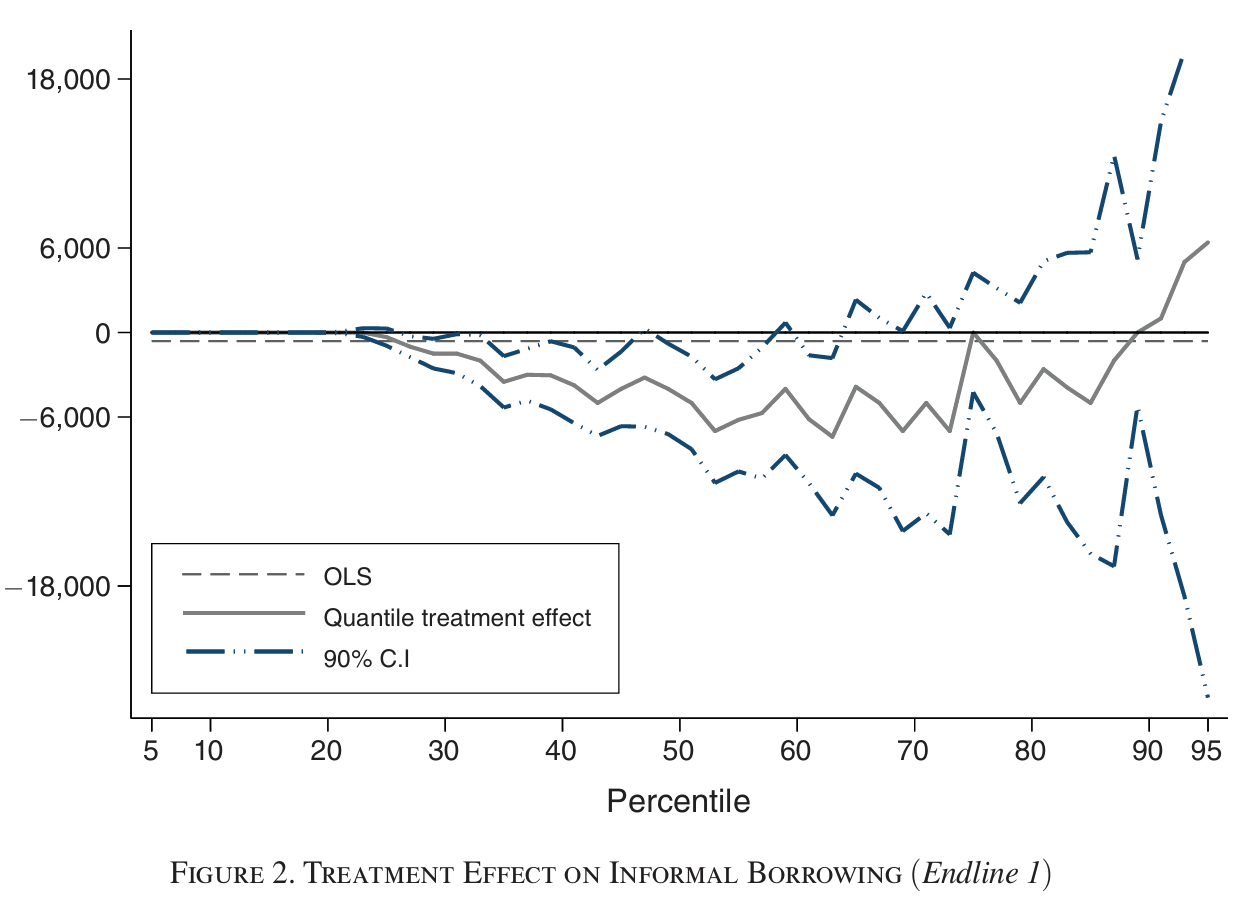
\includegraphics{Images/Banerjee_p38.png}

}

\caption{Estimates of Quantile Treatment Effects from Banerjee \emph{et
al.} (2015, p.~38)}

\end{figure}%

To learn about the quantiles of the treatment effects distribution we
need to employ additional assumptions. In particular, we need to assume
that the treatment preserves the rank of units: perfect rank
correlation. Under this assumption any quantile of the distribution of
treatment effects is equal to the corresponding quantile treatment
effect.

One case where rank is preserved is homogeneous treatment effects.
However, this is somewhat of a redundant case, since homogeneous
treatment effects imply that all quantiles of the treatment effect
distribution are the same and equal to the mean.

\subsection{Randomization in
Economics}\label{randomization-in-economics}

In applied microeconomics, randomized (field) experiments are commonly
referred to as Randomized Control Trials (RCTs). This is a term that has
been borrowed from the medical sciences, where the effectiveness of
drugs and treatments are evaluated using randomized experiments.
Economics RCTs are not necessarily as complex in design as medical
experiments and typically don't include placebo treatments and
double-blind assignment.

While randomization has a long history of use in the laboratory
experiments of Behavioural Economics and Microeconomic Theory research,
its use in applied fields of research - including, Labour, Development,
and Health Economics - is more recent. There are two main barriers to
the use of RCTs in research:

\begin{enumerate}
\def\labelenumi{\arabic{enumi}.}
\item
  They can be very expensive. The time, man-power, and direct cost of
  implementing some RCTs can run into the millions of \$s.
\item
  They can be unethical. Many important research questions cannot be
  studied using a RCT because the decision to treat one group of
  individuals - and therefore exclude another from treatment - is
  unethical.
\end{enumerate}

That does not mean that they are uncommon. Indeed, since the early 2000s
there has been an explosion of research employing RCTs in Economics; in
particular, in the field of Development Economics. In the developed
world, many public policies are now evaluated first using small scale
RCTs before being rolled out to the wider population.

RCTs have come under criticism in Economics. Angus Deaton has been quite
critical of the use of RCTs in Development Economics pointing out
ethical, practical, and conceptual issues with their use. One of his
more substantive critiques relates to the difference bewteen
experimental treatments and real-world policies. RCTs measure the impact
of the assigned treatment, which may differ substantially from a real
world policy. For this reason, RCTs do not always tell us what the
expected impact of a real policy change would be. For further reading on
the topic, see Deaton (2010) and \ldots\ldots{} .

Another critique comes from James Heckman, who argues that internal
validity of RCTs is lost to their lack of \textbf{external validity}. A
randomized experiment can be used to study the (average) treatment
effect of the sampled population, but says nothing about the wider
population, not sampled by the experiment. Given their budgetary
constraints, RCTs are often constrained in terms of the population they
can sample; for example, you may trial a new education policy using a
select sample of 50 schools. The RCT will inform you about the ATE for
that sample of 50 schools, but not necessarily the wider population of
schools. Extrapolation to the wider population requires us to make
additional assumptions that may not be reasonable.

Considering these limitations, there are many important Economics
research questions which may not be appropriate to study using a
randomized experiment. Answering these questions may require us to make
additional assumptions and used more model-based Econometric tools.

Nevertheless, randomization and, in particular, the notion of
unconfounded treatment remains a useful lense through which to evaluate
causal questions in observational settings. For example, we may wish to
study the labour market value of attending a top-ranked university (as
in Krueger) but, for ethical reasons, cannot randomly assign who attends
a top ranked university. In the absence of randomization, it is likely
that selection into treatment (attending a top-ranked university) is
confounded. If randomization is the ``gold standard'', then how distinct
is the observed assignment from random?

\section{Inference under
Randomization}\label{inference-under-randomization}

\subsection{Fisher vs Neyman}\label{fisher-vs-neyman}

When evaluating \textbf{finite samples}, there are two potential null
hypothesis: 1. Fisher's sharp null hypothesis: \[
            \begin{align*}
                &H_0: Y_i(1)=Y_i(0) \quad\forall i=1,...,N \\
                \text{against }&H_1:\;\exists\;i\; \text{s.t.}\;Y_i(1)\neq Y_i(0)
            \end{align*}
            \] 2. Neyman's (finite sample) average treatment effect
(ATE) hypothesis: \[
            \begin{align*}
                &H'_0: \frac{1}{N}\sum_{i=1}^{N}(Y_i(1)-Y_i(0))=0 \\
                \text{against }&H'_1:\frac{1}{N}\sum_{i=1}^{N}(Y_i(1)-Y_i(0))\neq0
        \end{align*}
          \]

\subsection{Fisher's exact p-values}\label{fishers-exact-p-values}

Consider the test statistic, \[
T(W,Y^{obs}) = \bar{Y}^{obs}_t-\bar{Y}^{obs}_c
\]

Since we know the assignment mechanism under randomization, we can
consider other realizations of W, \[
            T(\tilde{W},Y^{obs})
        \] \textbf{under the null hypothesis.}

\par

\begin{itemize}
\tightlist
\item
  \textbf{Why?} Under \(H_0\), \(Y^{obs}=Y(1)=Y(0)\)
\item
  Just need to consider other allocations of \(W\)
\item
  In fact, we can calculate the \textit{exact} distribution of \(T\)
  under the null.
\item
  Can calculate \textit{exact} p-value
\item
  Works for many test-statistics, including rank
\end{itemize}

Suppose we observe the data on outcomes \(Y^{obs}\) and treatment status
\(W\),

\begin{longtable}[]{@{}ll@{}}
\toprule\noalign{}
Y\^{}\{obs\} & W \\
\midrule\noalign{}
\endhead
\bottomrule\noalign{}
\endlastfoot
3 & 1 \\
6 & 0 \\
9 & 1 \\
4 & 1 \\
5 & 0 \\
2 & 0 \\
\end{longtable}

\subsection{Fisher: How does this
work?}\label{fisher-how-does-this-work}

Depending on treatment status, we either observe \(Y_i(0)\) or
\(Y_i(1)\),

\begin{longtable}[]{@{}llll@{}}
\toprule\noalign{}
\(Y^{obs}\) & \(W\) & \(Y(0)\) & \(Y(1)\) \\
\midrule\noalign{}
\endhead
\bottomrule\noalign{}
\endlastfoot
3 & 1 & - & 3 \\
6 & 0 & 6 & - \\
9 & 1 & - & 9 \\
4 & 1 & - & 4 \\
5 & 0 & 5 & - \\
2 & 0 & 2 & \\
\end{longtable}

With this data we can compute any test-static \(T(W,Y^{obs})\). For
example, the standard t-statistic (assuming unequal variances),

\[
T(W,Y^{obs}) = \frac{\hat{\tau}}{\hat{se}(\hat{\tau})} = \frac{\bar{Y}^{obs}_t-\bar{Y}^{obs}_c}{\sqrt{\frac{S^2_c}{N_c}+\frac{S^2_t}{N_t}}}
\] Since the null hypothesis -
\(H_0: Y_i(0)=Y_i(1) \quad\forall\; i=1,...,N\) - \textbf{is sharp}, we
know,

\begin{longtable}[]{@{}llll@{}}
\toprule\noalign{}
\(Y^{obs}\) & \(W\) & \(Y(0)\) & \(Y(1)\) \\
\midrule\noalign{}
\endhead
\bottomrule\noalign{}
\endlastfoot
3 & 1 & {3} & 3 \\
6 & 0 & 6 & {6} \\
9 & 1 & {9} & 9 \\
4 & 1 & {4} & 4 \\
5 & 0 & 5 & {5} \\
2 & 0 & 2 & {2} \\
\end{longtable}

\textbf{under the null}.

We can therefore construct other realizations of the treatment
allocation: \(W'\).

\begin{longtable}[]{@{}
  >{\raggedright\arraybackslash}p{(\columnwidth - 10\tabcolsep) * \real{0.0846}}
  >{\raggedright\arraybackslash}p{(\columnwidth - 10\tabcolsep) * \real{0.0385}}
  >{\raggedright\arraybackslash}p{(\columnwidth - 10\tabcolsep) * \real{0.1923}}
  >{\raggedright\arraybackslash}p{(\columnwidth - 10\tabcolsep) * \real{0.1923}}
  >{\raggedright\arraybackslash}p{(\columnwidth - 10\tabcolsep) * \real{0.2231}}
  >{\raggedright\arraybackslash}p{(\columnwidth - 10\tabcolsep) * \real{0.2692}}@{}}
\toprule\noalign{}
\begin{minipage}[b]{\linewidth}\raggedright
\(Y^{obs}\)
\end{minipage} & \begin{minipage}[b]{\linewidth}\raggedright
\(W\)
\end{minipage} & \begin{minipage}[b]{\linewidth}\raggedright
\(Y(0)\)
\end{minipage} & \begin{minipage}[b]{\linewidth}\raggedright
\(Y(1)\)
\end{minipage} & \begin{minipage}[b]{\linewidth}\raggedright
{\(W'\)}
\end{minipage} & \begin{minipage}[b]{\linewidth}\raggedright
{\(Y^{obs'}\)}
\end{minipage} \\
\midrule\noalign{}
\endhead
\bottomrule\noalign{}
\endlastfoot
3 & 1 & {3} & 3 & {0} & {3} \\
6 & 0 & 6 & {6} & {1} & {6} \\
9 & 1 & {9} & 9 & {1} & {9} \\
4 & 1 & {4} & 4 & {0} & {4} \\
5 & 0 & 5 & {5} & {0} & {5} \\
2 & 0 & 2 & {2} & {1} & {2} \\
\end{longtable}

\[
T(W',Y(1),Y(0)) 
\] Compute for \textbf{all} possible realizations of \(W\), get the
exact distribution of the test static \textbf{under the sharp null
hypothesis}.

\subsection{Neyman's ATE test}\label{neymans-ate-test}

Neyman's null hypothesis is,

\par

\[
H_0:\;\tau^{fs}_{ATE} = 0 \qquad\text{against}\qquad H_0:\;\tau^{fs}_{ATE} \neq 0
\]

We can express,

\[
        \tau^{fs}_{ATE} = \frac{1}{N}\sum_{i=1}^{N}(Y_i(1)-Y_i(0))=\bar{Y}(1)-\bar{Y}(0)
\]

\begin{verbatim}
Then, 
\end{verbatim}

\[
        \hat{\tau} = \bar{Y}^{obs}_t-\bar{Y}^{obs}_c
\]

Is an \textbf{unbiased} estimator for \(\tau^{fs}_{ATE}\).

PROOF {[}ON BOARD{]}

\begin{tcolorbox}[enhanced jigsaw, bottomrule=.15mm, coltitle=black, arc=.35mm, left=2mm, opacityback=0, leftrule=.75mm, colbacktitle=quarto-callout-important-color!10!white, title={Proofs}, toprule=.15mm, bottomtitle=1mm, breakable, colframe=quarto-callout-important-color-frame, opacitybacktitle=0.6, titlerule=0mm, colback=white, rightrule=.15mm, toptitle=1mm]

\[
\begin{aligned}
\hat{\tau} = &\bar{Y}^{obs}_t-\bar{Y}^{obs}_c \\
=&\frac{1}{N_t}\sum_{i:w_i=1}y_i-\frac{1}{N_c}\sum_{i:w_0=1}y_i \\
=&\frac{1}{N_t}\sum_{i=1}w_iy_i-\frac{1}{N_c}\sum_{i=0}(1-w_i)y_i \\
=&\frac{1}{N}[\sum_{i=1}^{N}\frac{w_iy_i}{N_t/N}-\sum_{i=0}^{N}\frac{(1-w_i)y_i}{N_c/N}]
\end{aligned}
\] Neyman Test statisitc -\textgreater{}
\(\mathbf{E}_w[\hat{\tau}|y(1),y(0)]=\tau_{ATE}^{fs}\)

where \(\mathbf[E]_w\) means taking expectation with respect to \(w\)

\[
\begin{aligned}
\mathbf{E}_w[\hat{\tau}|y(1),y(0)] = &\frac{1}{N}[\sum_{i=1}^{N}\frac{\mathbf{E}_w[w_i]y_i}{N_t/N}-\sum_{i=0}^{N}\frac{\mathbf{E}_w[1-w_i]y_i}{N_c/N}] \\
 where &\space \mathbf{E}_w[w_i]=\frac{N_t}{N} \space\space\space\space\space \mathbf{E}_w[1-w_i]=\frac{N_c}{N} \\
=&\frac{1}{N}[\sum_{i=1}^{N}\frac{(N_t/N)y_i}{N_t/N}-\sum_{i=0}^{N}\frac{(N_c/N)y_i}{N_c/N}] \\
=&\frac{1}{N}\sum_{i=1}^{N}(y_i(1)-y_i(0))
\end{aligned}
\]

\end{tcolorbox}

\subsection{Sampling Variance of Neyman
estimator}\label{sampling-variance-of-neyman-estimator}

Remember, with a fixed sample, the source of variation is \(W\).

\begin{itemize}
\tightlist
\item
  \(E_W[W_i]=E_W[W_i^2] = \frac{N_t}{N}\)
\item
  \(Var_W(W_i) = \frac{N_t}{N}\cdot(1-\frac{N_t}{N})\)
\end{itemize}

But we also need to consider the correlation between \(W_i\) and
\(W_{i'}\):

\begin{itemize}
\tightlist
\item
  \(E_W[W_iW_{i'}]=Pr_W(W_i=1)\cdot Pr(W_i=1|W_i=1) = \frac{N_t}{N}\cdot\frac{N_t-1}{N-1}\)
  for \(i\neq i'\)
\end{itemize}

\begin{tcolorbox}[enhanced jigsaw, bottomrule=.15mm, coltitle=black, arc=.35mm, left=2mm, opacityback=0, leftrule=.75mm, colbacktitle=quarto-callout-tip-color!10!white, title={Finite sampling variance of \(\hat{\tau}\)}, toprule=.15mm, bottomtitle=1mm, breakable, colframe=quarto-callout-tip-color-frame, opacitybacktitle=0.6, titlerule=0mm, colback=white, rightrule=.15mm, toptitle=1mm]

\[
                V^{fs}(\hat{\tau}) = \frac{S^2_c}{N_c}+\frac{S^2_t}{N_t}-\frac{S^2_{ct}}{N}
\]

\end{tcolorbox}

\begin{itemize}
\tightlist
\item
  The proof is a little involved!
\end{itemize}

\[
        S^2_c = \frac{1}{N-1}\sum_{i=1}^N (Y_i(0)-\bar{Y}(0))^2
\]

\[
    S^2_t = \frac{1}{N-1}\sum_{i=1}^N (Y_i(1)-\bar{Y}(1))^2
\] **Note, the variance of \(Y(1)\) and \(Y(0)\) need not be the same.
And, \[
        \begin{align*}
        S^2_{ct} &= \frac{1}{N-1}\sum_{i=1}^N (Y_i(1)-Y_i(0)-(\bar{Y}(1)-\bar{Y}(0)))^2 \\
        &=\frac{1}{N-1}\sum_{i=1}^N (Y_i(1)-Y_i(0)-\tau^{fs}_{ATE})^2
        \end{align*}
\]

\begin{itemize}
\item
  Third term captures the sample variation in the unit-level TE.
\item
  If TE are constant (i.e.~\emph{homogenous}), then equals 0.

  We have no way of estimating the \(S^2_{ct}\) since it requires
  observation of both \(Y_i(1)\) and \(Y_i(0)\) for the same unit.
\end{itemize}

\begin{tcolorbox}[enhanced jigsaw, bottomrule=.15mm, coltitle=black, arc=.35mm, left=2mm, opacityback=0, leftrule=.75mm, colbacktitle=quarto-callout-important-color!10!white, title={Theorem: Neyman's variance estimator}, toprule=.15mm, bottomtitle=1mm, breakable, colframe=quarto-callout-important-color-frame, opacitybacktitle=0.6, titlerule=0mm, colback=white, rightrule=.15mm, toptitle=1mm]

If the treatment effect is constant, then an unbiased estimator for the
sampling variance is, \[
        \hat{V}^{neyman} = \frac{s^2_c}{N_c}+\frac{s^2_t}{N_t}
\]

\end{tcolorbox}

where, \[
        s^2_c = \frac{1}{N_c-1}\sum_{i:W_i=0}^N (Y_i^{obs}-\bar{Y}^{obs}_c)^2
\] \[
        s^2_t = \frac{1}{N_t-1}\sum_{i:W_i=1}^N (Y_i^{obs}-\bar{Y}^{obs}_t)^2
\]\\
** Note, this is different to the T-test variance

\subsection{Sampling Variance of Neyman estimator: An
improvement}\label{sampling-variance-of-neyman-estimator-an-improvement}

However, we can improve on this estimator for small samples. If we
assume that \(Y_i(1)-Y_i(0)\) is a constant, then \[
S^2 = S^2_c=S^2_t
\]

\begin{tcolorbox}[enhanced jigsaw, bottomrule=.15mm, coltitle=black, arc=.35mm, left=2mm, opacityback=0, leftrule=.75mm, colbacktitle=quarto-callout-important-color!10!white, title={Constant variance estimator}, toprule=.15mm, bottomtitle=1mm, breakable, colframe=quarto-callout-important-color-frame, opacitybacktitle=0.6, titlerule=0mm, colback=white, rightrule=.15mm, toptitle=1mm]

If the treatment effect is constant, then a more precise, unbiased
estimator for the sampling variance is, \[
            \hat{V}^{const} = s^2\cdot\left(\frac{1}{N_c}+\frac{1}{N_t}\right)
\]

\end{tcolorbox}

\begin{verbatim}
where, 
\end{verbatim}

\[
        s^2 = \frac{1}{N-2}\cdot\left(s^2_c\cdot(N_c-1)+s^2_t\cdot(N_t-1)\right)
\] ** These equations should be fairly familiar.

\subsection{Neyman hypothesis test}\label{neyman-hypothesis-test}

To conduct inference we need to know the distribution of the
test-statistic, not just the variance.

Potential approaches:

\begin{enumerate}
\def\labelenumi{\arabic{enumi}.}
\tightlist
\item
  Use a normal approximation of the randomization distribution of
  \(\hat{\tau}\)
\item
  Approximate distribution of \(\hat{V}\) by chi-squared and use
  t-distribution. \[
        t = \frac{\hat{\tau}}{\sqrt{\hat{V}}}
  \]
\end{enumerate}

Confidence intervals, \[
    CI^{0.95}(\tau^{fs}_{ATE}) \approxeq \left[\hat{\tau}+z_{0.025}\cdot\sqrt{\hat{V}},\hat{\tau}+z_{0.975}\cdot\sqrt{\hat{V}}\right]
\]\\
or \[
        CI^{0.95}(\tau^{fs}_{ATE}) \approxeq \left[\hat{\tau}+t_{N-2,0.025}\cdot\sqrt{\hat{V}},\hat{\tau}+t_{N-2,0.975}\cdot\sqrt{\hat{V}}\right]
\]

\subsection{Fisher vs Neyman}\label{fisher-vs-neyman-1}

Remember the differences in the null hypotheses:

\par

\begin{itemize}
\tightlist
\item
  Fisher {[}\textbf{exact}{]}:
  \(H_0: Y_i(1)=Y_i(0) \quad\forall i=1,...,N\)
\item
  Neyman: \(H'_0: \frac{1}{N}\sum_{i=1}^{N}(Y_i(1)-Y_i(0))=0\)
\end{itemize}

From Imbens and Wooldridge (2009, p.23)\footnote{This is the notation
  used Imbens and Rubin (2015). I have not introduced it in class to
  avoid having too much notation; however, it is helpful here.},

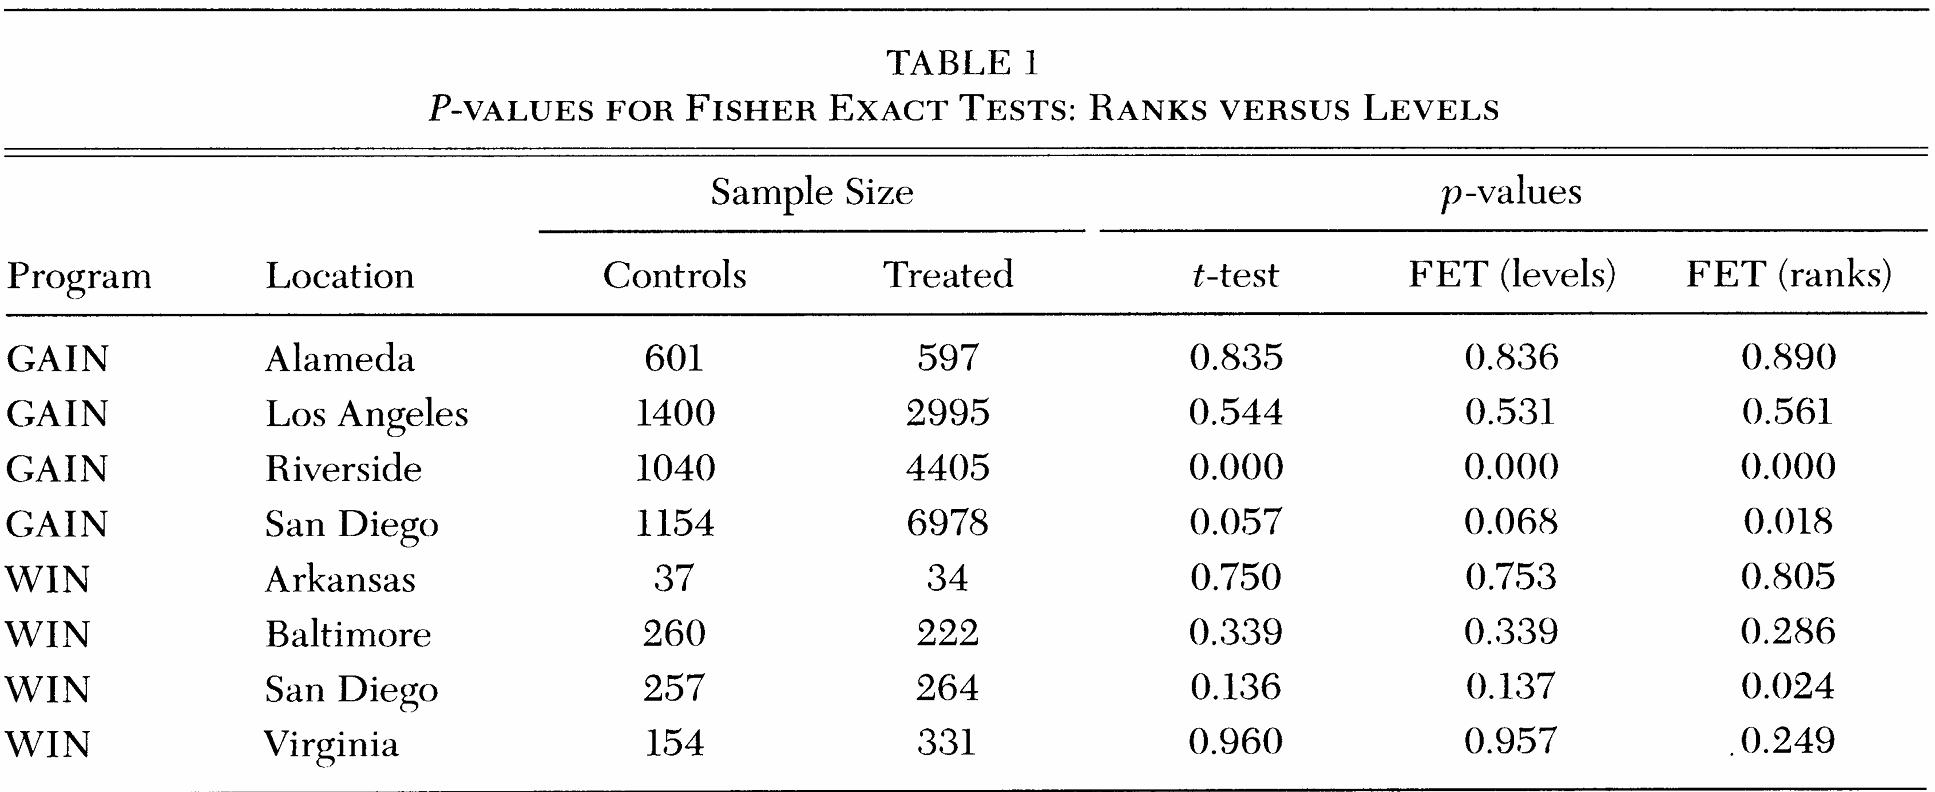
\includegraphics{Images/table1_imbenswooldridge2009.png}

\subsection{Neyman: Super-population
equivalent}\label{neyman-super-population-equivalent}

Suppose we think of the sample N as a \textbf{random} draw from a
potentially infinite super-population,

\begin{tcolorbox}[enhanced jigsaw, bottomrule=.15mm, coltitle=black, arc=.35mm, left=2mm, opacityback=0, leftrule=.75mm, colbacktitle=quarto-callout-important-color!10!white, title={Result}, toprule=.15mm, bottomtitle=1mm, breakable, colframe=quarto-callout-important-color-frame, opacitybacktitle=0.6, titlerule=0mm, colback=white, rightrule=.15mm, toptitle=1mm]

\[
                E[\hat{\tau}] = E[\tau^{fs}_{ATE}] = \tau_{ATE}
\] \[
                V(\hat{\tau}) = E\left[(\bar{Y}^{obs}_t-\bar{Y}^{obs}_c-E[\bar{Y}^{obs}_t-\bar{Y}^{obs}_c])^2\right]= \frac{\sigma^2_c}{N_c}+\frac{\sigma^2_t}{N_t}
\] Proof will be provided on Moodle.

\end{tcolorbox}

\begin{itemize}
\tightlist
\item
  \(\hat{V}^{neyman}\) is an unbiased estimator for \(V\), \textbf{even
  with heterogeneous TE's}.
\item
  \(\hat{V}^{neyman}\) is a better default choice.
\end{itemize}

VARIANCE PROOF ON MOODLE

\section{Balance tests}\label{balance-tests}

\subsection{Testing for balance in
covariates}\label{testing-for-balance-in-covariates}

All Randomized Control Trials should provide some variant of a balance
table: a table comparing the means of pre-treatment covariates in each
of the treatment groups.

For example, (Oreopoulus, 2011, p.158)\footnote{Oreopoulos, P. 2011,
  ``Why Do Skilled Immigrants Struggle in the Labor Market? A Field
  Experiment with Thirteen Thousand Resumes'', American economic
  journal. Economic policy, vol.~3, no. 4, pp. 148-171.}

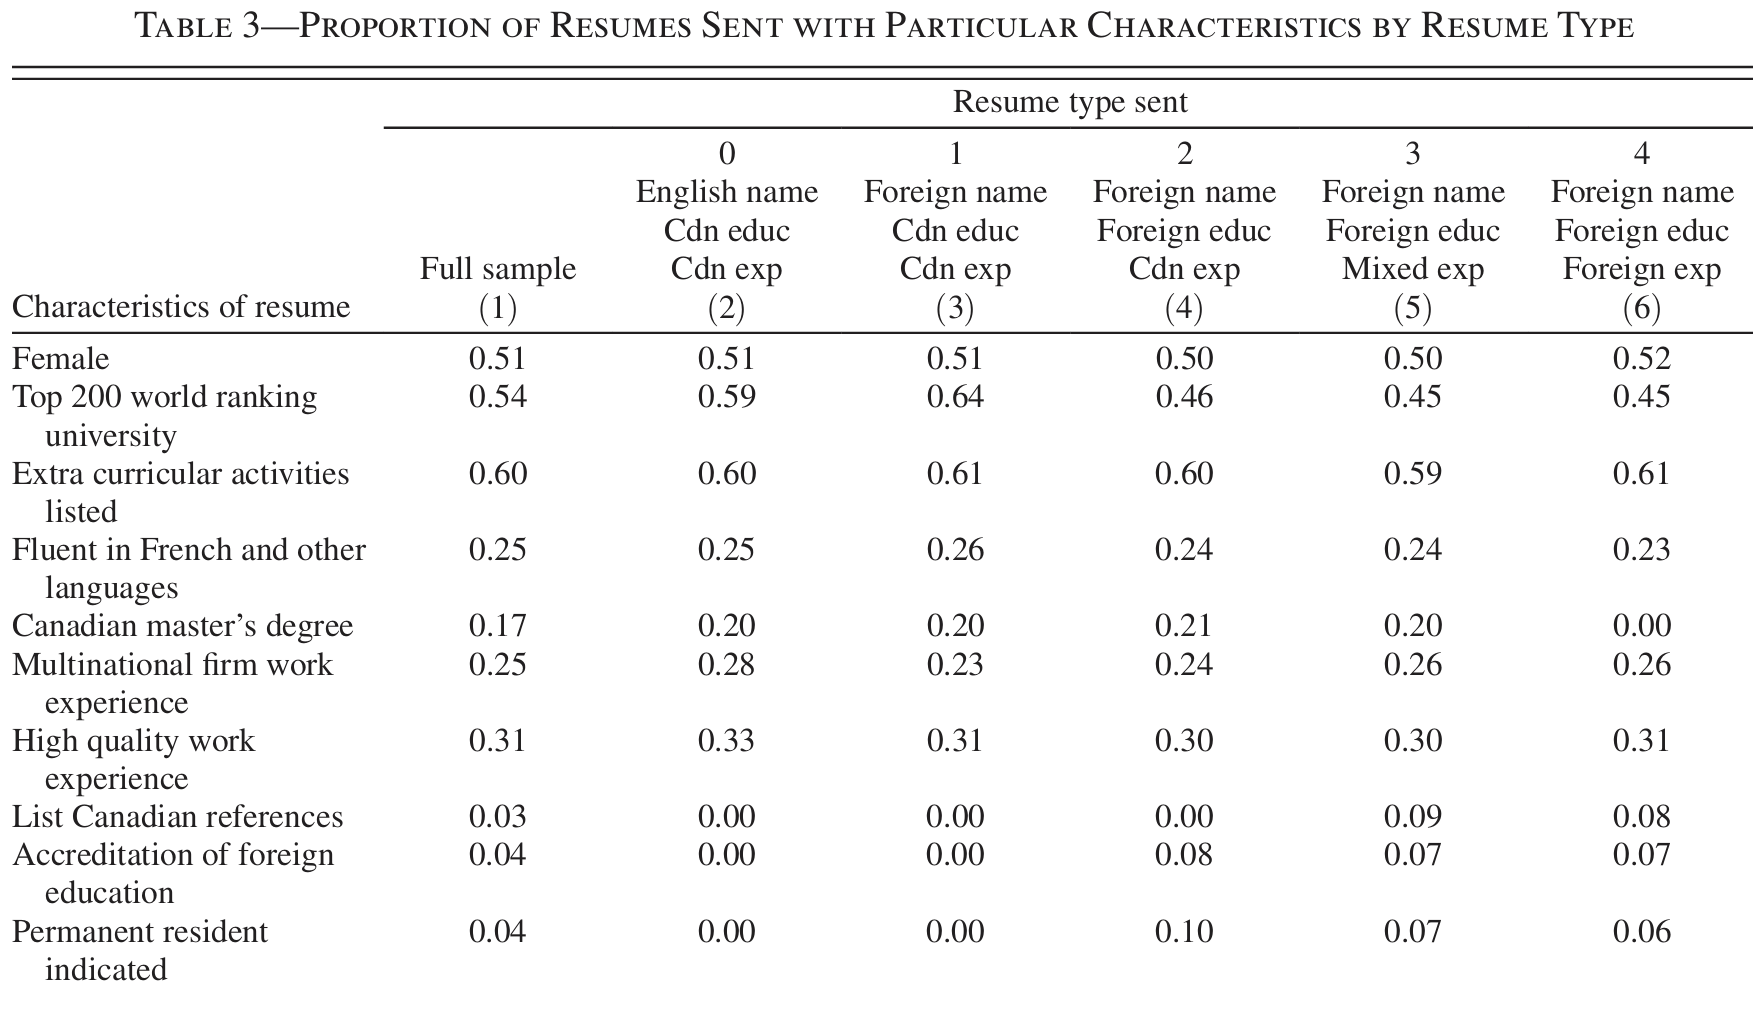
\includegraphics{Images/Oreopoulus_Balance_1.png}

These tests are typically based on the ANOVA ({AN}alysis {O}f
{VA}riance) test.\footnote{Common Alternatives include Multivariate
  ANOVA (MANOVA) and Analysis of Covariance (ANCOVA)}

\begin{itemize}
\tightlist
\item
  Decomposes TSS into,\footnote{Check your EC124 notes on this.}
\end{itemize}

\[
                TSS = \sum_{k=1}^{K}\sum_{i=1}^{N(k)}(X_{ik}-\bar{X})^2 = \underbrace{\sum_{k=1}^{K}\sum_{i=1}^{N(k)}(X_{ik}-\bar{X}_k)^2}_\text{residual/within}+\underbrace{\sum_{k=1}^{K}N(k)(\bar{X}_k-\bar{X})^2}_\text{explained/between}
\]

\begin{itemize}
\tightlist
\item
  The F-statistic, \[
              F-stat =\frac{ESS/(K-1)}{RSS/(N-K)} = \frac{\text{explained/between variance}}{\text{residual/within variance}}
  \]
\end{itemize}

This is to estimating the linear regression model,

\[
            X_i = \beta_0 + \beta_1D_{i1}+...+ \beta_KD_{i,K-1}+\varepsilon_i
\]

where the dummy variables indicate \(K-1\) groups. Test the joint linear
hypothesis, \[
            H_0: \beta_1 = ... = \beta_{K-1} = 0
\]

against, \[
            H_1: \text{at least one }\beta_j\neq0\qquad j=1,...,K-1
\]

\begin{itemize}
\tightlist
\item
  Note, you should be wary of testing each \(\beta\) coefficient
  separately. \textbf{Why?}
\end{itemize}

For example, Dupas and Robinson (2013, p.1150)\footnote{Dupas, P. \&
  Robinson, J. 2013, ``Why Don't the Poor Save More? Evidence from
  Health Savings Experiments'', The American economic review, vol.~103,
  no. 4, pp.~1138-1171.}

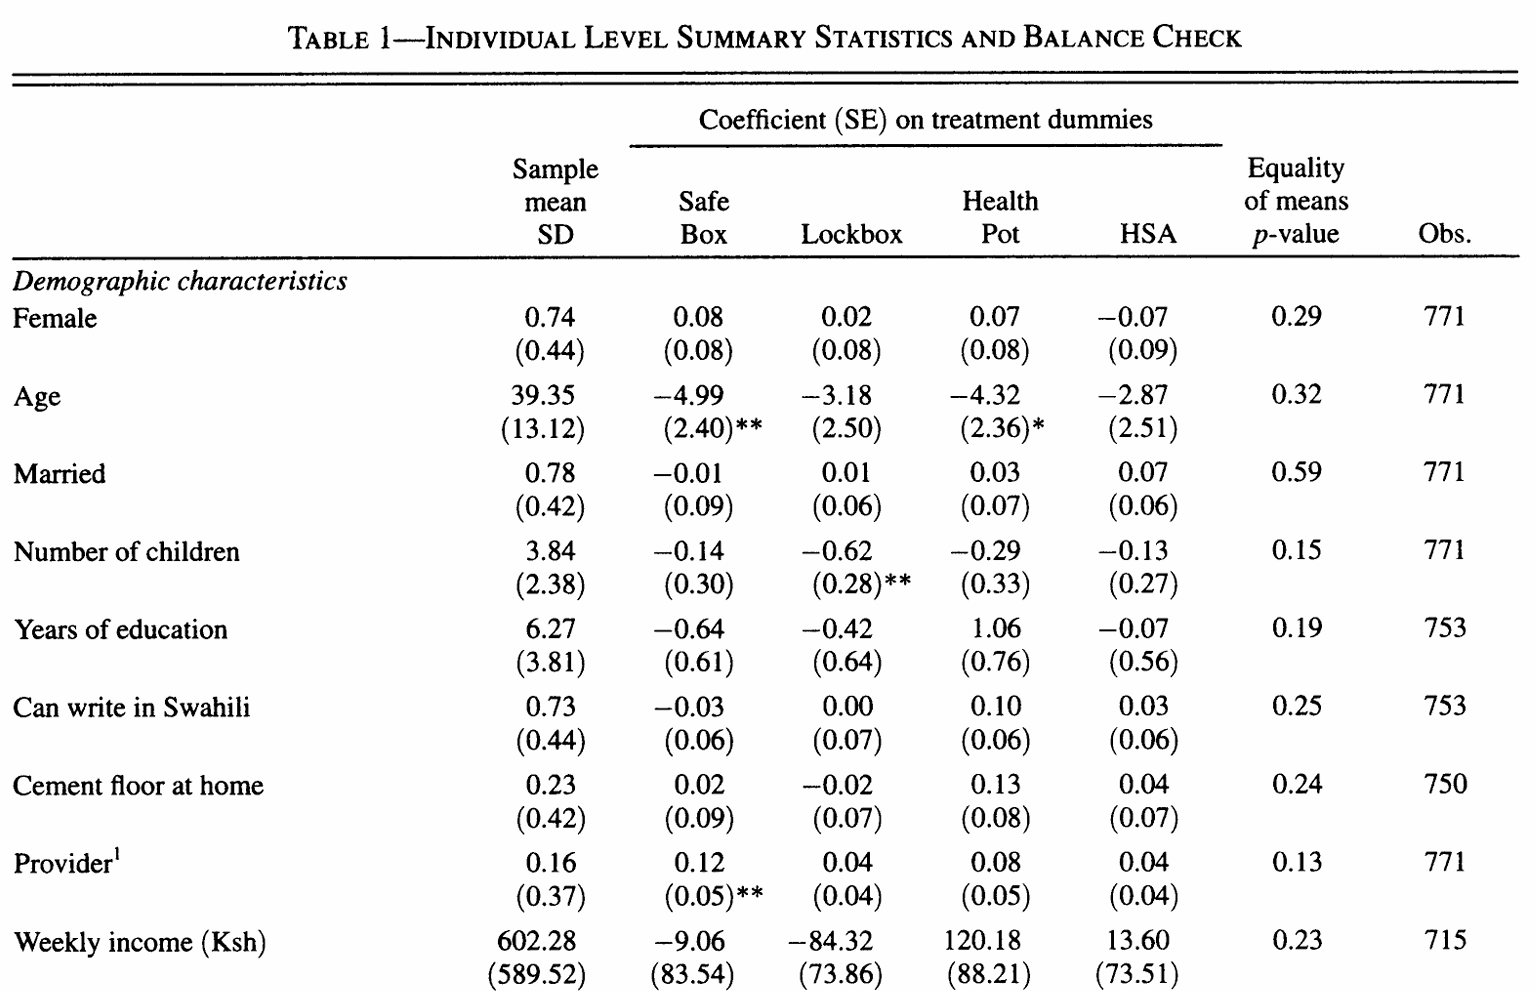
\includegraphics{Images/Dupas_Baseline_1.png}

It is important to remember,

\par

\begin{itemize}
\tightlist
\item
  Balance tests provide support for unconfoundedness (i.e. randomization
  has worked)
\item
  We can test for differences in observables.
\item
  We cannot rule out selection on unobservables.
\item
  Partially rely on sufficiently large sample size.
\end{itemize}

\subsection{Next-up}\label{next-up}

\begin{itemize}
\tightlist
\item
  Evaluating RCT's with Linear Regression and (one of) Angus Deaton's
  critiques
\item
  Covariates, Efficiency, and Power\\
\item
  Good and Bad Controls
\item
  Intent to Treat and some examples
\end{itemize}

\section{Evaluating RCTs using a Linear Regression
Model}\label{evaluating-rcts-using-a-linear-regression-model}

\subsection{Linear Regression Model}\label{linear-regression-model}

Consider the linear regression \emph{model}, \[
            Y_i = \alpha+\beta W_i + \varepsilon_i
\] where, intuitively, \(Y_i = Y^{obs}_i\). The OLS estimator for the
vector of parameters \((\alpha,\beta)\) is defined as, \[
            (\hat{\alpha}^{OLS},\hat{\beta}^{OLS}) = \underset{a,b}{argmin} \sum_{i=1}^{N}(Y_i-a-b W_i)^2
\] We know that in the case of a simple linear regression model, \[
            \hat{\beta}^{OLS} = \frac{\sum_{i=1}^{N}(W_i-\bar{W})(Y_i-\bar{Y})}{\sum_{i=1}^{N}(W_i-\bar{W})^2} = (W'M_\ell W)^{-1}W'M_\ell Y
\]

the sample analogue of \(\beta = \frac{Cov(W_i,Y_i)}{Var(W_i)}\).

Since \(\bar{W}=\frac{N_t}{N}\), we can show that \footnote{Do ensure
  that you can show this.}

\[
            \hat{\beta}^{OLS} = \bar{Y}^{obs}_t-\bar{Y}^{obs}_c = \hat{\tau}
\]

Which we know is an unbiased estimator for both \(\tau_{ATE}^{fs}\) and
\(\tau_{ATE}\).

\par

\begin{itemize}
\tightlist
\item
  \(\hat{\beta}^{OLS}\) is an unbiased estimate of the (average) causal
  effect, assuming unconfoundedness (i.e.~completely random experiment).
\end{itemize}

We want to create a mapping from potential outcomes to a linear
regression model. Recall, \[
            Y^{obs}_i = Y_i(0)+W_i(Y_i(1)-Y_(0))
\] Let's define\footnote{Here I am avoiding finite sample notation. This
  is not a big issue as you can always define the expectation as an
  average in the finite sample.},

\[
        \begin{align*}
            \mu &=E[Y_i(0)] \\
            \tau_{ATE} &= E[Y_i(1)-Y_i(0)]
        \end{align*}
\]\\
We want to show that we can express \(Y^{obs}_i\) as a linear regression
model, \[
            Y^{obs}_i=\mu+\tau_{ATE}W_i+\varepsilon_i
\]

\subsection{Endogeneity}\label{endogeneity}

We write the error term from the linear regression model as function of
these parameters and the potential outcomes in the following way, \[
        \begin{align*}
            \varepsilon_i   &=Y_i(0)- \mu+W_i\cdot(Y_i(1)-Y_i(0)-\tau_{ATE}) \\
                            &=\begin{cases*}
                                Y^{obs}_i-\mu \qquad\qquad\quad \text{if}\quad W_i=0 \\
                                Y^{obs}_i-\mu-\tau_{ATE} \qquad \text{if}\quad W_i=1
                            \end{cases*} \\
                            &=\begin{cases*}
                                Y_i(0)-E[Y_i(0)] \qquad\qquad\qquad\qquad\qquad\qquad\qquad\qquad\quad \text{if}\quad W_i=0 \\
                                Y_i(0)-E[Y_i(0)]+\underbrace{\left(Y_i(1)-Y_i(0)-E[Y_i(1)-Y_i(0)]\right)}_\text{heterogeneity} \quad \text{if}\quad W_i=1
                            \end{cases*}                        
        \end{align*}
\] Note, for a more straight forward mapping we can assume homogenous
TEs, \[
            (Y_i(1)-Y_i(0)) = \tau\qquad \forall i
\]

\[
\begin{align}
            Y_i &= Y_i(0)+W_i\cdot\underbrace{(Y_i(1)-Y_i(0))}_{\tau} \\
                &=E[Y_i(0)]+\tau W_i+\underbrace{Y_i(0)-E[Y_i(0)]}_{\varepsilon_i} \\
                &=\mu+\tau W_i + \varepsilon_i
\end{align}
\] As an assignment mechanism, randomization gives us unconfoundedness,
\[
            (Y_i(1),Y_i(0))\perp W_i
\] So, then we can consider the conditional expectations of
\(\varepsilon_i\),

\par

\begin{itemize}
\tightlist
\item
  \(W_i=0\) \[
          \begin{align*}
              E[\varepsilon_i|W_i=0] &= E[Y_i(0)- \mu + W_i\cdot(Y_i(1)-Y_i(0)-\tau_{ATE})|W_i=0] \\
              &= E[Y_i(0)- \mu|W_i=0] \\
              &=E[Y_i(0)|W_i=0]-E[Y_i(0)] = 0
          \end{align*}
  \]
\item
  \(W_i=1\) \[
          \begin{align*}
              E[\varepsilon_i|W_i=1] &= E[Y_i(0)- \mu + W_i\cdot(Y_i(1)-Y_i(0)-\tau_{ATE})|W_i=1] \\
              &= E[Y_i(1)-\tau_{ATE} - \mu|W_i=1] \\
              &=E[Y_i(1)|W_i=1]-E[Y_i(0)]-E[Y_i(1)-Y_i(0)] = 0
          \end{align*}
  \] Unconfoundedness gives you mean independence.
\end{itemize}

\subsection{Inference}\label{inference}

Suppose we assume homoskedasticity: \(\sigma_i^2=\sigma^2\)\\
\[
        \begin{align*}
            \hat{\sigma}^2 = \frac{1}{N-2}\sum_{i=1}^N \hat{\varepsilon}_i^2&= \frac{1}{N-2}\sum_{i=1}^N  (Y_i-\hat{\alpha}^{OLS}-\hat{\beta}^{OLS}W_i)^2 \\
            &=\frac{1}{N-2}\sum_{i=1}^N  \left(Y_i-\bar{Y}-(\bar{Y}^{obs}_t-\bar{Y}^{obs}_c)\cdot(W_i-\bar{W})\right)^2 \\
            &=\frac{1}{N-2}\left(\sum_{i:W_i=0}^N(Y_i-\bar{Y}^{obs}_c)^2+\sum_{i:W_i=1}^N(Y_i-\bar{Y}^{obs}_t)^2\right) \\
            &=s^2
        \end{align*}
\]

where, \[
        s^2 = \frac{1}{N-2}\cdot\left(s^2_c\cdot(N_c-1)+s^2_t\cdot(N_t-1)\right)
\] ** Check to see if you can show this.

\subsection{Deaton's critique}\label{deatons-critique}

Angus Deaton has made a number of criticisms against the use of RCTs in
(Development) Economics. One of these is the misuse of linear
regression:\footnote{Deaton, A. 2010, ``Instruments, Randomization, and
  Learning about Development'', Journal of economic literature, vol.~48,
  no. 2, pp. 424-455.}

\begin{tcolorbox}[enhanced jigsaw, bottomrule=.15mm, coltitle=black, arc=.35mm, left=2mm, opacityback=0, leftrule=.75mm, colbacktitle=quarto-callout-tip-color!10!white, title={Deaton (2010, p.442)}, toprule=.15mm, bottomtitle=1mm, breakable, colframe=quarto-callout-tip-color-frame, opacitybacktitle=0.6, titlerule=0mm, colback=white, rightrule=.15mm, toptitle=1mm]

``However, the standard error of \(\beta_1\) from the OLS regression is
not generally correct. One problem is that the variance among the
experimentals may be different from the variance among the controls, and
to assume that the experiment \textit{does not} affect the variance is
very much against the minimalist spirit of RCTs.''

\end{tcolorbox}

The standard OLS variance estimator for \(\hat{\beta}^{OLS}\) is, \[
        \hat{V}^{homosk} = \frac{\hat{\sigma}^2}{\sum_{i=1}^{N}(W_i-\bar{W})^2}=s^2\cdot\left(\frac{1}{N_c}+\frac{1}{N_t}\right)=\hat{V}^{const}
\] If instead you estimate heteroskedastic standard
errors,\footnote{Some texts scale the heteroskedasticity-robust variance estimator by $N/(N-2)$ (e.g., Stock and Watson, 2020, p.180). With or without the rescaling, you can show that this equality is not exact, given the formulae for $s^2_c$ and $s^2_t$ from lecture 2.1. In this case, you can show that $\hat{V}^{hetero}= \frac{\tilde{s}^2_c}{N_c}+\frac{\tilde{s}^2_t}{N_t}$, where $\tilde{s}^2_c$ and $\tilde{s}^2_t$ are scaled by $N_c$ and $N_t$, respectively. Not by $N_c-1$ and $N_t-1$.}
\[
            \hat{V}^{hetero} = \frac{\sum_{i=1}^{N}\hat{\varepsilon}_i^2\cdot(W_i-\bar{W})^2}{\left(\sum_{i=1}^{N}(W_i-\bar{W})^2\right)^2} \approxeq \frac{s^2_c}{N_c}+\frac{s^2_t}{N_t}=\hat{V}^{neyman}
\]

\begin{tcolorbox}[enhanced jigsaw, bottomrule=.15mm, coltitle=black, arc=.35mm, left=2mm, opacityback=0, leftrule=.75mm, colbacktitle=quarto-callout-tip-color!10!white, title={Deaton (2010, p.442)}, toprule=.15mm, bottomtitle=1mm, breakable, colframe=quarto-callout-tip-color-frame, opacitybacktitle=0.6, titlerule=0mm, colback=white, rightrule=.15mm, toptitle=1mm]

``If the regression \ldots{} is run with the standard heteroskedasticity
correction to the standard error, the result will be the same as the
formula for the standard error of the difference between two means, but
not otherwise except in the special case where there are equal numbers
of experimental and controls, in which case it turns out that the
correction makes no difference and the OLS standard error is correct. It
is not clear in the experimental development literature whether the
correction is routinely done in practice\ldots{}''

\end{tcolorbox}

\section{Adding covariates}\label{adding-covariates}

\subsection{Adding covariates}\label{adding-covariates-1}

Let us consider the linear regression model, \[
            Y_i = \alpha+\beta W_i + X_i'\gamma+\epsilon_i
\]

where,

\par

\begin{itemize}
\tightlist
\item
  \(W_i\) is assigned according to a completely random experiment
\item
  \(X_i\) is a \(k\times 1\) vector of \textbf{pre-treatment} covariates
\item
  the linear function \textbf{need not} be correctly specified
\end{itemize}

Note: we are not interested in the interpretation of the \(\gamma\)'s or
\(\alpha\).

\begin{tcolorbox}[enhanced jigsaw, bottomrule=.15mm, coltitle=black, arc=.35mm, left=2mm, opacityback=0, leftrule=.75mm, colbacktitle=quarto-callout-important-color!10!white, title={Theorem (Imbens and Rubin, 2015, p.123)}, toprule=.15mm, bottomtitle=1mm, breakable, colframe=quarto-callout-important-color-frame, opacitybacktitle=0.6, titlerule=0mm, colback=white, rightrule=.15mm, toptitle=1mm]

Suppose we conduct a \textbf{completely randomized experiment} in a
sample drawn at random from an infinite population. Then,

\par

\begin{enumerate}
\def\labelenumi{\arabic{enumi}.}
\tightlist
\item
  \(plim\;\hat{\beta}=\tau_{ATE}\)
\item
  The asymptotic distribution of \(\hat{\beta}\) is normal.
\end{enumerate}

\end{tcolorbox}

This is a powerful result!

\par

\begin{itemize}
\tightlist
\item
  We are agnostic about the Conditional Expectation Function:
  \(E[Y_i|W_i,X_i']\).
\item
  And the model need not be correctly specified.
\end{itemize}

\subsection{Small sample bias}\label{small-sample-bias}

Unfortunately, in small samples \(\hat{\beta}^{OLS}\) is a biased
estimator of \(\tau_{ATE}\).\footnote{Focus on the intuition of the
  results, not the equation. Taken from Deaton's (2010, p.444)
  discussion of Freedman (2008). In this equation \(X_i\) is single
  covariate.}

\begin{itemize}
\tightlist
\item
  The bias is \(\psi/N\) and \(\psi\) is given by, \[
              \psi = -\lim \frac{1}{N}\sum_{i=1}^N (\tau_i-\tau_{ATE})f(X_i)
  \]
\item
  The source of the bias lies in the correlation between the unit-level
  treatment effect and the covariates.
\item
  Recall, treatment is independent of the covariates.
\item
  But, the individual level treatment effect may not be.
\end{itemize}

\begin{tcolorbox}[enhanced jigsaw, bottomrule=.15mm, coltitle=black, arc=.35mm, left=2mm, opacityback=0, leftrule=.75mm, colbacktitle=quarto-callout-tip-color!10!white, title={In practice}, toprule=.15mm, bottomtitle=1mm, breakable, colframe=quarto-callout-tip-color-frame, opacitybacktitle=0.6, titlerule=0mm, colback=white, rightrule=.15mm, toptitle=1mm]

Include covariates and be wary if the estimated coefficient changes
substantially.

\end{tcolorbox}

\subsection{Efficiency gains}\label{efficiency-gains}

With covariates, the sampling variance of the OLS estimator is reduced.
Here are the estimators:\footnote{Subject of first seminar.}

\[
\hat{V}^{hetero} = \frac{1}{N(N-k)}\cdot\frac{\sum_{i=1}^{N}(W_i-\bar{W})^2(Y_i-\hat{\alpha}^{OLS}-\hat{\beta}^{OLS}-X_i'\hat{\gamma}^{OLS})^2}{\left(\bar{W}(1-\bar{W})\right)^2}
\] or \[
            \hat{V}^{homosk} = \frac{1}{N(N-k)}\cdot\frac{\sum_{i=1}^{N}(Y_i-\hat{\alpha}^{OLS}-\hat{\beta}^{OLS}-X_i'\hat{\gamma}^{OLS})^2}{\bar{W}(1-\bar{W})}
\] where \(k\) is the number of parameters estimated (including the
constant).

\par

\begin{itemize}
\tightlist
\item
  Note, this holds only for \textbf{good covariates}
\end{itemize}

\subsection{Good controls}\label{good-controls}

The question of good and bad controls is \textbf{very}
important.\footnote{Here I am being more general over the choice of the
  estimator \(\hat{\tau}\) and I am approximating the distribution of
  the test-statistic with the standard normal.}

\begin{tcolorbox}[enhanced jigsaw, bottomrule=.15mm, coltitle=black, arc=.35mm, left=2mm, opacityback=0, leftrule=.75mm, colbacktitle=quarto-callout-note-color!10!white, title={Good control}, toprule=.15mm, bottomtitle=1mm, breakable, colframe=quarto-callout-note-color-frame, opacitybacktitle=0.6, titlerule=0mm, colback=white, rightrule=.15mm, toptitle=1mm]

A covariate that is not an outcome of the experiment.

\end{tcolorbox}

\begin{itemize}
\tightlist
\item
  Variables measured at baseline,
\item
  or individual characteristics that cannot change with the experiment
  (e.g.~age).
\end{itemize}

What about stratification?

\par

\begin{itemize}
\tightlist
\item
  You should include stratifying variables in the model
\item
  Stratification improves precision.
\end{itemize}

\subsection{Minimizing Variance}\label{minimizing-variance}

Note, in the variance formulae we have the term in the denominator, \[
            \sum_{i=1}^N(W_i-\bar{W})^2 = N\bar{W}(1-\bar{W})
\]

\begin{verbatim}
    TRY TO SHOW THIS
\end{verbatim}

Which comes from the sample variance of the treatment variable.

\par

To reduce the variance, we can maximize this function. This yields the
solution,

\[
        \bar{W}^*=0.5
\]

\begin{itemize}
\tightlist
\item
  \textbf{Equal assignment is efficient.}
\end{itemize}

\subsection{Under-powered}\label{under-powered}

RCTs often face the risk that they are \textbf{under-powered}. :::
\{.allout-note icon=``false''\} \#\# Power The probability of rejecting
the null hypothesis (\(H_0: \tau=0\); i.e., of no effect) when it is
\textbf{false}. \[
                \theta(\tau_0)=Pr(\text{Reject }H_0|\tau=\tau_0)
\] :::

Recall, that we reject \(H_0: \tau=0\) when \footnote{Here I am being
  more general over the choice of the estimator \(\hat{\tau}\) and I am
  approximating the distribution of the test-statistic with the standard
  normal.}

\[
            |S|>z_{1-\alpha/2}\Longleftrightarrow |\hat{\tau}/se(\hat{\tau})|>z_{1-\alpha/2}
\] Where \(S\) is the test-statistic.

\[
        \begin{align*}
            \theta(\tau_0)=&Pr(|\hat{\tau}/se(\hat{\tau})|>z_{1-\alpha/2}|\tau=\tau_0) \\
            =&Pr(\hat{\tau}/se(\hat{\tau})<z_{\alpha/2}|\tau=\tau_0)+Pr(\hat{\tau}/se(\hat{\tau})>z_{1-\alpha/2}|\tau=\tau_0) \\
            =&Pr\left(\frac{\hat{\tau}-\tau_0}{se(\hat{\tau})}<z_{\alpha/2}-\frac{\tau_0}{se(\hat{\tau})}|\tau=\tau_0\right)\\
            &+Pr\left(\frac{\hat{\tau}-\tau_0}{se(\hat{\tau})}>z_{1-\alpha/2}-\frac{\tau_0}{se(\hat{\tau})}|\tau=\tau_0\right) \\
            =&Pr\left(Z<z_{\alpha/2}-\frac{\tau_0}{se(\hat{\tau})}|\tau=\tau_0\right)+Pr\left(Z>z_{1-\alpha/2}-\frac{\tau_0}{se(\hat{\tau})}|\tau=\tau_0\right)
        \end{align*}
\]\\
Given the shape of the normal distribution, \(\theta(\tau_0)\) is
increasing in \(\tau_0/se(\hat{\tau})\):

\par

\begin{itemize}
\tightlist
\item
  Power is increasing in the absolute value of \(\tau_0\)
\item
  Power decreasing in the \(Var(\hat{\tau})\Rightarrow\) power is
  \textbf{increasing in N}.
\end{itemize}

\section{The Microfinance `Miracle': A Case of
ITT}\label{the-microfinance-miracle-a-case-of-itt}

\subsection{The Microfinance `Miracle'}\label{the-microfinance-miracle}

`{The Miracle of Microfinance? Evidence from a Randomized
Evaluation}\footnote{{Banerjee, A., Duflo, E., Glennerster, R. \&
  Kinnan, C. 2015, ``The Miracle of Microfinance? Evidence from a
  Randomized Evaluation'', American economic journal. Applied economics,
  vol.~7, no. 1, pp. 22-53.}}'

\par

\begin{itemize}
\tightlist
\item
  Microfinance was seen as a `silver bullet' for fighting poverty, but
  robust evidence was scarce.
\item
  Existing evidence based on self-selected clients - not causal.
\item
  {Setting:} Hyderabad, India, capital of Andrha Pradesh
\item
  {Sample:} randomly treat 52 (out of 104) neighbourhoods with new
  Spandana branch.
\item
  {Data Collection:} survey households 18 months, and then 42 months
  after treatment (N=6,850).
\item
  {Research Design:} ``focus here on reduced-form/intent-to-treat
  estimates'\,' because of spillover or general equilibrium effects.
\end{itemize}

\emph{``given the sampling frame, ours will be an intent-to-treat (ITT)
analysis on a sample of''likely borrowers.'' This is thus neither the
effect on those who borrow nor the average effect on the neighborhood.
Rather, it is the average effect of easier access to microfinance on
those who are its primary targets.'\,' (p.35)}

\textbf{Intention-To-Treat (ITT)}

\par

\begin{itemize}
\tightlist
\item
  Based on initial random assignment (i.e.~reduced form)
\item
  Not on take-up or receipt of treatment
\end{itemize}

\emph{``The main drawback of these ITT analyses is that they do not
answer questions about causal effects of the receipt of treatment
itself, only about causal effects of the assignment to treatment.''
(Imbens and Rubin, 2015, p.515)}\footnote{\emph{More generally used in
  discussion of non-compliance.}}

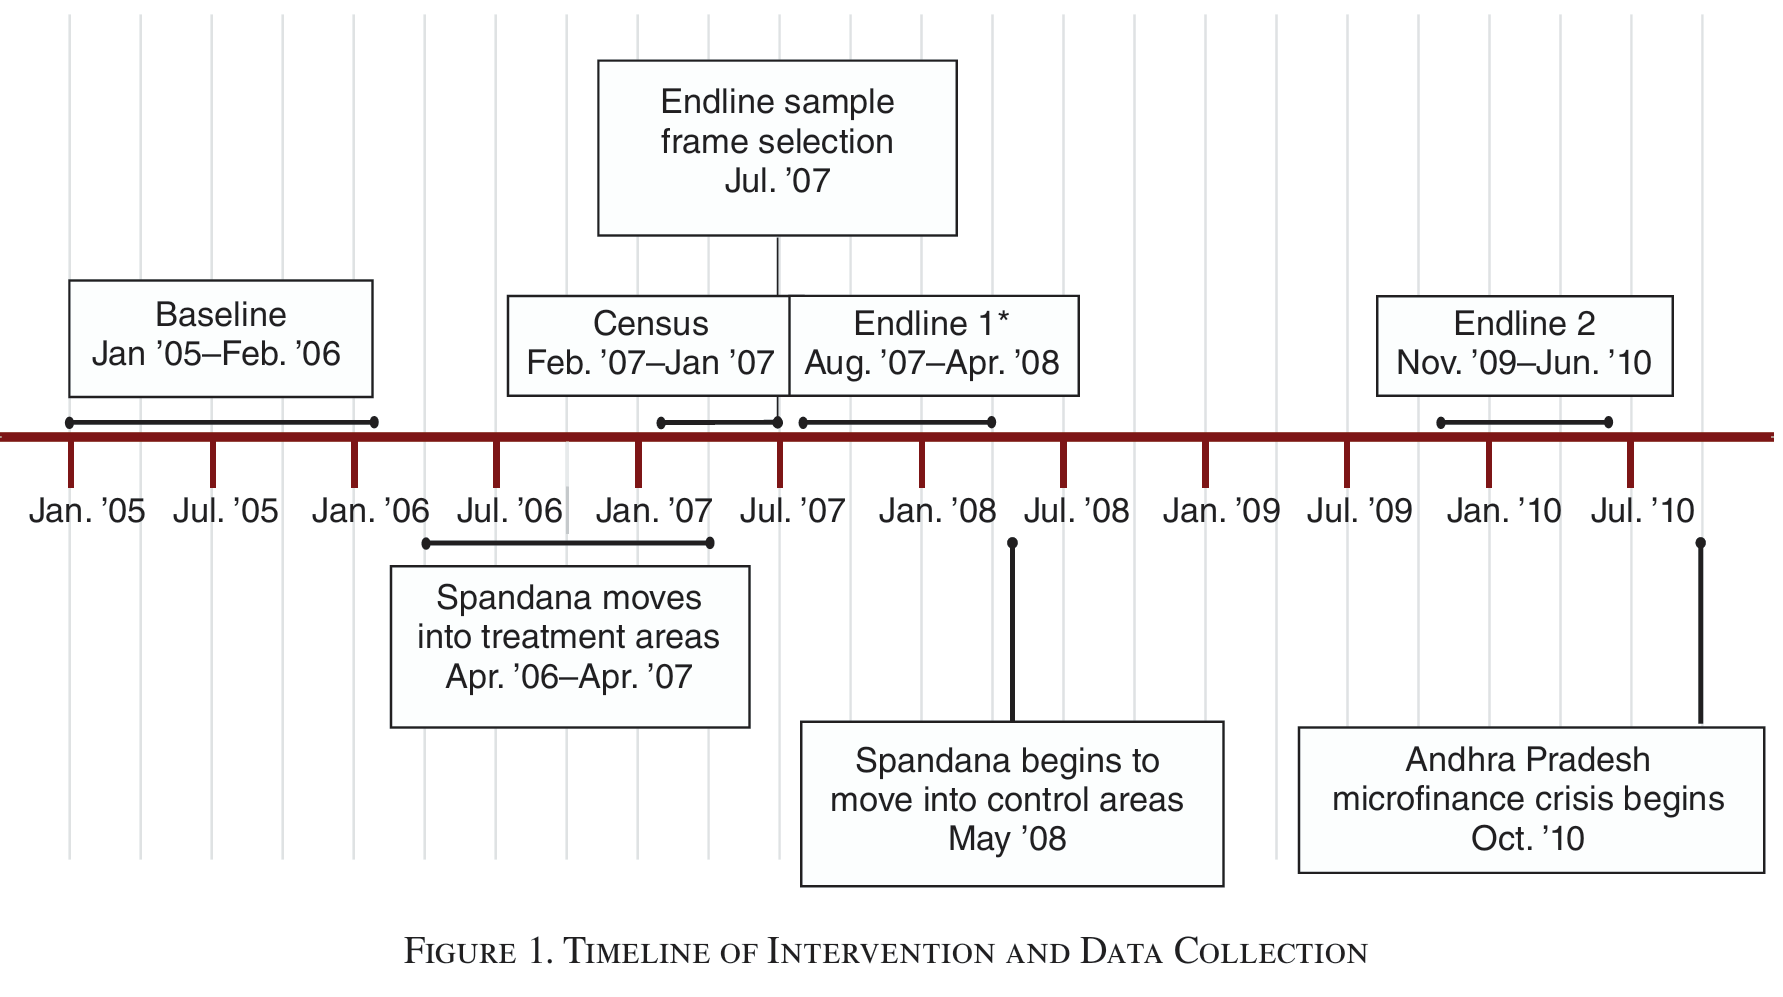
\includegraphics{Images/Banerjee_Timeline_1.png}

\begin{itemize}
\tightlist
\item
  Outcomes of interest:
\end{itemize}

\begin{enumerate}
\def\labelenumi{\arabic{enumi}.}
\tightlist
\item
  consumption
\item
  business creation
\item
  business income
\item
  education
\item
  health
\item
  women's empowerment
\end{enumerate}

\begin{itemize}
\item
  Initial (18-month) take-up is lower than expected (by Spandana):
  26.7\% in treated neighbourhoods and 18.3\% in control.
\item
  NOTE: control group is not `untreated' as other companies enter both
  treated and control groups during this period.

  \par

  \begin{itemize}
  \tightlist
  \item
    By second survey both groups had similar take-up, but treatment
    group had bigger and older loans.
  \end{itemize}
\item
  Highlights after 18 months:

  \par

  \begin{enumerate}
  \def\labelenumi{\arabic{enumi}.}
  \tightlist
  \item
    Decline in informal borrowing. 2. No difference in borrowed amount.
    3. No difference in (nondurable) consumption, but increase in
    purchase of durable goods. 4. No impact on entrepreneurship, but
    invest in existing businesses. 5. Increase in profitability of some
    businesses (upper tail)
  \end{enumerate}
\item
  Highlights after 42 months:

  \par

  \begin{enumerate}
  \def\labelenumi{\arabic{enumi}.}
  \tightlist
  \item
    Businesses have more assets, more businesses are more profitable 2.
    Average still small \(\Rightarrow\) doesn't help small businesses 3.
    No evidence of consumption change
  \end{enumerate}
\item
  No effect on female empowerment outcomes.
\item
  Almost 70\% of households do not have an MFI loan, despite
  eligibility, yet borrow from other sources.
\end{itemize}

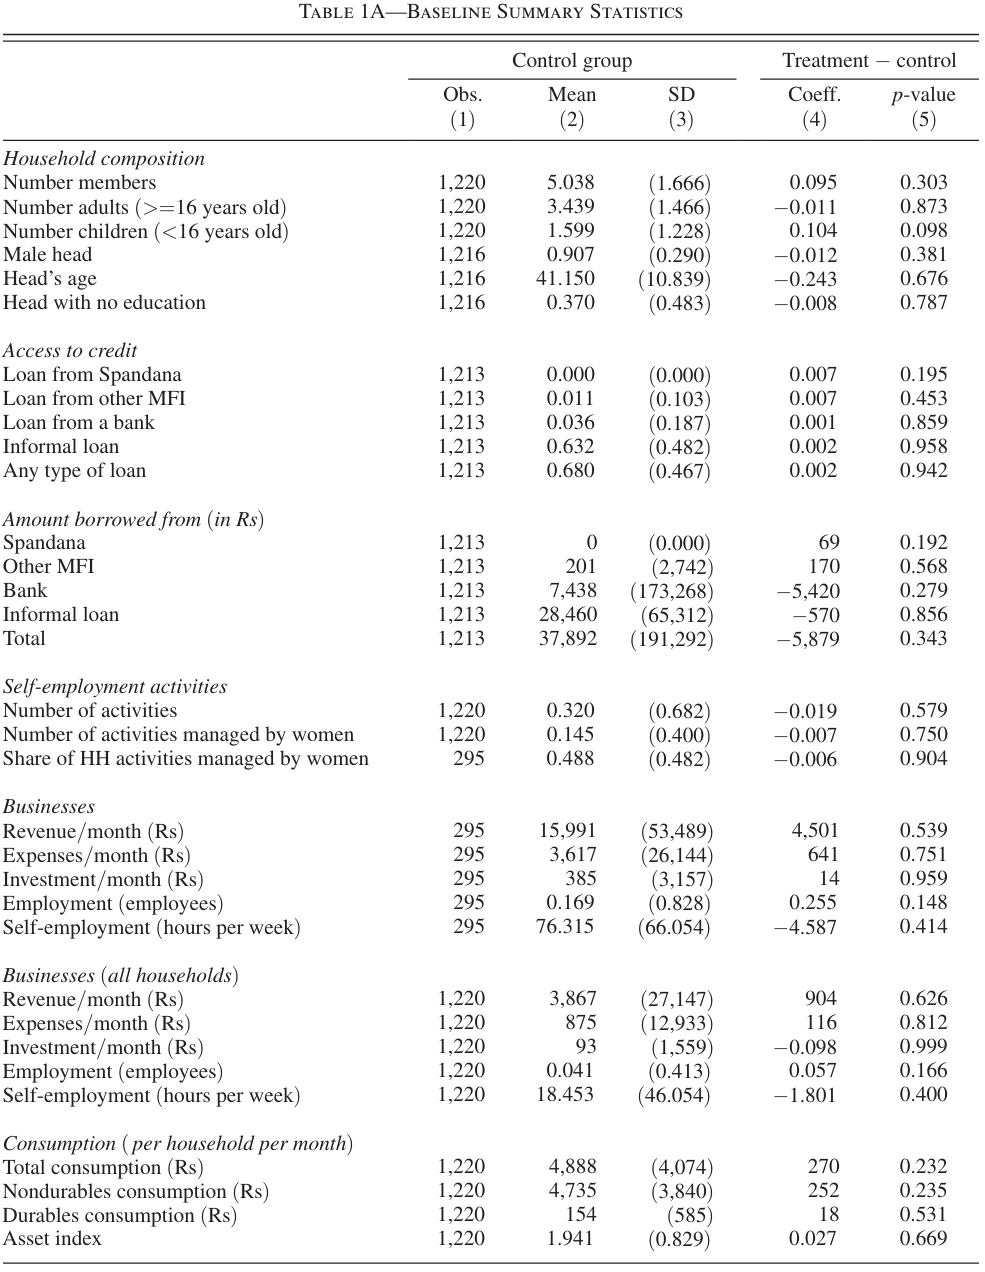
\includegraphics{Images/Banerjee_Baseline_1.png}

NOTE: Baseline survey covers a different set of households.

The authors estimate the following regression model in each period after
the intervention,\footnote{I have use the authors' notation.}

\[
            y_{ia} = \alpha + \beta \times Treat_{ia} + X_a'\gamma + \varepsilon_{ia}
\]

where \(i\) represents the individual and \(a\) the area
(neighbourhood).

\par

\begin{itemize}
\tightlist
\item
  \(X_a\) is a vector of area controls \textbf{at baseline}, including
  population, per capita literature, etc.
\end{itemize}

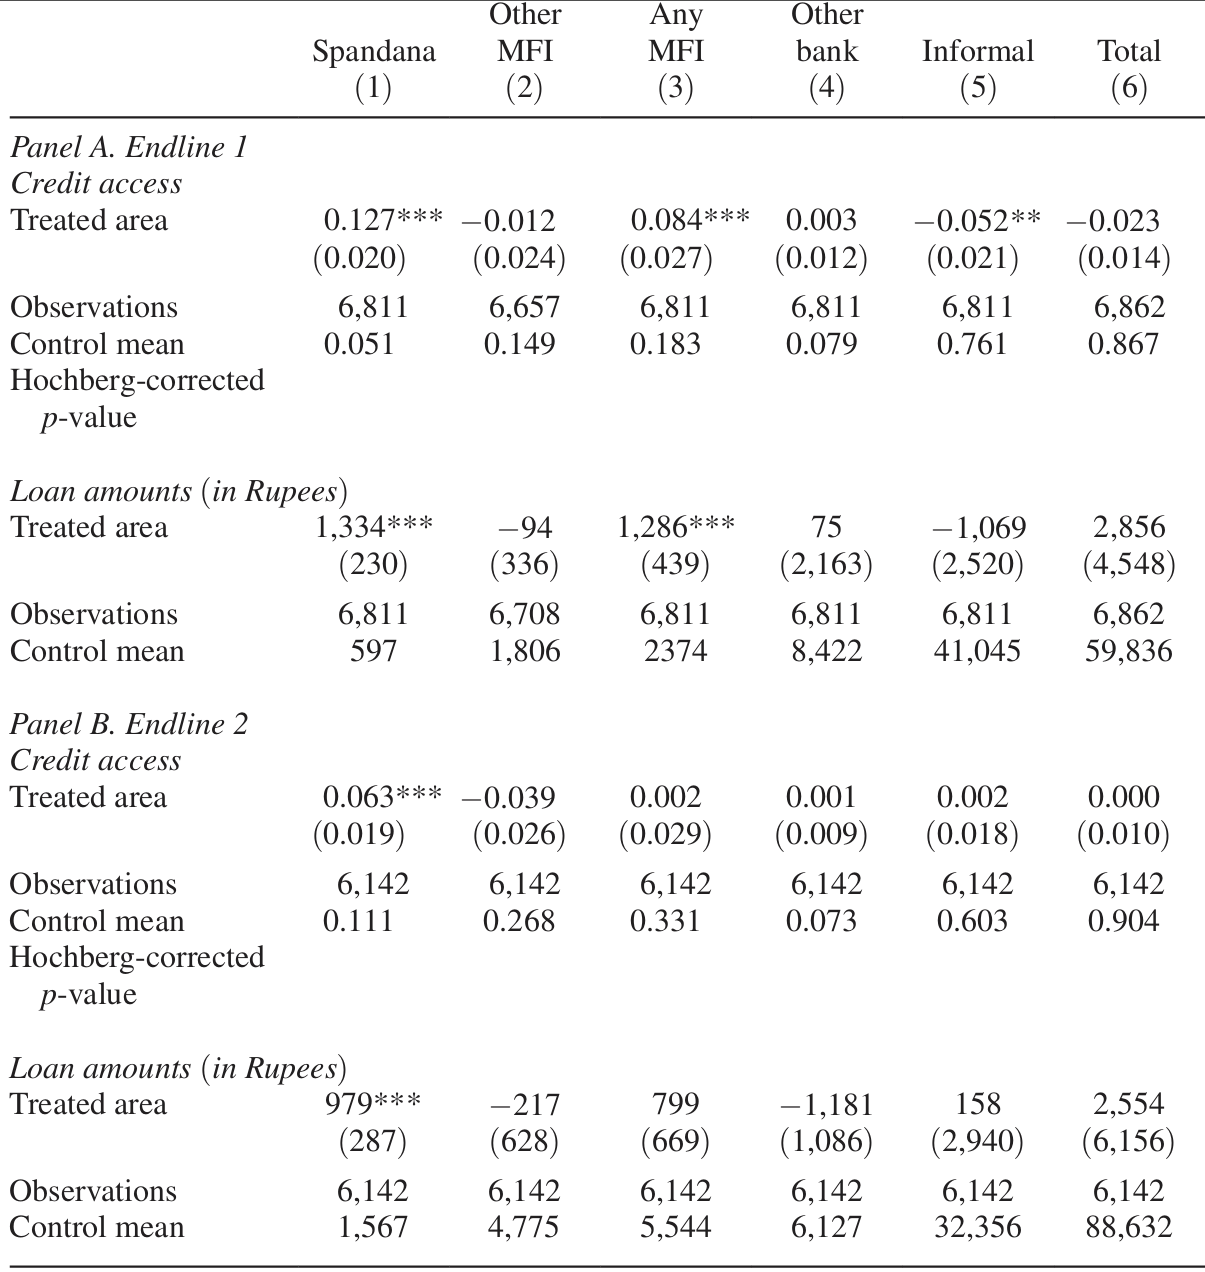
\includegraphics{Images/Banerjee_Regression_1.png}
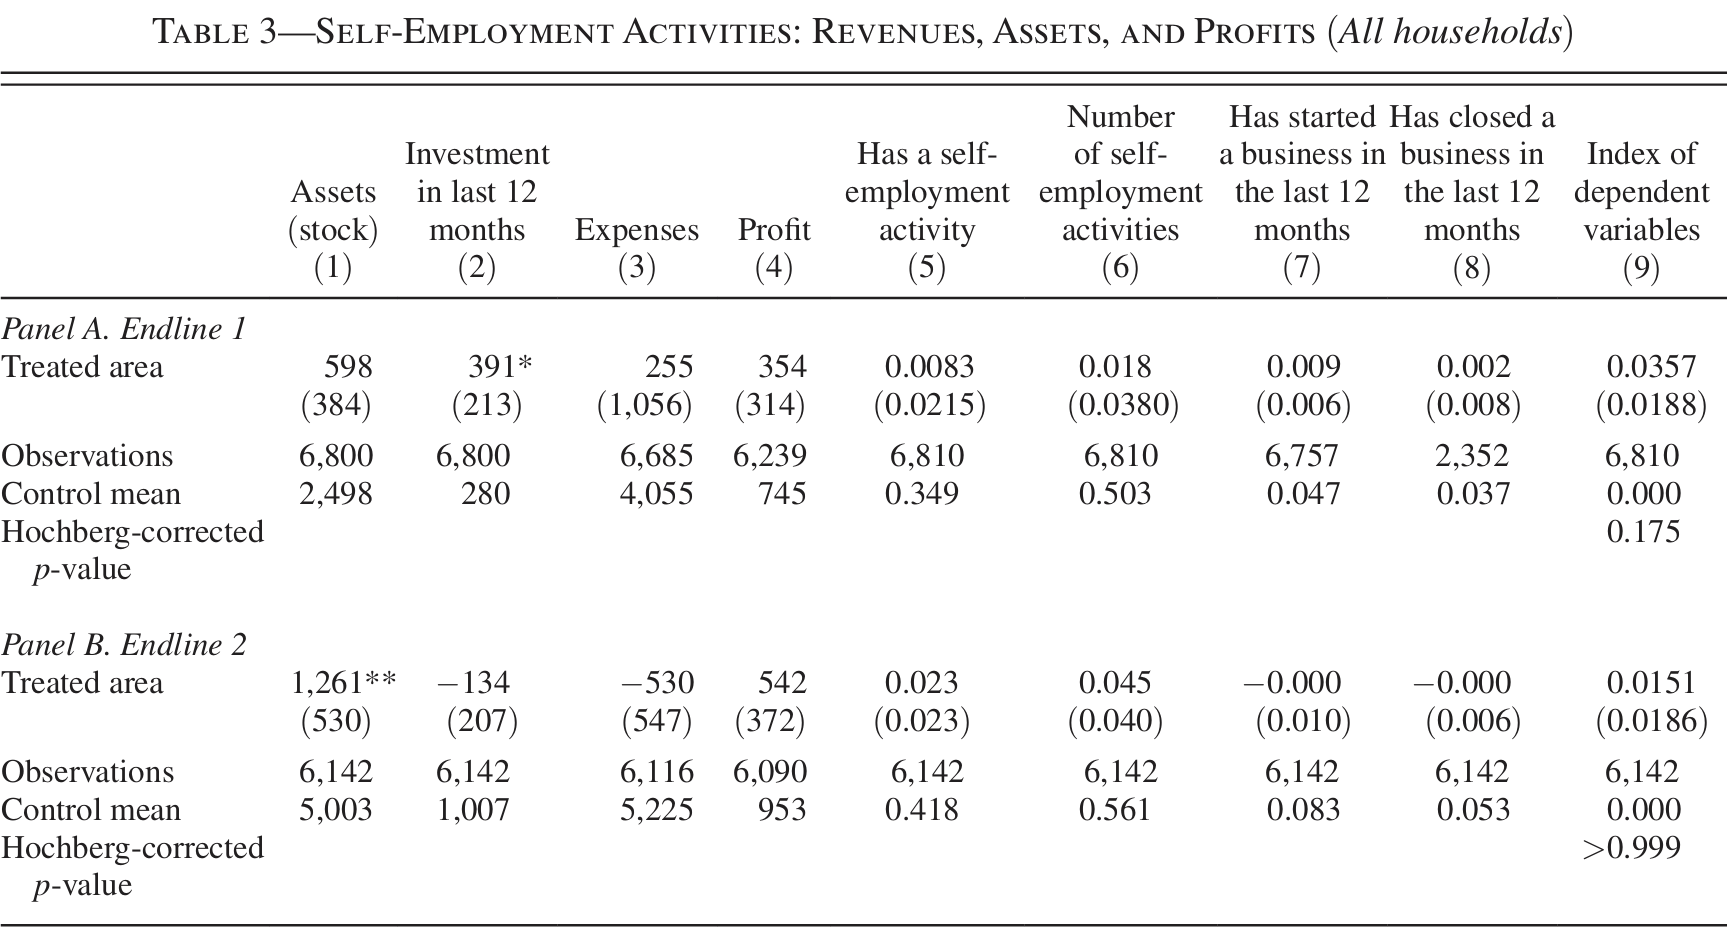
\includegraphics{Images/Banerjee_Regression_3.png}
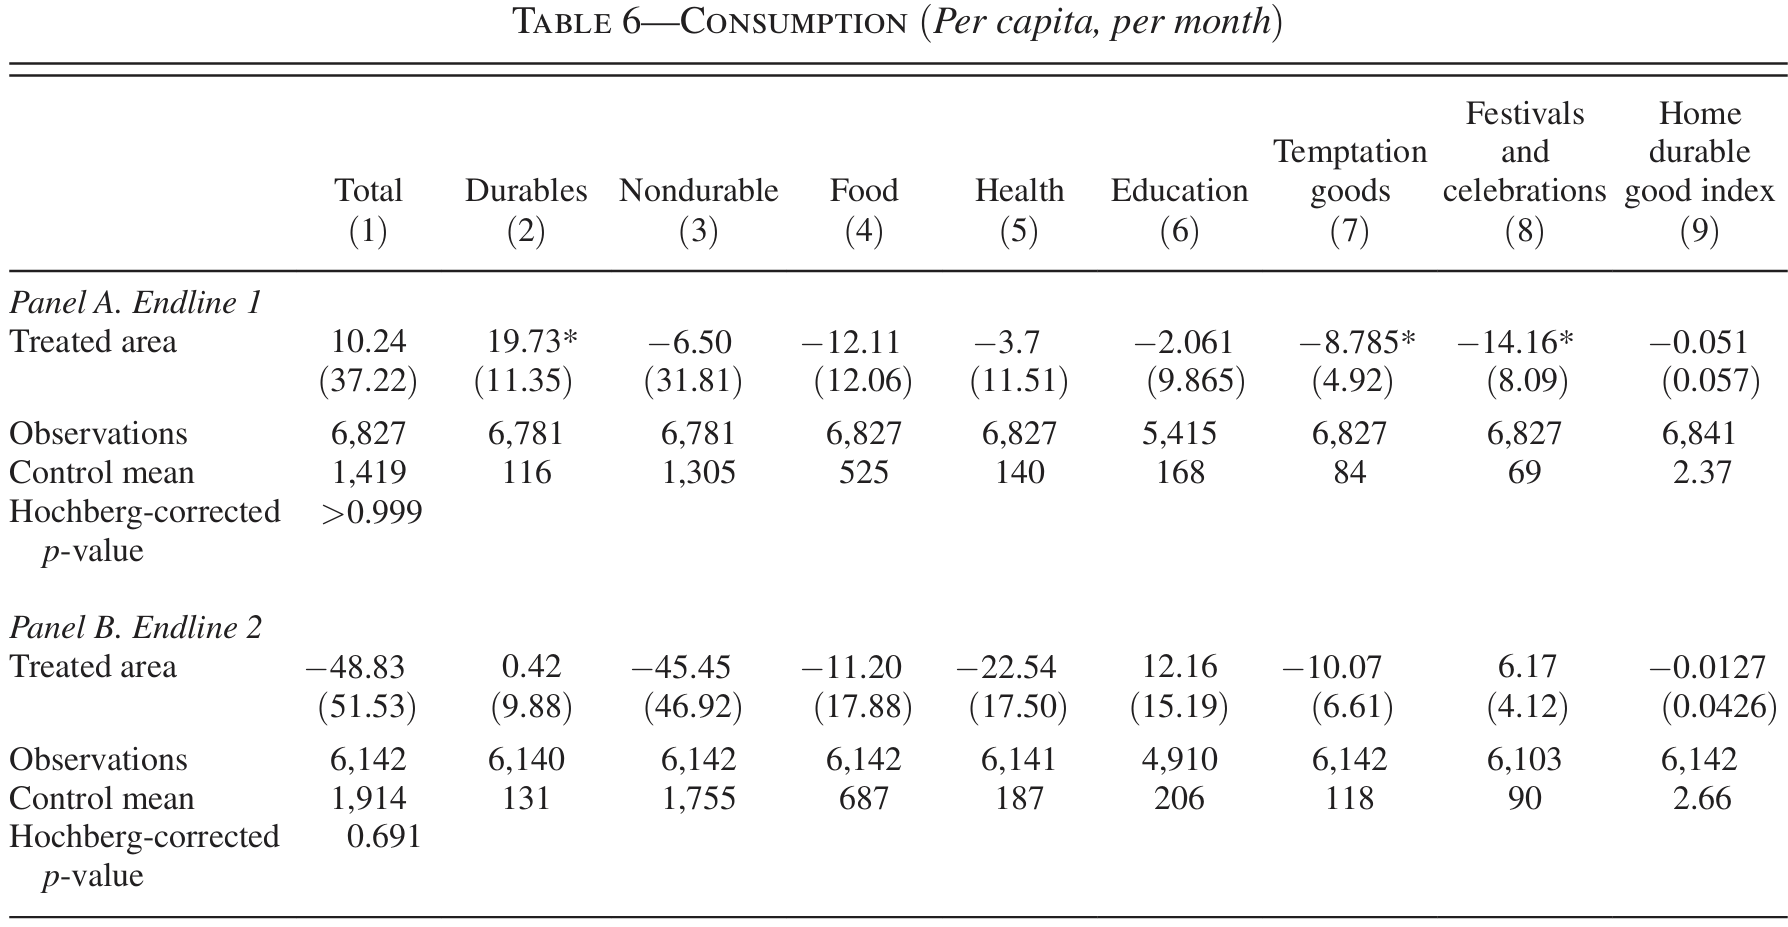
\includegraphics{Images/Banerjee_Regression_2.png}

Conclusion:

\emph{``microcredit is not for every household, or even most households,
and \textbf{it does not lead to the miraculous social transformation}
some proponents have claimed\ldots allows some households to sacrifice
some instantaneous utility (temptation goods or leisure) in order to
finance lumpy purchases, either for their home or in order to establish
or expand a business''}

Similar results found in other RCTs, including ``Estimating the impact
of microcredit on those who take it up: Evidence from a randomized
experiment in Morocco'\,' by Cr'\{e\}pon, Devoto, Duflo \& Parient'\{e\}
(2015)

\par

\begin{itemize}
\tightlist
\item
  Clearer research design with untreated control group
\item
  No evidence of a gain in income or consumption
\end{itemize}

\subsubsection{Notes on sample variance (in
R)}\label{notes-on-sample-variance-in-r}

\begin{Shaded}
\begin{Highlighting}[]
\NormalTok{data1 }\OtherTok{\textless{}{-}}\FunctionTok{data.frame}\NormalTok{(}\AttributeTok{y0 =} \FunctionTok{c}\NormalTok{(}\DecValTok{1}\NormalTok{,}\DecValTok{3}\NormalTok{,}\DecValTok{2}\NormalTok{,}\DecValTok{4}\NormalTok{),}
\AttributeTok{y1 =} \FunctionTok{c}\NormalTok{(}\DecValTok{3}\NormalTok{,}\DecValTok{1}\NormalTok{,}\DecValTok{3}\NormalTok{,}\DecValTok{3}\NormalTok{)}
\NormalTok{)}
\NormalTok{data1}\SpecialCharTok{$}\NormalTok{tau }\OtherTok{\textless{}{-}}\NormalTok{  data1}\SpecialCharTok{$}\NormalTok{y1}\SpecialCharTok{{-}}\NormalTok{data1}\SpecialCharTok{$}\NormalTok{y0}
\NormalTok{data1}\SpecialCharTok{$}\NormalTok{St }\OtherTok{\textless{}{-}} \FunctionTok{c}\NormalTok{(}\FunctionTok{sd}\NormalTok{(data1}\SpecialCharTok{$}\NormalTok{y1)}\SpecialCharTok{\^{}}\DecValTok{2}\NormalTok{,}\FunctionTok{sd}\NormalTok{(data1}\SpecialCharTok{$}\NormalTok{y0)}\SpecialCharTok{\^{}}\DecValTok{2}\NormalTok{,}\FunctionTok{sd}\NormalTok{(data1}\SpecialCharTok{$}\NormalTok{tau)}\SpecialCharTok{\^{}}\DecValTok{2}\NormalTok{,}\ConstantTok{NA}\NormalTok{)}
\FunctionTok{print}\NormalTok{(}\FunctionTok{paste}\NormalTok{(}\StringTok{"Finite Sample Variance Tau{-}hat:"}\NormalTok{, data1}\SpecialCharTok{$}\NormalTok{St[}\DecValTok{1}\NormalTok{]}\SpecialCharTok{/}\DecValTok{2}\SpecialCharTok{+}\NormalTok{data1}\SpecialCharTok{$}\NormalTok{St[}\DecValTok{2}\NormalTok{]}\SpecialCharTok{/}\DecValTok{2}\SpecialCharTok{{-}}\NormalTok{data1}\SpecialCharTok{$}\NormalTok{St[}\DecValTok{3}\NormalTok{]}\SpecialCharTok{/}\DecValTok{4}\NormalTok{))}
\end{Highlighting}
\end{Shaded}

\begin{verbatim}
[1] "Finite Sample Variance Tau-hat: 0.5"
\end{verbatim}

Code out all the possible realizations of W

\begin{Shaded}
\begin{Highlighting}[]
\NormalTok{m }\OtherTok{\textless{}{-}} \DecValTok{1}
\ControlFlowTok{for}\NormalTok{ (i }\ControlFlowTok{in} \DecValTok{1}\SpecialCharTok{:}\DecValTok{3}\NormalTok{)\{}
\NormalTok{  j }\OtherTok{\textless{}{-}}\NormalTok{ i }\SpecialCharTok{+} \DecValTok{1}
  \ControlFlowTok{while}\NormalTok{ (j }\SpecialCharTok{\textless{}=} \DecValTok{4}\NormalTok{) \{}
\NormalTok{    data1[}\FunctionTok{paste0}\NormalTok{(}\StringTok{"w"}\NormalTok{, m)] }\OtherTok{\textless{}{-}} \FunctionTok{as.numeric}\NormalTok{((}\DecValTok{1}\SpecialCharTok{:}\FunctionTok{nrow}\NormalTok{(data1) }\SpecialCharTok{==}\NormalTok{ i) }\SpecialCharTok{|}\NormalTok{ (}\DecValTok{1}\SpecialCharTok{:}\FunctionTok{nrow}\NormalTok{(data1) }\SpecialCharTok{==}\NormalTok{ j))}
\NormalTok{    m }\OtherTok{\textless{}{-}}\NormalTok{ m }\SpecialCharTok{+} \DecValTok{1}
\NormalTok{    j }\OtherTok{\textless{}{-}}\NormalTok{ j }\SpecialCharTok{+} \DecValTok{1}
\NormalTok{  \}}
\NormalTok{\}}

\NormalTok{tauhat }\OtherTok{\textless{}{-}} \FunctionTok{matrix}\NormalTok{(}\ConstantTok{NA}\NormalTok{, }\AttributeTok{nrow =} \DecValTok{6}\NormalTok{, }\AttributeTok{ncol =} \DecValTok{1}\NormalTok{)}

\ControlFlowTok{for}\NormalTok{ (i }\ControlFlowTok{in} \DecValTok{1}\SpecialCharTok{:}\DecValTok{6}\NormalTok{) \{}
\NormalTok{  data1[}\FunctionTok{paste0}\NormalTok{(}\StringTok{"yobs"}\NormalTok{, i)] }\OtherTok{\textless{}{-}}\NormalTok{ data1}\SpecialCharTok{$}\NormalTok{y1 }\SpecialCharTok{*}\NormalTok{ data1[}\FunctionTok{paste0}\NormalTok{(}\StringTok{"w"}\NormalTok{, i)] }\SpecialCharTok{+}\NormalTok{ data1}\SpecialCharTok{$}\NormalTok{y0 }\SpecialCharTok{*}\NormalTok{ (}\DecValTok{1} \SpecialCharTok{{-}}\NormalTok{ data1[}\FunctionTok{paste0}\NormalTok{(}\StringTok{"w"}\NormalTok{, i)])}
\NormalTok{  model }\OtherTok{\textless{}{-}} \FunctionTok{lm}\NormalTok{(}\FunctionTok{paste0}\NormalTok{(}\StringTok{"yobs"}\NormalTok{, i, }\StringTok{" \textasciitilde{} "}\NormalTok{, }\StringTok{"w"}\NormalTok{, i), }\AttributeTok{data =}\NormalTok{ data1)}
\NormalTok{  tauhat[i, }\DecValTok{1}\NormalTok{] }\OtherTok{\textless{}{-}} \FunctionTok{coef}\NormalTok{(model)[}\FunctionTok{paste0}\NormalTok{(}\StringTok{"w"}\NormalTok{, i)]}
\NormalTok{\}}
\FunctionTok{print}\NormalTok{(}\FunctionTok{paste0}\NormalTok{(}\StringTok{"Finite Sample Variance Tau{-}hat is "}\NormalTok{, }\FunctionTok{sd}\NormalTok{(tauhat)}\SpecialCharTok{\^{}}\DecValTok{2}\SpecialCharTok{*}\DecValTok{5}\SpecialCharTok{/}\DecValTok{6}\NormalTok{))}
\end{Highlighting}
\end{Shaded}

\begin{verbatim}
[1] "Finite Sample Variance Tau-hat is 0.5"
\end{verbatim}

\chapter{Stratified Experiments}\label{sec-stratified}

The discussion of simple randomized experiments ignores the possibility
that assignment into treatment depends on an set of covariates \(X_i\).
In this chapter we discuss experimental designs where the probability of
treatment is stratified on characteristics of unit.

Stratification is used to support the within-group analysis of
experiments and can have significant benefits for the statistical power
of the causal effects estimator. Stratified experiments will also form
the basis of the way in which researchers think about casual inference
using (cross-sectional) observational data where selection into
treatment is not controlled (see Chapter \_).

\subsection{Stratified Randomized
Experiment}\label{stratified-randomized-experiment}

Stratification involves the dividing of the population into a finite
number of \textbf{blocks} or \textbf{strata} (\(B_i \in \{1,...,J\}\)),
based on \emph{pre-treatment}, observable characteristics \(X_i\),

\[
B_i = B_i(X_i)
\]

Within each block, assignment into treatment is both probabilistic and
individual, but differs by \(X_i\). Thus, there is a completely
randomized experiment within each block and assignment is independent
across blocks.

Adapting our original definition of a completely randomized experiment
(from Chapter \_) to this setting, we get that the probability of
observing any assignment vector \(W_i\) conditional on potential
outcomes and a vecotr of \(X_i\)-covariates is given by,

\[
\mathbf{Pr}(W|X,Y(0),Y(1))=
\begin{cases}
\prod^J_{j=1} (\frac{N(j)!}{N(j)_t!(N(j)-N(j)_t)!})^{-1} & \text{if} \quad \sum^N_{i:B_i=j} W_i=N(j)_t \\
                    0 &\text{otherwise}
\end{cases}
\] and \$N(j)\_c is preset such that,

\[
0 < N(j)_t <N(j) \quad \text{for} \space j = 1,...,J
\]

Note, if N(j) \#\#\# Def. Stratified Randomized Experiment

\chapter{Irregular Assignment}\label{sec-regular}

This is a book created from markdown and executable code.

See Knuth (1984) for additional discussion of literate programming.

\begin{Shaded}
\begin{Highlighting}[]
\DecValTok{1} \SpecialCharTok{+} \DecValTok{1}
\end{Highlighting}
\end{Shaded}

\begin{verbatim}
[1] 2
\end{verbatim}

\part{Observational Studies}

\chapter{Propensity Score}\label{propensity-score}

\begin{tcolorbox}[enhanced jigsaw, bottomrule=.15mm, coltitle=black, arc=.35mm, left=2mm, opacityback=0, leftrule=.75mm, colbacktitle=quarto-callout-note-color!10!white, title={Def. Finite Population Propensity Score}, toprule=.15mm, bottomtitle=1mm, breakable, colframe=quarto-callout-note-color-frame, opacitybacktitle=0.6, titlerule=0mm, colback=white, rightrule=.15mm, toptitle=1mm]

The propensity score at \(x\) is the average unit assignment probability
for units with \(X_i = x\) \[
e(x)=\frac{1}{N(x)} \sum_{i=1} p_i(X,Y(0),Y(1))
\]

\end{tcolorbox}

\begin{tcolorbox}[enhanced jigsaw, bottomrule=.15mm, coltitle=black, arc=.35mm, left=2mm, opacityback=0, leftrule=.75mm, colbacktitle=quarto-callout-note-color!10!white, title={Def. Unit Assignment Probability}, toprule=.15mm, bottomtitle=1mm, breakable, colframe=quarto-callout-note-color-frame, opacitybacktitle=0.6, titlerule=0mm, colback=white, rightrule=.15mm, toptitle=1mm]

The probability that unit \(i\) is assigned to treatment, \[
p_i(X,Y(0),Y(1)) = \sum_{W:W_i=1}\mathbf{Pr}(W|X,Y(0),Y(1))
\]

\end{tcolorbox}

In a completely randomized experiment, \[
e(X_i)=\frac{N_t}{N}
\] i.e.~equal for all units and independent of \(X_i\)

\chapter{Observational Studies}\label{observational-studies-1}

\chapter{\texorpdfstring{The CEF (of \(Y(0)\))
Approach}{The CEF (of Y(0)) Approach}}\label{the-cef-of-y0-approach-1}

\section{CEF Approach}\label{cef-approach-1}

The shortcut approach to the identification of causal effects with
linear regression involves:

\begin{itemize}
\item
  \textbf{CEF of} \(Y_i(0)\): Assume \[
  E[Y_i(0)|X_i'] = X_i'\gamma
  \] This may include a constant term.
\item
  \textbf{Additive treatment effects}: \[
  Y_i(1) = Y_i(0) + \tau_i
  \]
\item
  \textbf{Heterogeneity independent of} \(X\)'s: \[
  E[Y_i(1) - Y_i(0)|D_i,X_i'] = E[Y_i(1) - Y_i(0)|D_i]
  \]
\end{itemize}

We do need to assume an additional assumption concerning assignment:

\begin{itemize}
\item
  \textbf{CIA/Unconfoundedness}: \[
  (Y(1),Y(0)) \perp D | X
  \]

  \textbf{or} a weaker,
\item
  \textbf{Unconfoundedness for controls}: \[
  Y(0) \perp D | X
  \]
\end{itemize}

While we have defined \(E[Y_i(0)|X_i']\), the linear regression model
will depend on:

\[
\begin{aligned}
E[Y^{obs}_i|D_i,X_i'] &= E[Y_i(0)+\tau_iD_i|D_i,X_i'] \\
                      &= E[Y_i(0)|D_i,X_i']+E[\tau_iD_i|D_i,X_i'] \\
                      &= E[Y_i(0)|X_i']+E[Y_i(1)-Y_i(0)|D_i]D_i \\
                      &= X_i'\gamma + E[Y_i(1)-Y_i(0)|D_i]D_i
\end{aligned}
\]

From line 2 to 3, \[
E[Y_i(0)|D_i,X_i'] = E[Y_i(0)|X_i']
\] holds if either confoundedness assumptions hold.

If we assume the stronger CIA-unconfoundedness, \[
E[Y_i(1)-Y_i(0)|D_i]D_i = E[Y_i(1)-Y_i(0)]D_i = \tau_{\scriptsize{ATE}}D_i
\] This gives us the CEF, \[
E[Y^{obs}_i|D_i,X_i'] = \tau_{\scriptsize{ATE}}D_i + X_i'\gamma
\]

If we assume the weaker unconfoundedness for covariates assumption, \[
E[Y_i(1)-Y_i(0)|D_i]D_i = \left(\tau_{ATU} + D_i(\tau_{ATT}-\tau_{ATU})\right)D_i = \tau_{ATT}D_i
\]

This gives us the CEF, \[
E[Y^{obs}_i|D_i,X_i'] = \tau_{ATT}D_i + X_i'\gamma
\]

By specifying the CEF of both \(Y_i(1)\) and \(Y_i(0)\), we know that \[
Y^{obs}_i = \tau_{ATT}D_i + X_i'\gamma + \varepsilon_i
\] where, \[
E[\varepsilon_i|D_i,X_i'] = 0
\]

By specifying the CEF of both \(Y_i(1)\) and \(Y_i(0)\), we understand
that:

\begin{itemize}
\tightlist
\item
  There is no question whether the linear regression model gives us the
  ATE/ATT.
\item
  This is a fairly strong assumption and not in the spirit of the RCT
  approach.
\item
  When examining RCTs, we were agnostic about the CEF.
\end{itemize}

\section{CEF Approach}\label{cef-approach-2}

One crucial omission from this approach is that we do not need to assume
overlap (or common support).

\textbf{Overlap}: \[
0 < e(X_i) < 1
\] where, \(e(X_i) = Pr(W_i=1|X_i')\)

\textbf{Interpretation}: The correctly specified CEF allows us to
perfectly predict the unobserved counterfactual of treated individuals
based on their \(X_i\). With unconfoundedness (for covariates), we can
estimate this counterfactual using the control group.

\chapter{The CIA Approach}\label{the-cia-approach}

\section{Conditional Independence
Assumption}\label{conditional-independence-assumption}

As with completely random experiments, we can achieve identification of
TE's via unconfoundedness.

\textbf{Conditional Independence Assumption (CIA)}: \[
(Y_i(1), Y_i(0)) \perp D_i | X_i'
\] ``When treatment and outcome variables can be considered to be
independent of one another after conditioning on control variables''
(Wooldridge, 2010, p.799)\footnote{CIA is the name used by Angrist and
  Pischke in MM and MHE when referring to unconfoundedness.}

The CIA implies: \[
\begin{aligned}
E[Y_i|D_i=1,X_i'] - E[Y_i|D_i=0,X_i'] &= E[Y_i(1)|D_i=1,X_i'] - E[Y_i(0)|D_i=0,X_i'] \\
&= E[Y_i(1)|X_i'] - E[Y_i(0)|X_i'] \\
&= E[Y_i(1) - Y_i(0)|X_i']
\end{aligned}
\]

CIA rules out selection, conditional on observables:

\textbf{Selection on observables}: Under CIA, \[
E[Y_i(0)|D_i=1,X_i'] - E[Y_i(0)|D_i=0,X_i'] = 0
\]

This rules out selection on unobservables.

Two remaining questions: 1. How should we compute these
covariate-matched treatment effects? 2. What are the relevant
covariates?

\section{Common Support}\label{common-support}

Crucially, we now need to assume common support (or overlap):

\textbf{Overlap}: \[
0 < e(X_i) < 1
\] where, \(e(X_i) = Pr(W_i=1|X_i')\)

\section{Conditional ATE}\label{conditional-ate}

Suppose we had a single covariate that took on \(m\) \textbf{finite}
values:

\[
X_i \in \{x_1, x_2, \ldots, x_m\}
\]

\textbf{Under CIA,}

\[
E[Y_i|D_i=1, X_i=x_k] - E[Y_i|D_i=0, X_i=x_k] = \tau_{\scriptsize{ATE}}(x_k)
\]

\section[ATE as a Weighted Average]{\texorpdfstring{ATE as a Weighted
Average\footnote{Here I borrow from Abadie and Cattaneo (2018), which is
  on Moodle.}}{ATE as a Weighted Average}}\label{ate-as-a-weighted-averagecef-2}

\textbf{Under CIA}, we can define the superpopulation ATE as:

\[
\tau_{\scriptsize{ATE}} = \sum_{k=1}^{m} \left(E[Y_i|D_i=1, X_i=x_k] - E[Y_i|D_i=0, X_i=x_k]\right)Pr(X_i=x_k)
\]

Likewise, we can define the ATT as:

\[
\tau_{ATT} = \sum_{k=1}^{m} \left(E[Y_i|D_i=1, X_i=x_k] - E[Y_i|D_i=0, X_i=x_k]\right)Pr(X_i=x_k|D_i=1)
\]

\chapter{Regression as Matching}\label{regression-as-matching}

\textbf{Regression as Matching}\footnote{This result is also
  demonstrated in MHE.}

We could then consider estimating these treatment effects using the
linear regression model\footnote{This is often referred to as a
  \emph{fully saturated} regression.}:

\[
Y_i = \beta D_i + \sum_{k=1}^{m} \gamma_k \mathbf{1}\{X_i=x_k\} + \upsilon_i
\]

It can be shown that:

\[
\beta = \sum_{k=1}^{m} \left(E[Y_i|D_i=1, X_i=x_k] - E[Y_i|D_i=0, X_i=x_k]\right)w_k
\]

where:

\[
w_k = \frac{Var(D_i|X_i=x_k)Pr(X_i=x_k)}{\sum_{j=1}^{m} Var(D_i|X_i=x_j)Pr(X_i=x_j)}
\]

The linear regression model coefficient is a \textbf{variance-weighted}
average of the conditional mean differences. The weights depend on the
variance of \(D_i\) conditional on \(X_i\) and more weight will be
applied to cases where the treatment allocation is equal (50-50).

Thus,

\[
\beta \neq \tau_{\scriptsize{ATE}}
\]

unless
\(\tau_{\scriptsize{ATE}}(x_k) = \tau_{\scriptsize{ATE}} \quad \forall \; k=1, \ldots, m\);
since the weights sum to 1. This is NOT the same as homogeneous
treatment effects.

\chapter{Conditional ATE}\label{conditional-ate-1}

Suppose we have a single covariate that takes on \(m\) \textbf{finite}
values:

\[
X_i \in \{x_1, x_2, \ldots, x_m\}
\]

\textbf{Under CIA}:

\[
E[Y_i | D_i = 1, X_i = x_k] - E[Y_i | D_i = 0, X_i = x_k] = \tau_{\scriptsize{ATE}}(x_k)
\]

\chapter[ATE as a Weighted Average]{\texorpdfstring{ATE as a Weighted
Average\footnote{Here I borrow from Abadie and Cattaneo (2018), which is
  on Moodle}}{ATE as a Weighted Average}}\label{ate-as-a-weighted-averagecef-5}

\textbf{Under CIA}, we can define the super population ATE as:

\[
\tau_{\scriptsize{ATE}} = \sum_{k=1}^{m} \left( E[Y_i | D_i = 1, X_i = x_k] - E[Y_i | D_i = 0, X_i = x_k] \right) Pr(X_i = x_k)
\]

Likewise, we can define the ATT as:

\[
\tau_{ATT} = \sum_{k=1}^{m} \left( E[Y_i | D_i = 1, X_i = x_k] - E[Y_i | D_i = 0, X_i = x_k] \right) Pr(X_i = x_k | D_i = 1)
\]

\chapter{Regression as Matching}\label{regression-as-matching-1}

\textbf{Regression as Matching}\footnote{This result is also
  demonstrated in MHE}

We could then consider estimating these treatment effects using the
linear regression model\footnote{This is often referred to as a
  \emph{fully saturated} regression.}:

\[
Y_i = \beta D_i + \sum_{k=1}^{m} \gamma_k \mathbf{1} \{X_i = x_k\} + \upsilon_i
\]

It can be shown that:

\[
\beta = \sum_{k=1}^{m} \left( E[Y_i | D_i = 1, X_i = x_k] - E[Y_i | D_i = 0, X_i = x_k] \right) w_k
\]

where:

\[
w_k = \frac{Var(D_i | X_i = x_k) Pr(X_i = x_k)}{\sum_{j=1}^{m} Var(D_i | X_i = x_j) Pr(X_i = x_j)}
\]

The linear regression model coefficient is a \textbf{variance-weighted}
average of the conditional mean differences. The weights:

\begin{itemize}
\tightlist
\item
  Depend on the variance of \(D_i\) conditional on \(X_i\).
\item
  More weight will be applied to cases where the treatment allocation is
  equal (50-50).
\end{itemize}

Thus:

\[
\beta \neq \tau_{\scriptsize{ATE}}
\]

\textbf{Unless}
\(\tau_{\scriptsize{ATE}}(x_k) = \tau_{\scriptsize{ATE}} \quad \forall \; k = 1, \ldots, m\);
since the weights sum to 1. This is \textbf{NOT} the same as homogeneous
treatment effects.

\chapter{Next-up}\label{next-up-1}

\begin{enumerate}
\def\labelenumi{\arabic{enumi}.}
\tightlist
\item
  Propensity score matching
\item
  Picking covariates
\item
  Selection on \textbf{un}observables
\end{enumerate}

Other topics:

\begin{itemize}
\tightlist
\item
  Continuous treatment
\end{itemize}

Appendices with proofs and additional theorems can follow similar
markdown structuring for their inclusion.

\part{Natural Experiments}

\chapter{Eissa \& Liebman (1996)}\label{eissa-liebman-1996}

\begin{enumerate}
\def\labelenumi{\arabic{enumi}.}
\item
  Difference-in-Differences - Static

  Recall Lecture 1.2 \emph{Causal Inference},

  \section{(Imbens and Rubin, 2015,
  p.~6)}\label{imbens-and-rubin-2015-p.-6}

  \begin{enumerate}
  \def\labelenumii{\arabic{enumii}.}
  \tightlist
  \item
    ``First, the definition of the causal effect depends on the
    potential outcomes, but it does not depend on which outcome is
    actually observed.''
  \item
    ``Second, the causal effect is the comparison of potential outcomes,
    for the same unit, at the same moment in time post-treatment. In
    particular, \textbf{the causal effect is not defined in terms of
    comparisons of outcomes at different times.}\footnote{Emphasis
      added.}''
  \end{enumerate}

  \section{Set-up: 2-group-2-period}\label{set-up-2-group-2-period}

  The simple 2-group-2-period difference-in-differences set-up has the
  following characteristics,

  \begin{itemize}
  \tightlist
  \item
    Two periods of data: either panel (longitudinal) or repeated
    cross-section
  \item
    A control group that is never-treated\footnote{If you use an
      always-treated control group you would need to assume static
      treatment effects.}
  \item
    Treatment is absorbing: `always-on'\footnote{More relevant for
      multiple periods.}
  \item
    Typically, the treatment takes place in the second period.
  \end{itemize}

  Assuming additive treatment effects,

  \[
  Y_{it} = \begin{cases}
  Y_{it}(0) & \text{if } t < t_0 \\
  Y_{it}(0) + D_i\cdot(Y_{it}(1)-Y_{it}(0)) & \text{if } t \geq t_0
  \end{cases}
  \]

  \[
  = Y_{it}(0) + T_t\cdot D_i\cdot(Y_{it}(1)-Y_{it}(0))
  \]

  where, - ( \(T_t\) ): dummy variable ( \(=1\) ) after period of
  treatment (( \(t_0\) ) onwards). - ( \(D_i\) ): dummy variable (
  \(=1\) ) if unit ( \(i\) ) is in the treated group, 0 otherwise.

  \begin{tcolorbox}[enhanced jigsaw, bottomrule=.15mm, coltitle=black, arc=.35mm, left=2mm, opacityback=0, leftrule=.75mm, colbacktitle=quarto-callout-note-color!10!white, title={Note: ( \((Y_{it}(1),Y_{it}(0))\)) depend on time; so,}, toprule=.15mm, bottomtitle=1mm, breakable, colframe=quarto-callout-note-color-frame, opacitybacktitle=0.6, titlerule=0mm, colback=white, rightrule=.15mm, toptitle=1mm]

  \[
  Y_{it}(1)-Y_{it}(0) \lesseqqgtr Y_{it'}(1)-Y_{it'}(0)
  \]

  \end{tcolorbox}

  \section{Exclusion Restrictions}\label{exclusion-restrictions}

  The above set-up implies the following exclusion
  restrictions,\footnote{Particularly important in observational studies
    with group and/or irregular assignment.}

  \begin{tcolorbox}[enhanced jigsaw, bottomrule=.15mm, coltitle=black, arc=.35mm, left=2mm, opacityback=0, leftrule=.75mm, colbacktitle=quarto-callout-note-color!10!white, title={Exclusion restriction: No pre-emptive behaviour}, toprule=.15mm, bottomtitle=1mm, breakable, colframe=quarto-callout-note-color-frame, opacitybacktitle=0.6, titlerule=0mm, colback=white, rightrule=.15mm, toptitle=1mm]

  \[
  Y_{it}=Y_{it}(0) \quad \forall\; (i,t)\;\text{s.t. }\;t< t_0
  \]

  \end{tcolorbox}

  and,

  \begin{tcolorbox}[enhanced jigsaw, bottomrule=.15mm, coltitle=black, arc=.35mm, left=2mm, opacityback=0, leftrule=.75mm, colbacktitle=quarto-callout-note-color!10!white, title={Exclusion restriction: No spillovers}, toprule=.15mm, bottomtitle=1mm, breakable, colframe=quarto-callout-note-color-frame, opacitybacktitle=0.6, titlerule=0mm, colback=white, rightrule=.15mm, toptitle=1mm]

  \[
  Y_{it}=Y_{it}(0) \quad \forall \;(i,t) \;\text{s.t.}\;D_i=0
  \]

  \end{tcolorbox}

  and,

  \begin{tcolorbox}[enhanced jigsaw, bottomrule=.15mm, coltitle=black, arc=.35mm, left=2mm, opacityback=0, leftrule=.75mm, colbacktitle=quarto-callout-note-color!10!white, title={Exclusion restriction: No switching}, toprule=.15mm, bottomtitle=1mm, breakable, colframe=quarto-callout-note-color-frame, opacitybacktitle=0.6, titlerule=0mm, colback=white, rightrule=.15mm, toptitle=1mm]

  \textbf{Treatment group} status, \(D_i\), does not depend on time.
  Only treatment status, \(D_i \cdot T_t\), varies with time.

  \end{tcolorbox}

  \section{Dynamic Confounding
  Factors}\label{dynamic-confounding-factors}

  Let us consider the first (dynamic) difference with just \textbf{two
  periods of data},

  \[
  \begin{aligned}
  &E[Y_{it}|D_i=1,T_t=1]-E[Y_{it}|D_i=1,T_t=0] \\
  =&E[Y_{it}(1)|D_i=1,T_t=1]-E[Y_{it}(0)|D_i=1,T_t=0] \\
  =&\underbrace{E[Y_{it}(1)|D_i=1,T_t=1]-E[Y_{it}(0)|D_i=1,T_t=1]}_{\text{ATT in period } t_0} \\
  &\underbrace{+E[Y_{it}(0)|D_i=1,T_t=1]-E[Y_{it}(0)|D_i=1,T_t=0]}_{\text{(dynamic) confounding factors}}
  \end{aligned}
  \]

  Once again, we don't observe the counterfactual for the treated group.
  \textbf{As such}, the CEF does not trace out a causal relationship.

  Notice, however, that for the untreated group,

  \[
  \begin{aligned}
  &E[Y_{it}|D_i=0,T_t=1]-E[Y_{it}|D_i=0,T_t=0] \\
  =&E[Y_{it}(0)|D_i=0,T_t=1]-E[Y_{it}(0)|D_i=0,T_t=0]
  \end{aligned}
  \]

  which looks very similar to,

  \[
  \color{red}{E[Y_{it}(0)|D_i=1,T_t=1]}
  \] \[
  -E[Y_{it}(0)|D_i=1,T_t=0]
  \] (Note to myself: Find a way to change this)

  from the treated group.

  \begin{tcolorbox}[enhanced jigsaw, bottomrule=.15mm, coltitle=black, arc=.35mm, left=2mm, opacityback=0, leftrule=.75mm, colbacktitle=quarto-callout-note-color!10!white, title={Parallel Trends Assumption (General version)}, toprule=.15mm, bottomtitle=1mm, breakable, colframe=quarto-callout-note-color-frame, opacitybacktitle=0.6, titlerule=0mm, colback=white, rightrule=.15mm, toptitle=1mm]

  \[
  \begin{aligned}
  &E[Y_{it}(0)|D_i=0,T_t=1]-E[Y_{it}(0)|D_i=0,T_t=0] \\
  =&E[Y_{it}(0)|D_i=1,T_t=1]-E[Y_{it}(0)|D_i=1,T_t=0]
  \end{aligned}
  \]

  \end{tcolorbox}

  With this assumption and the above exclusion restrictions, we have
  identification of the Average Treatment Effect \textbf{of the
  Treated}.

  With this assumption we can identify the ATT,

  \[
  \begin{aligned}
  &\big[E[Y_{it}|D_i=1,T_t=1]-E[Y_{it}|D_i=1,T_t=0]\big]\\
  &-\big[\textcolor{blue}{E[Y_{it}|D_i=0,T_t=1]-E[Y_{it}|D_i=0,T_t=0]}\big] \\
  =&\big[E[Y_{it}(1)|D_i=1,T_t=1]-E[Y_{it}(0)|D_i=1,T_t=0]\big] \\
  &-\big[\textcolor{blue}{E[Y_{it}(0)|D_i=0,T_t=1]-E[Y_{it}(0)|D_i=0,T_t=0]}\big] \\
  =&\big[E[Y_{it}(1)|D_i=1,T_t=1]\textcolor{red}{-E[Y_{it}(0)|D_i=1,T_t=1]}\big] \\
  &+\big[\textcolor{red}{E[Y_{it}(0)|D_i=1,T_t=1]}-E[Y_{it}(0)|D_i=1,T_t=0]\big] \\
  &-\big[\textcolor{blue}{E[Y_{it}(0)|D_i=0,T_t=1]-E[Y_{it}(0)|D_i=0,T_t=0]}\big] \\
  =&\underbrace{\big[E[Y_{it}(1)|D_i=1,T_t=1]\textcolor{red}{-E[Y_{it}(0)|D_i=1,T_t=1]}\big]}_{\text{ATT in period } t_0}
  \end{aligned}
  \]

  where the two penultimate lines cancel one another under parallel
  trends. Hence, the name \textbf{difference-in-differences}.

  \section{Mapping to Linear Model}\label{mapping-to-linear-model}

  Let's consider the CEF of ( \(Y_{it}^{obs}\) ),

  \[
  E[Y_{it}|D_i,T_t]
  \]

  where, ( \(Y_{it} = Y_{it}(0) + T_t \cdot D_i(Y_{it}(1) - Y_{it}(0))\)
  ).\footnote{Remember, this equation implies our exclusion
    restrictions.}

  \[
  \begin{aligned}
  E[Y_{it}|D_i,T_t] &= E[Y_{it}(0)|D_i,T_t] + T_t \cdot D_i E[(Y_{it}(1) - Y_{it}(0))|D_i,T_t] \\
  &= E[Y_{it}(0)|D_i,T_t=0] \\
  &\quad + T_t \cdot \left( E[Y_{it}(0)|D_i,T_t=1] - E[Y_{it}(0)|D_i,T_t=0] \right) \\
  &\quad + T_t \cdot D_i \cdot E[(Y_{it}(1) - Y_{it}(0))|D_i,T_t]
  \end{aligned}
  \]

  \textbf{Under parallel trends},

  \[
  \begin{aligned}
  &E[Y_{it}(0)|D_i,T_t=1]-E[Y_{it}(0)|D_i,T_t=0] \\
  &= \textcolor{blue}{E[Y_{it}(0)|T_t=1]-E[Y_{it}(0)|T_t=0]} \\
  &= \textcolor{blue}{\delta}
  \end{aligned}
  \]

  a constant! So, we have

  \[
  \begin{aligned}
  E[Y_{it}|D_i,T_t] &= E[Y_{it}(0)|D_i,T_t=0] \\
  &+ T_t \cdot \left( \textcolor{blue}{\underbrace{E[Y_{it}(0)|T_t=1]-E[Y_{it}(0)|T_t=0]}_{\delta}} \right) \\
  &+ T_t \cdot D_i \cdot E[(Y_{it}(1)-Y_{it}(0))|D_i,T_t]
  \end{aligned}
  \]

  We can then expand (\(E[Y_{it}(0)|D_i, T_t=0]\))

  \[
  \begin{aligned}
  E[Y_{it}(0)|D_i,T_t=0] &= E[Y_{it}(0)|D_i=0,T_t=0] \\
  &+ D_i \cdot \left( \textcolor{red}{E[Y_{it}(0)|D_i=1,T_t=0] - E[Y_{it}(0)|D_i=0,T_t=0]} \right) \\
  &= \alpha + \psi D_i
  \end{aligned}
  \]

  where \(\{ \alpha, \psi \}\) are two more constants. So, we have

  \[
  \begin{aligned}
  E[Y_{it}|D_i,T_t] &= \underbrace{E[Y_{it}(0)|D_i=0,T_t=0]}_{\alpha} \\
  &+ D_i \cdot \left( \textcolor{red}{\underbrace{E[Y_{it}(0)|D_i=1,T_t=0] - E[Y_{it}(0)|D_i=0,T_t=0]}_{\psi}} \right) \\
  &+ T_t \cdot \textcolor{blue}{\delta} + T_t \cdot D_i \cdot E[(Y_{it}(1)-Y_{it}(0))|D_i,T_t]
  \end{aligned}
  \]

  Finally, we can show,

  \[
  \begin{aligned}
  &T_t \cdot D_i \cdot E[(Y_{it}(1) - Y_{it}(0))|D_i,T_t] \\
  &= T_t \cdot D_i \cdot \textcolor{purple}{E[(Y_{it}(1) - Y_{it}(0))|D_i=1,T_t=1]} \\
  &= T_t \cdot D_i \cdot \tau_{ATT}(t_0) 
  \end{aligned}
  \]

  If we want, we can assume the ATT is static:
  \(\tau_{ATT}(t_0) = \tau_{ATT} \quad \forall t\).

  \[
  \begin{aligned}
  E[Y_{it}|D_i,T_t] &= \alpha + \textcolor{red}{\psi}D_i + \textcolor{blue}{\delta}T_t \\
  &+ T_t \cdot D_i \cdot \textcolor{purple}{\underbrace{E[(Y_{it}(1) - Y_{it}(0))|D_i=1,T_t=1}_{\tau_{ATT}(t_0)}} \\
  &= \alpha + \textcolor{red}{\psi}D_i + \textcolor{blue}{\delta}T_t + \textcolor{purple}{\tau_{ATT}(t_0)} T_t \cdot D_i
  \end{aligned}
  \]

  \begin{tcolorbox}[enhanced jigsaw, bottomrule=.15mm, coltitle=black, arc=.35mm, left=2mm, opacityback=0, leftrule=.75mm, colbacktitle=quarto-callout-note-color!10!white, title={Parallel Trends Assumption (Parametric version)}, toprule=.15mm, bottomtitle=1mm, breakable, colframe=quarto-callout-note-color-frame, opacitybacktitle=0.6, titlerule=0mm, colback=white, rightrule=.15mm, toptitle=1mm]

  \[
  E[Y_{it}(0)|D_i,T_t] = \alpha + \psi D_i + \delta T_t
  \]

  \end{tcolorbox}

  \begin{itemize}
  \tightlist
  \item
    Note: assumption concerning the CEF.
  \item
    Note: includes treatment group status.
  \end{itemize}

  Thus,

  \[
  \underbrace{E[Y_{it}(0)|D_i=0,T_t=1]}_{\alpha + \delta} - \underbrace{E[Y_{it}(0)|D_i=0,T_t=0]}_{\alpha} = \delta
  \]

  and,

  \[
  \underbrace{\textcolor{red}{E[Y_{it}(0)|D_i=1,T_t=1]}}_{\alpha + \psi + \delta} - \underbrace{E[Y_{it}(0)|D_i=1,T_t=0]}_{\alpha + \psi} = \delta
  \]

  \section{Graphical Example}\label{graphical-example}

  \begin{figure}

  \centering{

  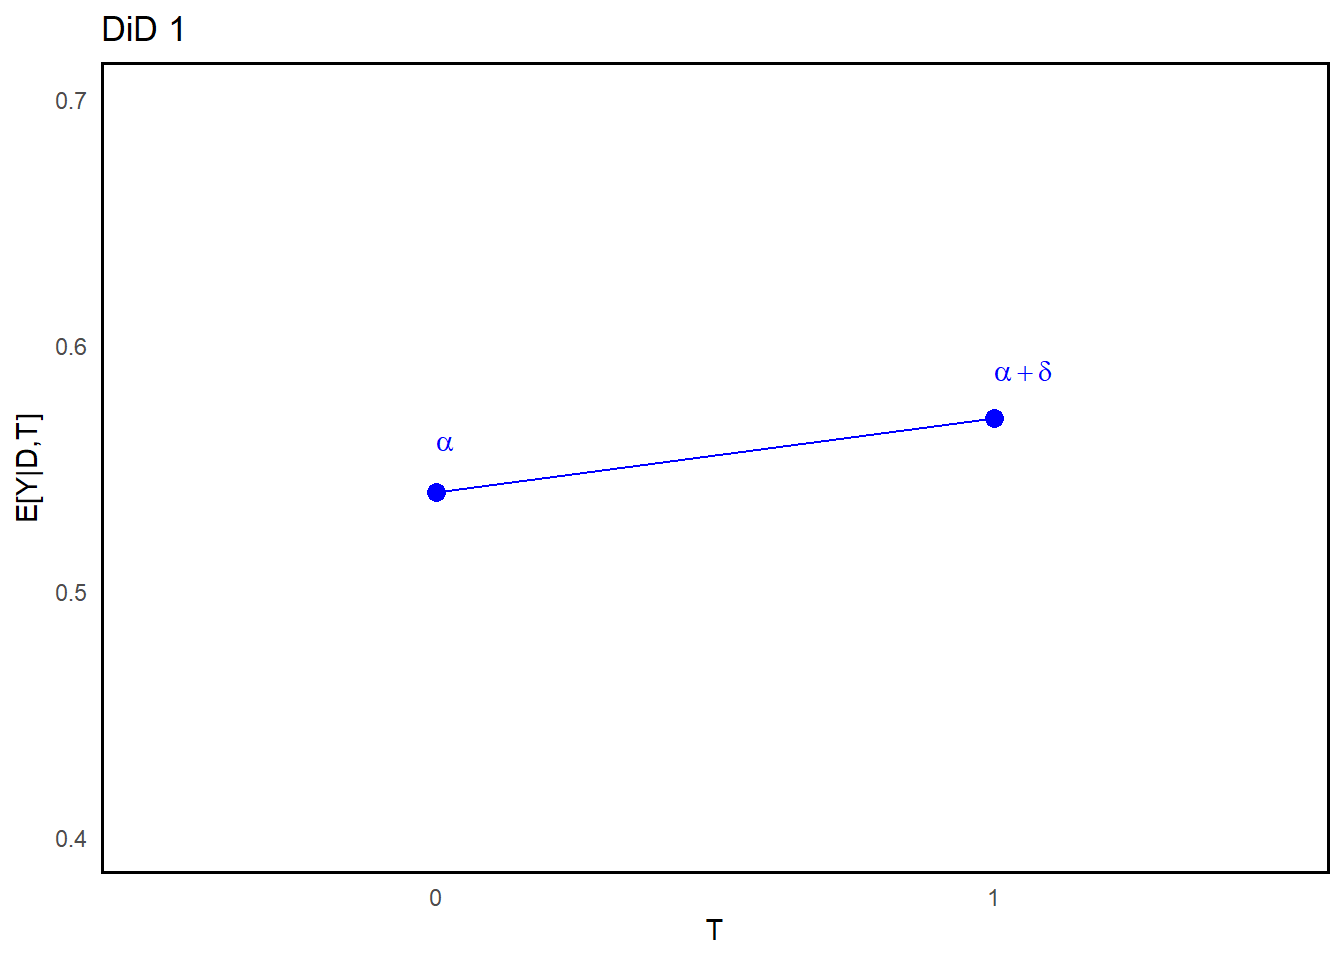
\includegraphics{paralleltrends_files/figure-pdf/fig-graph1-1.pdf}

  }

  \caption{\label{fig-graph1}Difference-in-Differences Plot 1}

  \end{figure}%

  \begin{figure}

  \centering{

  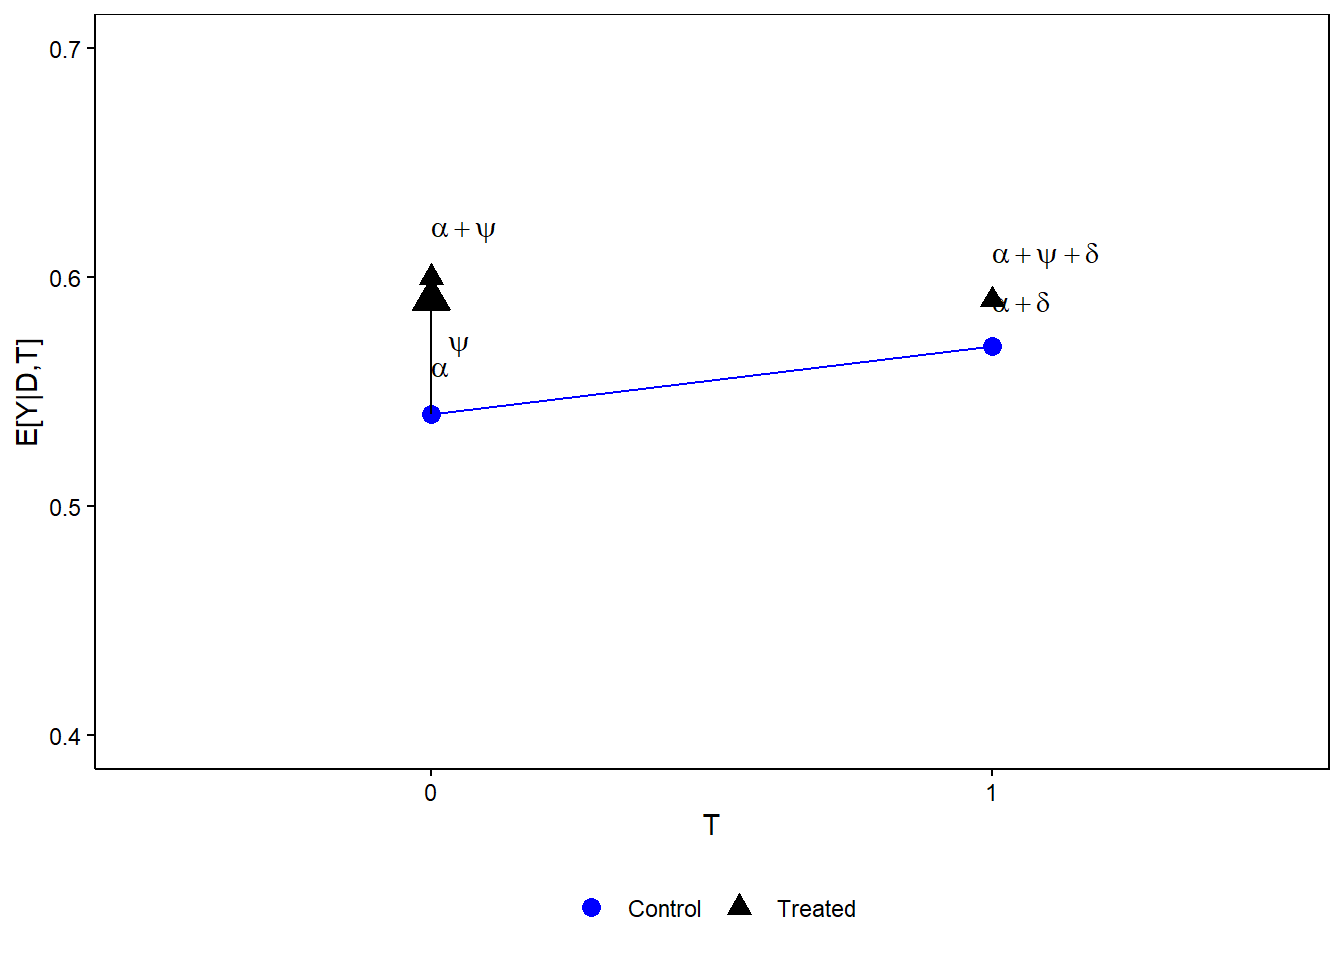
\includegraphics{paralleltrends_files/figure-pdf/fig-graph2-1.pdf}

  }

  \caption{\label{fig-graph2}Difference-in-Differences Plot 2}

  \end{figure}%

  \section{DiD and CIA}\label{did-and-cia}

  Do we need the CIA/Unconfoundedness assumption?\\
  \textbf{NO}, Why not?

  \begin{itemize}
  \item
    We do not identify the ATT as the coefficient on ( \(D_i\) ).
  \item
    With two sources of variation, both time and treatment group, we can
    identify the selection term in the pre-period,

    \[
    E[Y_i(0)|D_i=1,T_i=0] - E[Y_i(0)|D_i=0,T_i=0] = \psi
    \]
  \item
    Key assumption: selection doesn't change over time; i.e.,
    \emph{parallel/common trends}.
  \end{itemize}

  \section{Selection}\label{selection-1}

  Let us consider the first (cross-sectional) difference,

  \[
  \begin{aligned}
  &E[Y_{it}|D_i=1,T_t=1] - E[Y_{it}|D_i=0,T_t=1] \\
  &= E[Y_{it}(1)|D_i=1,T_t=1] - E[Y_{it}(0)|D_i=0,T_t=1] \\
  &= \underbrace{E[Y_{it}(1)|D_i=1,T_t=1] \textcolor{red}{- E[Y_{it}(0)|D_i=1,T_t=1]}}_{\text{ATT in period } t_0} \\
  &\quad \underbrace{\textcolor{red}{+ E[Y_{it}(0)|D_i=1,T_t=1]} - E[Y_{it}(0)|D_i=0,T_t=1]}_{\text{selection between groups}}
  \end{aligned}
  \]

  which is very similar to,

  \[
  E[Y_{it}(0)|D_i=1,T_t=0] - E[Y_{it}(0)|D_i=0,T_t=0]
  \]

  from the first period.

  With the parallel trends assumption,

  Selection is given by

  \[
  \underbrace{\textcolor{red}{E[Y_{it}(0)|D_i=1,T_t=1]}}_{\alpha + \psi + \delta} - \underbrace{E[Y_{it}(0)|D_i=0,T_t=1]}_{\alpha + \delta} = \psi
  \]

  and

  \[
  \underbrace{E[Y_{it}(0)|D_i=1,T_t=0]}_{\alpha + \psi} - \underbrace{E[Y_{it}(0)|D_i=0,T_t=0]}_{\alpha} = \psi
  \]

  \begin{itemize}
  \tightlist
  \item
    Permits level differences between treatment and control.
  \item
    Selection term is identified in pre-period.\footnote{Emphasizes
      importance of `no pre-emptive behaviour' assumption.}
  \end{itemize}

  \section{Difference-in-differences}\label{difference-in-differences}

  Again we can identify the ATT as a \emph{difference-in-differences},

  \[
  \begin{aligned}
  &\left[E[Y_{it}|D_i=1,T_t=1] - \textcolor{blue}{E[Y_{it}|D_i=0,T_t=1]}\right] \\
  &- \left[E[Y_{it}|D_i=1,T_t=0] - \textcolor{blue}{E[Y_{it}|D_i=0,T_t=0]}\right] \\
  &= \left[E[Y_{it}(1)|D_i=1,T_t=1] - \textcolor{blue}{E[Y_{it}(0)|D_i=0,T_t=1]}\right] \\
  &- \left[E[Y_{it}(0)|D_i=1,T_t=0] - \textcolor{blue}{E[Y_{it}(0)|D_i=0,T_t=0]}\right] \\
  &= \underbrace{\left[E[Y_{it}(1)|D_i=1,T_t=1] \textcolor{red}{- E[Y_{it}(0)|D_i=1,T_t=1]}\right]}_{\tau_{ATT}(t_0)} \\
  &+ \underbrace{\left[\textcolor{red}{E[Y_{it}(0)|D_i=1,T_t=1]} - \textcolor{blue}{E[Y_{it}(0)|D_i=0,T_t=1]}\right]}_{= \psi} \\
  &- \underbrace{\left[E[Y_{it}(0)|D_i=1,T_t=0] - \textcolor{blue}{E[Y_{it}(0)|D_i=0,T_t=0]}\right]}_{= \psi}
  \end{aligned}
  \]

  \begin{itemize}
  \tightlist
  \item
    Parallel trends allow us to pin down the selection component.
  \item
    We do not need unconfoundedness to rule out selection.
  \end{itemize}

  \section{DiD in Practice}\label{did-in-practice}

  \subsection{Multi-group-2-period}\label{multi-group-2-period}

  \textbf{In a `natural' experiment setting}, treatment is almost always
  assigned at a group-level setting: geographical, demographic, etc.

  Let (\(Y_{itc}\)) be the outcome of unit (\(i\)) in period ( \(t\)),
  member of assignment-group (\(c(i)\)),

  \[
  c(i) \in \{1, \ldots, c_0, c_0 + 1, \ldots, C\}
  \]

  where groups are:

  \begin{itemize}
  \tightlist
  \item
    Treated: ( \(1\), \(\ldots, c_0\) ) (no. treated groups = ( \(c_0\)
    ))
  \item
    Control: ( \(c_0 + 1, \ldots, C\) ) (no. control groups \(=\) (
    \(C - c_0\) ))
  \end{itemize}

  Thus,

  \[
  D_i = D_{c(i)} = \mathbf{1}\{c(i) \leq c_0\}
  \]

  \section{Group Assignment}\label{group-assignment}

  The relevant estimating equation is then,

  \[
  Y^{obs}_{itc} = \alpha + \psi D_{c} + \delta T_t + \beta D_{c} \cdot T_t + \varepsilon_{itc}
  \]

  \begin{itemize}
  \tightlist
  \item
    A model that can be estimated using repeated cross-sections or
    panel/longitudinal data.\footnote{This is also true for unit-level
      assignment, assuming sample selection of the subsequent
      cross-sections is independent of treatment.}
  \end{itemize}

  \section{Group Fixed Effects}\label{group-fixed-effects}

  Fixed effects notation is used extensively in Microeconometrics.

  Given a set of assignment-groups ( \(c = 1, 2, 3, \ldots, C\)),
  assignment-group FE's can be written as,

  \[
  \psi_c = \sum_{j=1}^{C} \psi_j \mathbf{1}\{c = j\}
  \]

  \begin{itemize}
  \tightlist
  \item
    A dummy variable for each value.
  \item
    Standard to drop the constant term in the regression equation.
  \item
    Implicitly, this is a group-specific constant.
  \end{itemize}

  \textbf{Parallel Trends Assumption (parametric version)}

  \[
  E[Y_{it}(0)|D_c,T_t] = \psi_c + \delta T_t
  \]

  Consider the two estimating equations,

  \[
  Y^{obs}_{itc} = \alpha + \psi D_c + \delta T_t + \beta_1 D_c \cdot T_t + \varepsilon_{itc}
  \]

  and

  \[
  Y^{obs}_{itc} = \psi_c + \delta T_t + \beta_2 D_c \cdot T_t + \epsilon_{itc}
  \]

  \begin{itemize}
  \tightlist
  \item
    (\hat{\beta}\_2 = \hat{\beta}\_1) \textbf{IF} group size does not
    change with time; i.e., a balanced panel of groups with stable group
    sizes. Group size need not be equal.
  \item
    Does not introduce bias.
  \item
    But, ( se(\hat{\beta}\_2) ) \textbf{tends to be} smaller than (
    se(\hat{\beta}\_1) )\footnote{`tends to be', because you also
      decrease the degree of freedom.}.
  \end{itemize}

  With group FE's we \emph{typically} explain more of the variation in (
  Y(0) ).

  \section{Example: UK Policy}\label{example-uk-policy}

  Suppose Scotland and Wales introduce a policy to restrict access to
  fast food in year (\(t_0\)) and you have individual-level measures of
  BMI from across the UK.

  \begin{itemize}
  \item
    (\$D\_c = \mathbf{1}{c \leq 2}\$)
  \item
    Estimating equations,

    \[
    Y^{obs}_{itc} = \alpha + \psi D_c + \delta T_t + \beta_1 D_c \cdot T_t + \varepsilon_{itc}
    \]

    and

    \[
    Y^{obs}_{itc} = \underbrace{\sum_{j=1}^{4} \psi_j \mathbf{1}\{c = j\}}_{\psi_c} + \delta T_t + \beta_2 D_c \cdot T_t + \epsilon_{itc}
    \]
  \end{itemize}

  \section{Unit Fixed Effects}\label{unit-fixed-effects}

  Suppose, you have \textbf{panel/longitudinal data}, then the
  specification,

  \[
  Y^{obs}_{itc} = \alpha_i + \delta T_t + \beta_3 D_c\cdot T_t + \upsilon_{itc}
  \]

  will \textbf{typically} yield an even more efficient estimator.

  \begin{itemize}
  \tightlist
  \item
    \(\hat{\beta}_3=\hat{\beta}_2=\hat{\beta}_1\) \textbf{IF} all units
    are observed in all periods; i.e., a balanced panel of units.
  \item
    Does not introduce bias.
  \item
    \(se(\hat{\beta}_3)\) \textbf{tends to be} smaller than
    \(se(\hat{\beta}_2)\), which \emph{tends to be} smaller than
    \(se(\hat{\beta}_1)\).
  \item
    Increases the power of the test for \(H_0: \tau_{ATT}=0\).
  \item
    Higher dimensions of FEs \emph{tend to} yield lower variance
    estimators.
  \end{itemize}

  \section{Adding Covariates}\label{adding-covariates-2}

  There are two reasons to add \textbf{GOOD} covariates to the model:

  \begin{enumerate}
  \def\labelenumii{\arabic{enumii}.}
  \tightlist
  \item
    Improve the precision of estimates and increase power.
  \item
    For identification (when \emph{unconditional} parallel trends fail).
  \end{enumerate}

  \textbf{Conditional Parallel Trends Assumption (General version)}

  \[
  \begin{aligned}
  &E[Y_{it}(0)|D_i=0,T_t=1,X_i'] - E[Y_{it}(0)|D_i=0,T_t=0,X_i'] \\
  &= E[Y_{it}(0)|D_i=1,T_t=1,X_i'] - E[Y_{it}(0)|D_i=1,T_t=0,X_i']
  \end{aligned}
  \]

  or

  \textbf{Conditional Parallel Trends Assumption (CEF version)}

  \[
  E[Y_{it}(0)|D_i,T_t,X_{it}] = \alpha + \psi D_i + \delta T_t + X_{it}'\gamma
  \]

  \begin{itemize}
  \tightlist
  \item
    A \emph{weaker} assumption.
  \item
    In a balanced panel, time-invariant differences across groups are
    captured by treatment-group dummy (or assignment-group/unit FEs).
  \end{itemize}

  \textbf{Warning:} \textgreater{} If estimates are sensitive to the
  inclusion of good covariates, it suggests that one of the identifying
  assumptions \emph{may} have failed. \textbf{Why is the covariate
  composition of the groups changes differentially over time?} Could be
  due to non-parallel trends or switching between groups.

  With \emph{only 2 periods} of data, there is no test of the parallel
  trends assumption.

  \begin{itemize}
  \tightlist
  \item
    Intuitively, similar groups \emph{may} be more likely to follow
    parallel trends.
  \item
    Argument for matching on covariates in pre-period. For example,
    PSM-DID.
  \end{itemize}

  \section{DiD in Practice - Multiple Time
  Periods}\label{did-in-practice---multiple-time-periods}

  Suppose you had more than 2 periods of data, you might then choose to
  add time-fixed effects,

  \[
  Y^{obs}_{itc} = \psi_c + \delta_t + \beta_3 D_c\cdot T_t + \upsilon_{itc}
  \]

  where \(T_t=\mathbf{1}\{t\geq t_0\}\) and \(t_0\) is the period of
  treatment.

  \begin{itemize}
  \tightlist
  \item
    However, we first need to discuss \emph{dynamic} treatment effects.
  \end{itemize}

  \textbf{Next lecture.}

  \section{Card \& Krueger (1994)}\label{card-krueger-1994}

  This paper\footnote{Angrist \& Pischke attribute the first use of DiD
    in Economics to Obenauer \& von den Nienburg (1915) (see page 228 of
    \emph{Mostly Harmless Econometrics}).},

  \begin{itemize}
  \item
    arguably, established difference-in-difference as the central tool
    in Applied Microeconomics research;
  \item
    turned the literature on the minimum wage upside down;
  \item
    won David Card the Nobel Prize in Economics;
  \item
    and started the closest thing to a fight in academic
    Economics.\footnote{The debate between Card and Krueger (since
      deceased, 2019), and Neumark and Wascher is ongoing.}
  \end{itemize}

  \subsection{Pre-1990's Literature}\label{pre-1990s-literature}

  \begin{itemize}
  \tightlist
  \item
    Most of the literature supported the idea that higher minimum wages
    reduce employment.
  \item
    Wellington (1991) \& Brown et al.~(1983): A 10\% increase in minimum
    wage reduces teen employment by 1\%.
  \item
    Largely based on time-series evidence (Brown et al., 1982) or
    cross-country studies.
  \end{itemize}

  \begin{quote}
  ``Isolating the impacts of labor market institutions is inherently
  difficult\ldots{} Identification issues essentially result from the
  endogeneity of labor market institutions and the interactions between
  them\ldots{} makes it difficult to attribute variations in outcomes to
  the institutions themselves, rather than other features of the
  societies in which they exist.'' - Baetcherman (2012)
  \end{quote}

  \textbf{Card \& Krueger (AER, 1994)} is a seminal paper in this
  literature\footnote{And Katz \& Krueger (ILR Review, 1992)},

  \begin{itemize}
  \tightlist
  \item
    Increase in New Jersey minimum wage from \$4.25 to \$5.05, April
    1992.
  \item
    Examine the impact on employment at fast food outlets (low wage
    jobs).
  \item
    Use Pennsylvania as a control group in a \textbf{DiD research
    design}.
  \item
    Find \textbf{no evidence} of a negative employment effect.
  \end{itemize}

  This paper highlights the fact that you can make strong conclusions
  from what is effectively a very simple research design.

  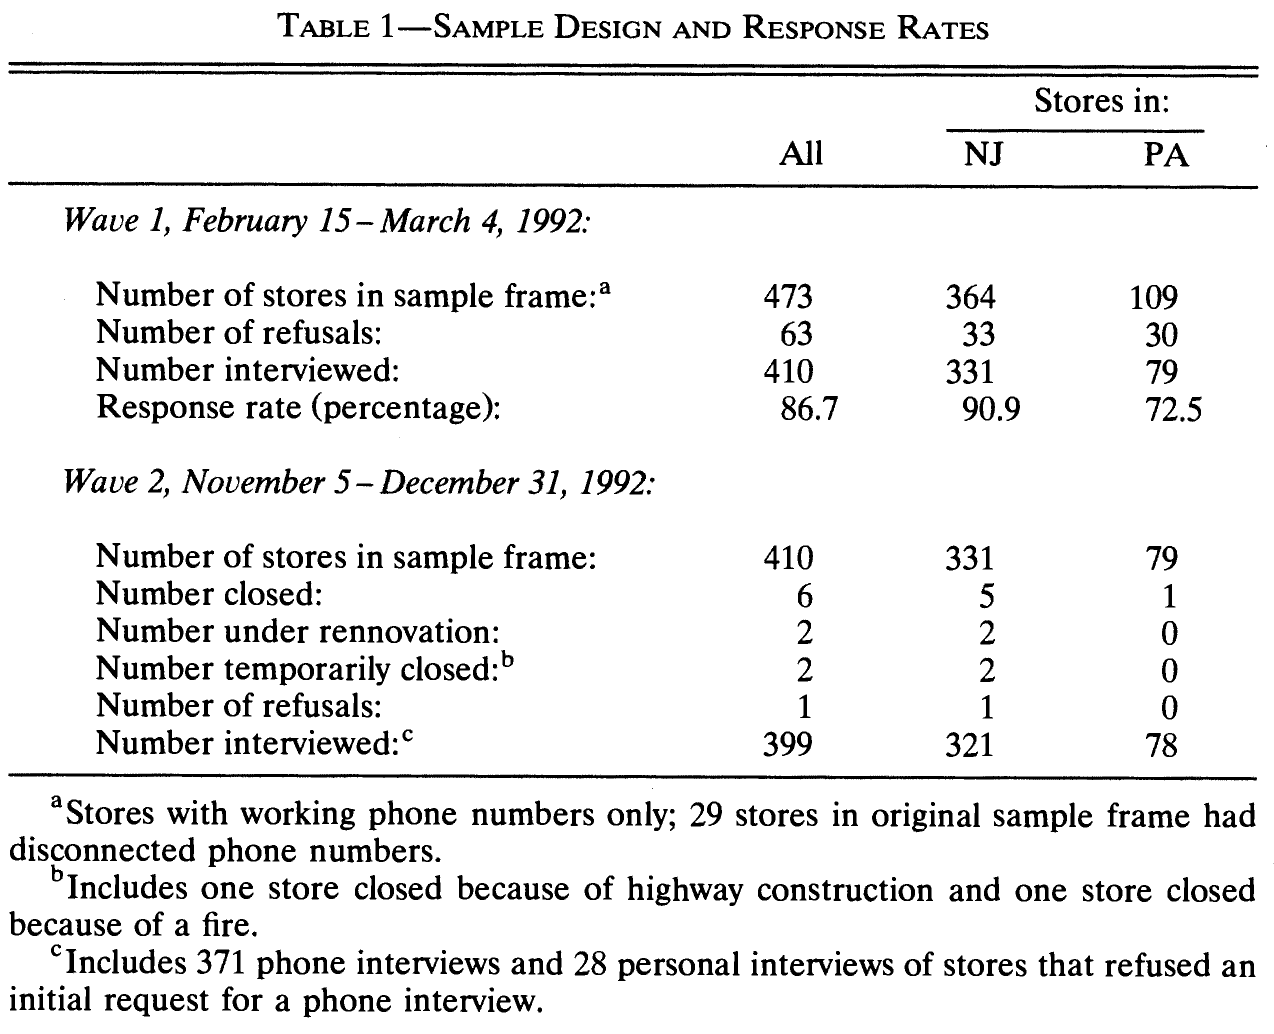
\includegraphics{docs/images/diff-card-krueger-1994-tab1.png}

  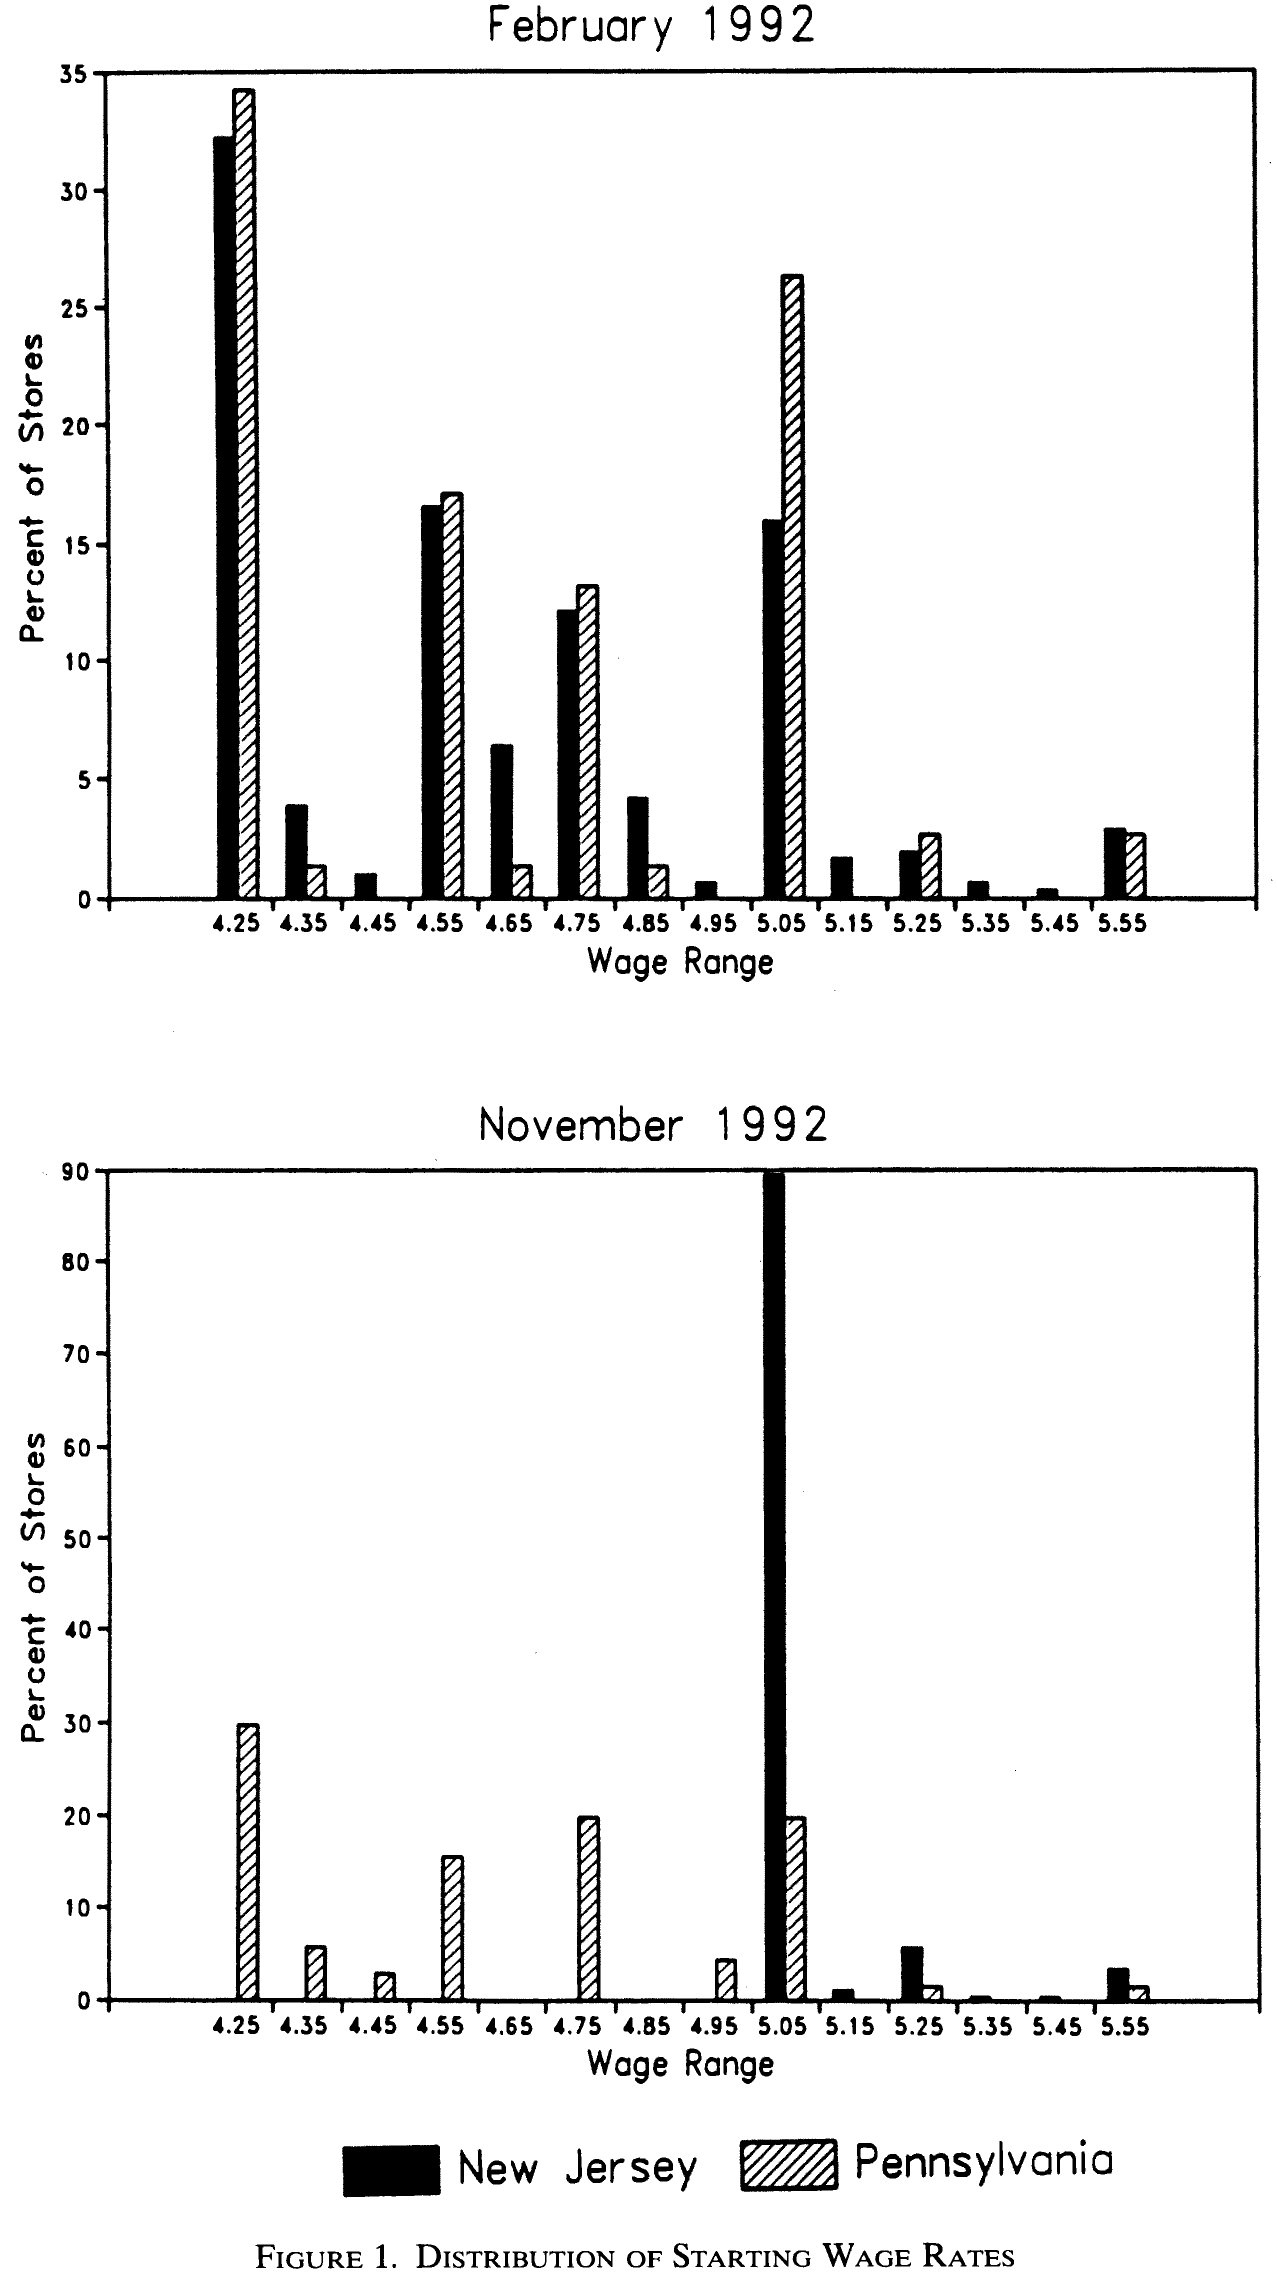
\includegraphics{docs/images/diff-card-krueger-1994-fig1.png}

  \section{Legislative Change}\label{legislative-change}

  This minimum wage change \textbf{was not unexpected}:

  \begin{itemize}
  \tightlist
  \item
    Federal minimum wage is the floor to all state level minimum wages.
  \item
    Federal increase from \$3.35 to \$3.80 in April 1990.
  \item
    Federal increase from \$3.80 to \$4.25 in April 1991.
  \item
    New Jersey chose to increase its own minimum wage to \$5.05
    effective April 1992, giving it the highest minimum wage in the
    country.
  \item
    Opposed by business leaders, but the opposition lost an appeal
    (March, 1992) by a close margin.
  \end{itemize}

  This last-minute appeal and close election do create some uncertainty.

  \section{Research Design}\label{research-design}

  Card \& Krueger (1994) implement a basic difference-in-difference
  research design

  \[
  \tau_{ATT} = \big(E[Y_{it}|T_t=1,D_i=1] - E[Y_{it}|T_t=0,D_i=1]\big) - \big(E[Y_{it}|T_t=1,D_i=0] - E[Y_{it}|T_t=0,D_i=0]\big)
  \]

  where \(T_t = \mathbf{1}{\text{after April 1992}}\), and

  \[
  D_i = 
  \begin{cases}
  1 & \text{New Jersey} \\
  0 & \text{Pennsylvania}
  \end{cases}
  \]

  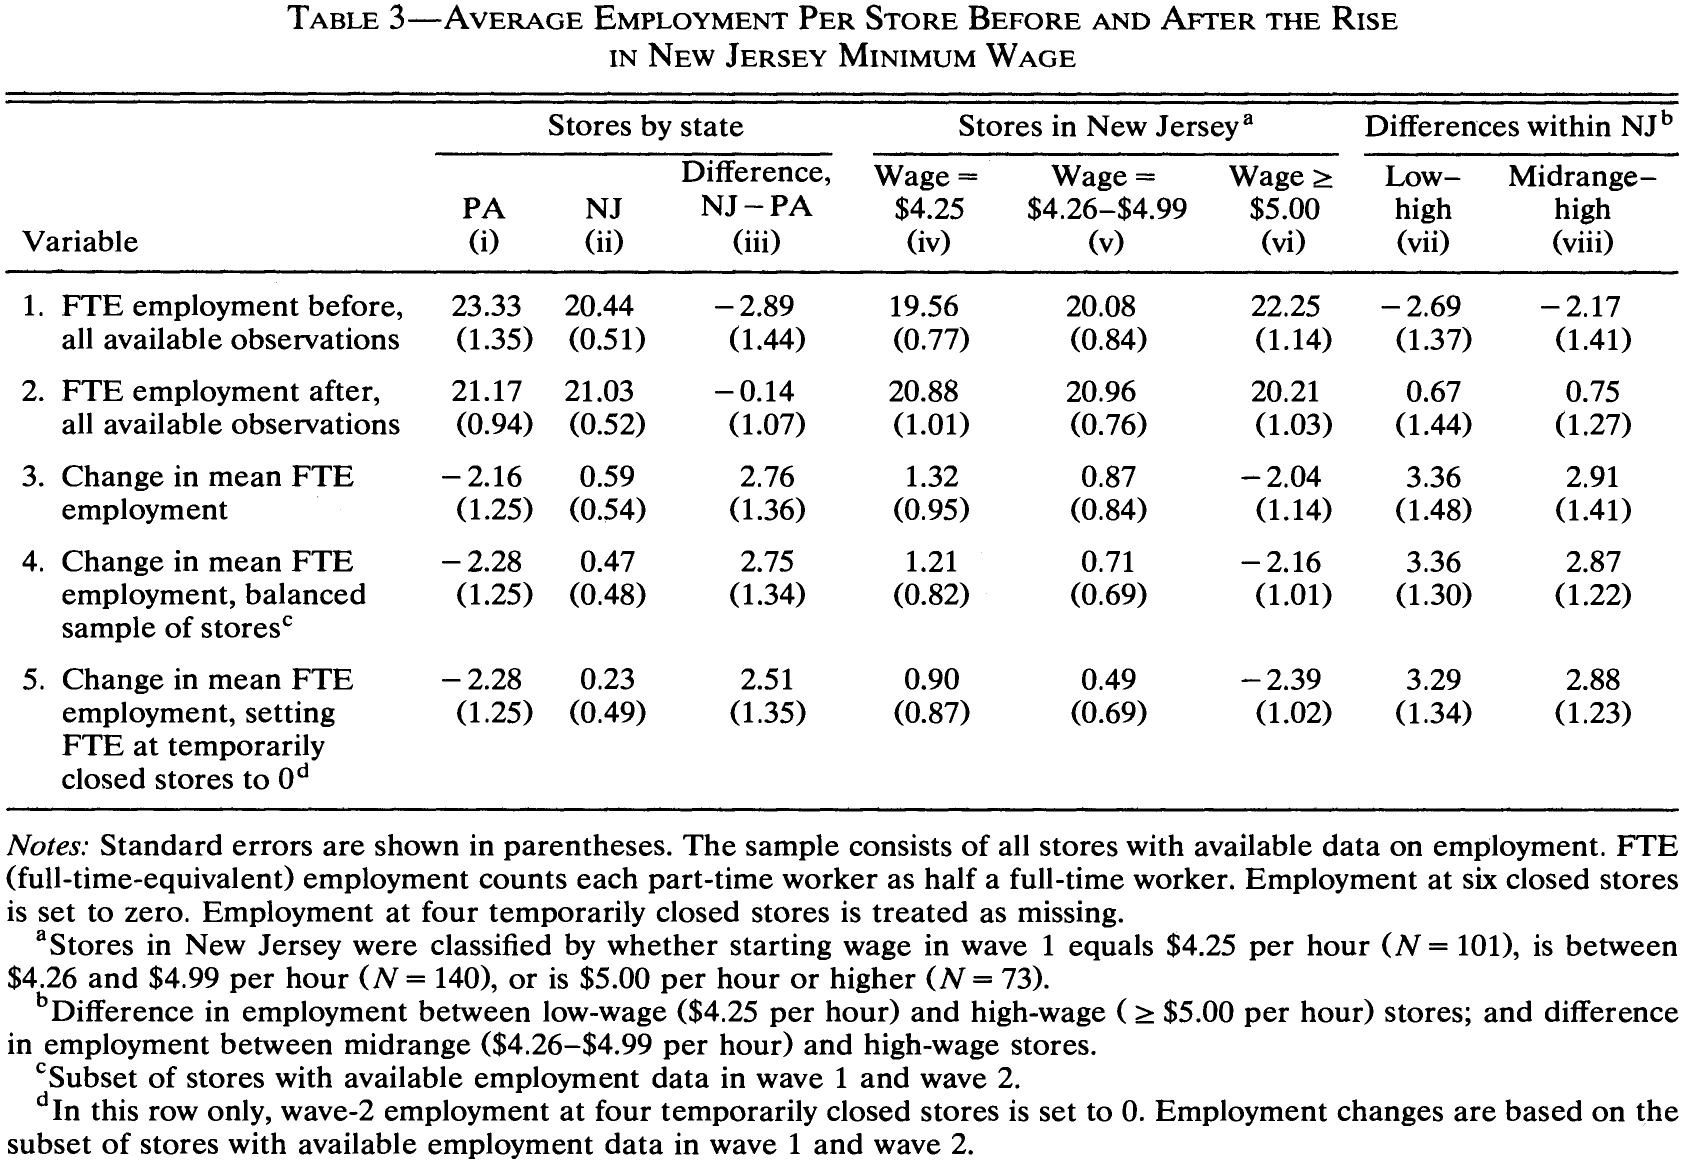
\includegraphics{docs/images/diff-card-krueger-1994-tab3.png}\\
  \strut \\
  Conclusion,

  \begin{itemize}
  \tightlist
  \item
    No evidence of a negative effect, as competitive models would
    predict.
  \item
    If anything, some evidence of a small positive effect, as suggested
    by monopsonistic models.
  \item
    Card \& Krueger (1994) don't show pre-trends to help persuade you
    that the parallel trends assumption is likely to hold.
  \item
    After this paper comes the rebuttal by Neumark \& Wascher (2000,
    AER), followed immediately by a response from Card \& Krueger (2000,
    AER).
  \item
    This is just round 1 of what is a multi-round debate. The discussion
    has now shifted away from state-level minimum wages to the study of
    city-specific policies.
  \end{itemize}

  \chapter{Dynamic Treatment Effects}\label{dynamic-treatment-effects}

  \section{Set-up}\label{set-up}

  Today's discussion will concern,

  Once treatment is applied it remains fixed.

  \begin{itemize}
  \tightlist
  \item
    If treatment is temporary, the model will capture long-term effects.
  \end{itemize}

  \section{Dynamic TE's}\label{dynamic-tes}

  Suppose that the treatment effect is indeed dynamic:

  \begin{tcolorbox}[enhanced jigsaw, bottomrule=.15mm, coltitle=black, arc=.35mm, left=2mm, opacityback=0, leftrule=.75mm, colbacktitle=quarto-callout-note-color!10!white, title={Note}, toprule=.15mm, bottomtitle=1mm, breakable, colframe=quarto-callout-note-color-frame, opacitybacktitle=0.6, titlerule=0mm, colback=white, rightrule=.15mm, toptitle=1mm]

  For all ( \(t=0,1,2,...,T\))

  \[
  Y_{it}(1)-Y_{it}(0) = \tau_{it}
  \]

  \end{tcolorbox}

  It helps to normalize time to \textbf{event-time},

  \[
  s=t-S_{i}
  \]

  where (\(S_i\)) is the time period in which unit (\(i\)) first
  receives the treatment.

  \begin{itemize}
  \tightlist
  \item
    (\(S_i\)) could be determined at the assignment-group level,
  \end{itemize}

  \[
  S_i=S_c
  \]

  Given time periods (\(t=0,1,...T\)), ( \(s=-T,..,-1,0,1,...,T\)). The
  dynamic treatment effect is specified as,

  \begin{tcolorbox}[enhanced jigsaw, bottomrule=.15mm, coltitle=black, arc=.35mm, left=2mm, opacityback=0, leftrule=.75mm, colbacktitle=quarto-callout-note-color!10!white, title={Note}, toprule=.15mm, bottomtitle=1mm, breakable, colframe=quarto-callout-note-color-frame, opacitybacktitle=0.6, titlerule=0mm, colback=white, rightrule=.15mm, toptitle=1mm]

  \[
  Y_{its}(1)-Y_{its}(0) = \tau_{is}
  \]

  \end{tcolorbox}

  \begin{itemize}
  \tightlist
  \item
    The relevant unit of time is event-time, not calendar
    time.\footnote{This rules out dynamic TEs which change over
      (calendar) time.}
  \item
    In a 2-group-multiple-period setting ( \(s\) ) does not vary
    independently of ( \(t\) ) for the treated units.
  \item
    This set-up becomes more useful when describing multi-cohort
    settings.
  \end{itemize}

  \section{Dynamic TE's}\label{dynamic-tes-1}

  \begin{tcolorbox}[enhanced jigsaw, bottomrule=.15mm, coltitle=black, arc=.35mm, left=2mm, opacityback=0, leftrule=.75mm, colbacktitle=quarto-callout-note-color!10!white, title={Note}, toprule=.15mm, bottomtitle=1mm, breakable, colframe=quarto-callout-note-color-frame, opacitybacktitle=0.6, titlerule=0mm, colback=white, rightrule=.15mm, toptitle=1mm]

  \textbf{Treatment Cohort}\\
  A group of individuals treated at the same time, ( \$S\_i\$).

  \end{tcolorbox}

  \begin{itemize}
  \tightlist
  \item
    In a staggered-DiD model or event-study, there are multiple cohorts.
  \item
    For \emph{never treated} groups, \[
    S_i = \infty
    \]
  \item
    A never treated and not-yet/future treated group are NOT the same.
  \end{itemize}

  \section{2-group-2-period}\label{group-2-period}

  Recall from lecture 4.1,

  \[
  Y^{obs}_{it} = \alpha + \psi D_i + \delta T_t + \beta D_i \cdot T_t + \varepsilon_{it}
  \]

  Using this new notation, we can rewrite this equation as,

  \[
  Y^{obs}_{it} = \psi D_i + \delta_t + \beta \mathbf{1}\{s \geq 0\} + \varepsilon_{it}
  \]

  \begin{itemize}
  \tightlist
  \item
    Time FEs are the same as a post-treatment dummy with 2 periods.
  \item
    For the treated group, ( \(S_i = t_0\) ).
  \item
    For the control group, ( \$S\_i = \infty \$ ).
  \item
    (
    \(D_i \cdot T_t = \mathbf{1}{t \geq S_i} = \mathbf{1}{s \geq 0}\));
    which implies, \[
    \Rightarrow \mathbf{1}\{s = t - \infty \geq 0\} = 0 \quad \text{**always.**}
    \]
  \end{itemize}

  \section{Multi-group-2-period}\label{multi-group-2-period-1}

  Recall from lecture 4.1,

  \[
  Y^{obs}_{itc} = \psi_c + \delta T_t + \beta D_c \cdot T_t + \varepsilon_{itc}
  \]

  Using this new notation, we can rewrite this equation as,

  \[
  Y^{obs}_{itc} = \psi_c + \delta_t + \beta \mathbf{1}\{s \geq 0\} + \varepsilon_{itc}
  \]

  \begin{itemize}
  \tightlist
  \item
    For the treated groups (( \(c \leq c_0\) )), ( \(S_c = t_0\) ).
  \item
    For the control groups (( \(c > c_0\))), ( \$S\_c = \infty\$ ).
  \item
    ( \(D_c \cdot T_t = \mathbf{1}{t \geq S_c} = \mathbf{1}{s \geq 0}\)
    )
  \item
    In both these applications, there is a one-to-one mapping from event
    to calendar time.
  \end{itemize}

  \chapter{Multi-Period DiD}\label{multi-period-did}

  We can define a more flexible version of the parallel
  trends,\footnote{For example, see discussion on Eissa \& Liebman
    (1996).}

  \begin{tcolorbox}[enhanced jigsaw, bottomrule=.15mm, coltitle=black, arc=.35mm, left=2mm, opacityback=0, leftrule=.75mm, colbacktitle=quarto-callout-note-color!10!white, title={Note}, toprule=.15mm, bottomtitle=1mm, breakable, colframe=quarto-callout-note-color-frame, opacitybacktitle=0.6, titlerule=0mm, colback=white, rightrule=.15mm, toptitle=1mm]

  \textbf{Parallel Trends Assumption (Parametric version)}\\
  \[
  E[Y_{it}(0)|D_i, t] = \psi D_i + \delta_t
  \]

  \end{tcolorbox}

  or,

  \begin{tcolorbox}[enhanced jigsaw, bottomrule=.15mm, coltitle=black, arc=.35mm, left=2mm, opacityback=0, leftrule=.75mm, colbacktitle=quarto-callout-note-color!10!white, title={Note}, toprule=.15mm, bottomtitle=1mm, breakable, colframe=quarto-callout-note-color-frame, opacitybacktitle=0.6, titlerule=0mm, colback=white, rightrule=.15mm, toptitle=1mm]

  \textbf{Parallel Trends Assumption (Parametric version)}\\
  \[
  E[Y_{itc}(0)|c, t] = \psi_c + \delta_t
  \] with group FEs.

  \end{tcolorbox}

  \begin{tcolorbox}[enhanced jigsaw, bottomrule=.15mm, coltitle=black, arc=.35mm, left=2mm, opacityback=0, leftrule=.75mm, colbacktitle=quarto-callout-note-color!10!white, title={Note}, toprule=.15mm, bottomtitle=1mm, breakable, colframe=quarto-callout-note-color-frame, opacitybacktitle=0.6, titlerule=0mm, colback=white, rightrule=.15mm, toptitle=1mm]

  \textbf{Parallel Trends Assumption (Parametric version)}\\
  \[
  E[Y_{it}(0)|D_i, t] = \alpha_i + \delta_t
  \] with unit FEs.

  \end{tcolorbox}

  \section{Multi-Period DiD}\label{multi-period-did-1}

  However, if we specify the model as,

  \[
  Y^{obs}_{it} = \psi D_i + \delta_t + \beta \mathbf{1}\{s \geq 0\} + \upsilon_{it}
  \]

  where (\(\beta\)) captures the ATT in all post-treatment periods, then
  we have proposed a linear regression model that best characterizes,

  \begin{tcolorbox}[enhanced jigsaw, bottomrule=.15mm, coltitle=black, arc=.35mm, left=2mm, opacityback=0, leftrule=.75mm, colbacktitle=quarto-callout-note-color!10!white, title={Note}, toprule=.15mm, bottomtitle=1mm, breakable, colframe=quarto-callout-note-color-frame, opacitybacktitle=0.6, titlerule=0mm, colback=white, rightrule=.15mm, toptitle=1mm]

  \textbf{Static Treatment Effects}

  \[
  Y_{it}(1) - Y_{it}(0) = \tau_{i}
  \]

  \end{tcolorbox}

  \[
  \tau_{ATT}(s) = E[Y_{it}(1) - Y_{it}(0)|D_i = 1, t = S_i + s] = \tau_{ATT} \quad \forall \; s \geq 0
  \]

  \section{Dynamic DiD}\label{dynamic-did}

  If TEs are dynamic, it is better to estimate either,

  \begin{enumerate}
  \def\labelenumii{\arabic{enumii}.}
  \tightlist
  \item
    Semi-dynamic model,
  \end{enumerate}

  \[
  Y^{obs}_{it} = \psi D_i + \delta_t + \sum_{j \geq 0} \beta_j \mathbf{1}\{s = j\} + \upsilon_{it}
  \]

  \begin{enumerate}
  \def\labelenumii{\arabic{enumii}.}
  \setcounter{enumii}{1}
  \tightlist
  \item
    Dynamic model,
  \end{enumerate}

  \[
  Y^{obs}_{it} = \psi D_i + \delta_t + \sum_{j \neq -1} \beta_j \mathbf{1}\{s = j\} + \upsilon_{it}
  \]

  \begin{itemize}
  \tightlist
  \item
    In applied settings, you should always specify such a model with
    time FEs, and not a single post-treatment dummy. Failure to do so
    will typically lead to a false counterfactual.\footnote{Can you
      demonstrate this?}
  \item
    You have to normalize 1 period. It does not have to be ( s = -1 ),
    but should be a pre-period.
  \end{itemize}

  \section{Dynamic DiD (Continued)}\label{dynamic-did-continued}

  Consider the dynamic specification,

  \[
  Y^{obs}_{it} = \psi D_i + \delta_t + \sum_{j \neq -1} \beta_j \mathbf{1}\{s = j\} + \upsilon_{it}
  \]

  \begin{itemize}
  \tightlist
  \item
    We must exclude at least one of the event-time dummies. Standard to
    exclude pre-treatment period.
  \end{itemize}

  \textbf{QUESTION:} Assuming parallel trends and all necessary
  exclusion restrictions, how would we define ( \(\beta_2\) )?

  Proof:

  Single period of treatment: \(t_0\)

  Control group \(S_i = \infty\)

  \(\beta_2\) event-time \(s = 2\).

  \[
  1 \{S = 2\} = D_i \cdot 1 \{t = t_0+2\}.
  \]

  \[
  \beta_1 = 
  \left[ E[Y_t | D_i=1, t=t_0+2] - E[Y_t | D_i=0, t=t_0+2] \right] - 
  \left[ E[Y_t | D_i=1, t=t_0-1] - E[Y_t | D_i=0, t=t_0-1] \right]
  \]

  \[
  = E[Y_t(1) - Y_t(0) | D_i=1, t=t_0+2] 
  \]

  \[
  + \textcolor{red}{E[Y_t(0) | D_i=1, t=t_0+2] - E[Y_t(0) | D_i=0, t=t_0+2]}
  \]

  \[
  - \textcolor{red}{E[Y_t(1) | D_i=1, t=t_0-1] - E[Y_t(0) | D_i=0, t=t_0-1]}
  \]

  Where \(\textcolor{red}{\phi + \delta_{t2}}\) and
  \(\textcolor{red}{\delta_{t-1}}\) are the effects to be controlled
  for.

  \section{Dynamic DiD (Exclusion
  Restrictions)}\label{dynamic-did-exclusion-restrictions}

  Notice: - Linear model can identify treatment effects up to a
  normalized period. - We must assume,

  \begin{tcolorbox}[enhanced jigsaw, bottomrule=.15mm, coltitle=black, arc=.35mm, left=2mm, opacityback=0, leftrule=.75mm, colbacktitle=quarto-callout-note-color!10!white, title={Note}, toprule=.15mm, bottomtitle=1mm, breakable, colframe=quarto-callout-note-color-frame, opacitybacktitle=0.6, titlerule=0mm, colback=white, rightrule=.15mm, toptitle=1mm]

  \textbf{Exclusion restriction: No pre-emptive behaviour}

  \[
  E[Y_{it}|D_i = 1, t = t_0 + j] = E[Y_{it}(0)|D_i = 1, t = t_0 + j]
  \]

  for \textbf{some} (\(j \< 0\)).

  \end{tcolorbox}

  \begin{itemize}
  \tightlist
  \item
    Pre-emptive behaviour biases both pre-treatment \textbf{and
    post-treatment} TE estimates.
  \end{itemize}

  \section{Test parallel trends}\label{test-parallel-trends}

  \textbf{Assuming no pre-emptive behaviour}, the test,

  \[
  H_0: \beta_s = 0 \quad \forall \quad s < 0
  \]

  is a valid test for parallel trends \textbf{in the pre-treatment
  period}.

  \[
  \begin{aligned}
  \beta_s = & \left[\underbrace{E[Y_{it}|D_i = 1, t = t_0 + s] - E[Y_{it}|D_i = 1, t = t_0 - 1]}_{\text{Pre-trend of treated.}}\right] \\
  & - \left[\underbrace{\textcolor{blue}{E[Y_{it}|D_i = 0, t = t_0 + s] - E[Y_{it}|D_i = 0, t = t_0 - 1]}}_{\text{Pre-trend of control.}}\right]
  \end{aligned}
  \]

  for (\(s \< 0\)) and (\(s \neq -1\)).\footnote{Here, (\(s=-1\)) is the
    normalized period.}

  \section{Dynamic DiD (Visualization)}\label{dynamic-did-visualization}

  The problem can be how to distinguish between, - a failure of parallel
  trends, - and pre-emptive behaviour.

  {[}Alternative DID Plot{]}

  \section{Dynamic DiD
  (Renormalization)}\label{dynamic-did-renormalization}

  If there appears to be pre-emptive behaviour - and a reason for its
  presence - you can always renormalize the excluded base period.

  Here goes the other figure (I do not have it yet)

  include another graph here

  \section{Next-up}\label{next-up-2}

  \begin{itemize}
  \tightlist
  \item
    `Things Fall Apart' - The problems with dynamic/staggered DiD and
    two-way FEs
  \item
    What to do.
  \item
    Generalized two-way FEs models
  \item
    Synthetic Control
  \end{itemize}

  \section{\texorpdfstring{Example:
  \href{https://www.nber.org/papers/w5158}{Eissa \& Liebman
  (1996)}}{Example: Eissa \& Liebman (1996)}}\label{example-eissa-liebman-1996}

  \textbf{Example: Eissa \& Liebman (1996)}

  \section{Set-up: EITC}\label{set-up-eitc}

  Countries create tax credits for a number of reasons, these are
  typically after tax reimbursements based eligibility in certain
  criteria. Many are simply used to transfer income to a targeted
  population, and do not (intentionally) induce any behavioural
  response.

  \begin{itemize}
  \tightlist
  \item
    However, the \textbf{Earned} Income Tax Credit (EITC) is a uniquely
    targeted public policy that aims to both assist poorer, more
    vulnerable households while also incentivizing labour force
    participation (Holz \& Scholz, 2003).
  \end{itemize}

  The EITC aims to solve the following problem:

  \begin{tcolorbox}[enhanced jigsaw, bottomrule=.15mm, coltitle=black, arc=.35mm, left=2mm, opacityback=0, leftrule=.75mm, colbacktitle=quarto-callout-note-color!10!white, title={Note}, toprule=.15mm, bottomtitle=1mm, breakable, colframe=quarto-callout-note-color-frame, opacitybacktitle=0.6, titlerule=0mm, colback=white, rightrule=.15mm, toptitle=1mm]

  How do you redistribute money to poorer households without inducing a
  negative income effect? And can you design a policy that actually
  increases labour force participation while redistributing income.

  \end{tcolorbox}

  The tax credit increases in value with your earned income up to a
  threshold\ldots{}

  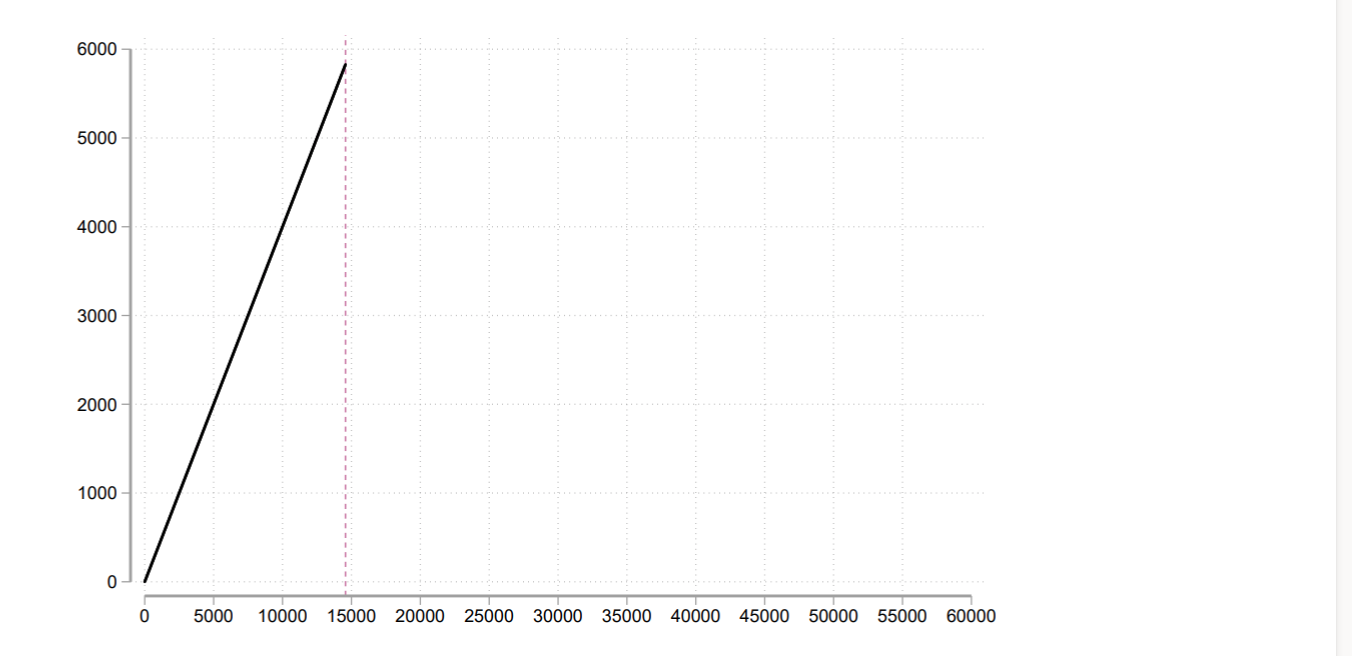
\includegraphics{docs/images/EL1.png}

  \textbf{Figure}: The tax credit is 40\% of earned income for the first
  \$14570
  (\href{https://www.cbpp.org/research/policy-basics-the-earned-income-tax-credit}{2019
  parameters} based on single earner with two children)

  \ldots at which point it is flat up to a second threshold\ldots{}

  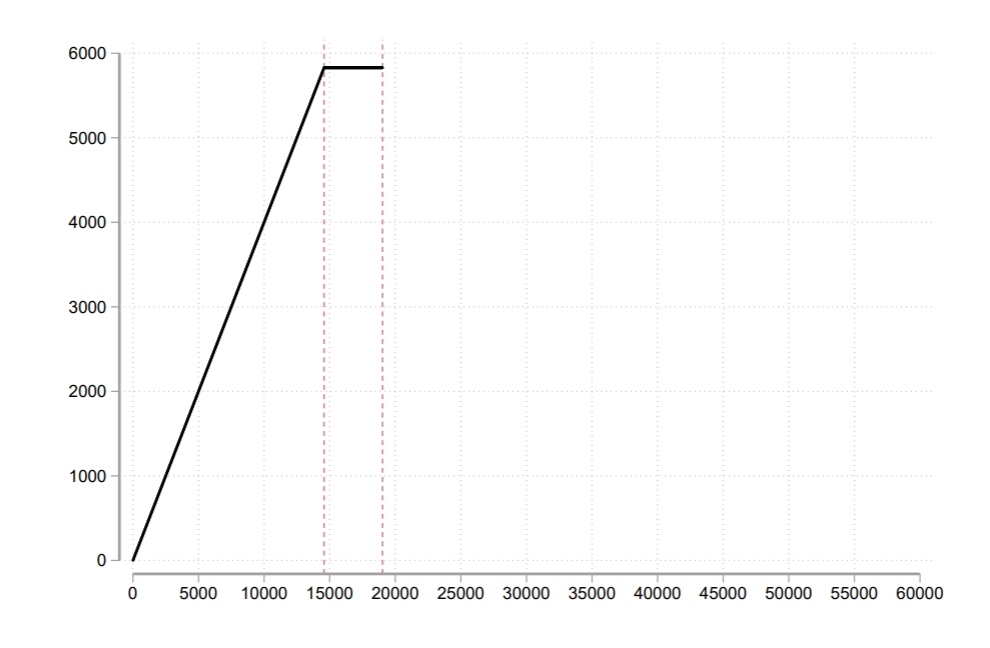
\includegraphics{docs/images/EL2.png}

  \textbf{Figure}: The maximum is \$5828
  (\href{https://www.cbpp.org/research/policy-basics-the-earned-income-tax-credit}{2019
  parameters} based on single earner with two children)

  \ldots{} and then is fazed out
\end{enumerate}

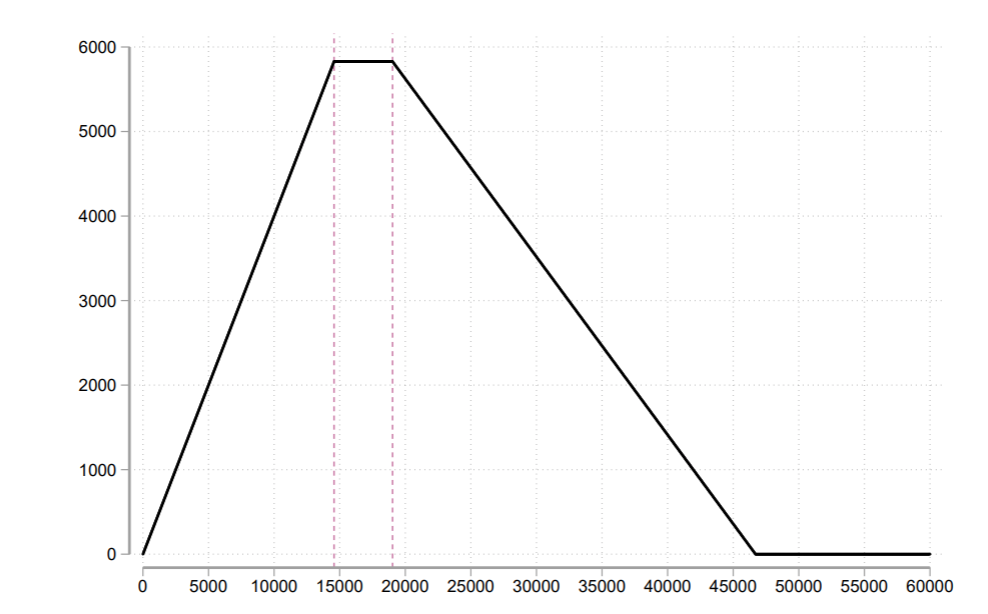
\includegraphics{docs/images/EL3.png}

\textbf{Figure}: The phase out rate is 21.06\% which ends at \$46703
(\href{https://www.cbpp.org/research/policy-basics-the-earned-income-tax-credit}{2019
parameters} based on single earner with two children)

Set up:

\begin{enumerate}
\def\labelenumi{\arabic{enumi}.}
\item
  PHASE IN: acts as a subsidy to work: incentive to earn more
\item
  PLATEAU: no subsidy, and hence no additional incentive to work more
\item
  PHASE OUT: effectively a tax on every additional dollar earned:
  disincentive to earn more
\end{enumerate}

\begin{tcolorbox}[enhanced jigsaw, bottomrule=.15mm, coltitle=black, arc=.35mm, left=2mm, opacityback=0, leftrule=.75mm, colbacktitle=quarto-callout-note-color!10!white, title={Note}, toprule=.15mm, bottomtitle=1mm, breakable, colframe=quarto-callout-note-color-frame, opacitybacktitle=0.6, titlerule=0mm, colback=white, rightrule=.15mm, toptitle=1mm]

``The EITC creates a complicated and ambiguous set of labor supply
incentives. Standard labor supply theory does indeed predict that the
EITC will encourage labor force participation. This occurs because the
EITC is available only to taxpayers with earned income. But theory also
predicts that the credit reduces the number of hours worked by most
eligible taxpayers already in the labor force.'' (Eissa \& Liebman,
1996)

\end{tcolorbox}

Therefore, the EITC should have a differential impact on hours worked
versus participation depending on an individual's income level.

One of the seminal papers on this topic is Eissa \& Liebman (QJE, 1996)
``Labor responses to the earned income tax credit''.

\begin{itemize}
\item
  The Tax Reform Act of 1986 made the EITC more generous.
\item
  Exploit the fact that the EITC structure differentially treats single
  women w/w/o children.\footnote{Only after 1994 did the EITC become
    available to low-income workers without children.}
\item
  Simple difference-in-difference research design: single women with
  (without) children are the treated (control) group.
\item
  Single mothers were the largest recipients of EITC (48\%).
\item
  Estimate that the expansion increased labour supply of women with
  children by 2.8\% over that of single women without children.
\end{itemize}

The policy variation introduced by the reform is depicted below.

\begin{figure}[H]

{\centering \includegraphics[width=0.4\textwidth,height=\textheight]{eissaliebman_figure4.png}

}

\caption{Policy Variation}

\end{figure}%

And here is the author's description of this graph.

\begin{figure}[H]

{\centering \includegraphics[width=0.4\textwidth,height=\textheight]{eissaliebman_figure4description.png}

}

\caption{Author's Description}

\end{figure}%

The authors estimate two specifications:

\begin{itemize}
\item
  A difference-in-difference specification within a probit model, as
  labour force is a discrete choice\footnote{Note, authors tend to avoid
    this approach now and simply estimate a linear probability model.
    More on this in Weeks 9 \& 10.}.

  \[P(lfp_{it}=1) = \Phi\left(\alpha + \beta Z_{it}+\gamma_0kids_i + \gamma_1post86_t+\gamma_2(kids\times post86)_{it}\right)\]
\item
  A standard linear specification

  \[Annual\;Hours_{it} = \alpha + \beta Z_{it}+\gamma_0kids_i + \gamma_1post86_t+\gamma_2(kids\times post86)_{it}\]
\item
  Sample of unmarried women (aged 16-44), March CPS survey. Pre-period =
  1985-1987 and post=1989-1991. Data includes tax records from the
  previous year.
\end{itemize}

Regarding participation, the results are unambiguously positive, as no
one receives less of an incentive to work.

\includegraphics[width=0.5\textwidth,height=\textheight]{eissa_tab3_1.png}
\includegraphics[width=0.5\textwidth,height=\textheight]{eissa_tab3_2.png}

While the impact of the EITC expansion on participation should be
unambiguously positive, because no-one receives less of an incentive to
work, the impact on hours worked is more ambiguous.

\includegraphics[width=0.5\textwidth,height=\textheight]{eissa_tab5_1.png}
\includegraphics[width=0.5\textwidth,height=\textheight]{eissa_tab5_2.png}

\begin{itemize}
\tightlist
\item
  Eissa \& Liebman find no evidence of an hours effect, which could be
  the result of tax complexity: workers don't really understand how the
  EITC works, and don't know if they will receive the credit.
\end{itemize}

\begin{tcolorbox}[enhanced jigsaw, bottomrule=.15mm, coltitle=black, arc=.35mm, left=2mm, opacityback=0, leftrule=.75mm, colbacktitle=quarto-callout-note-color!10!white, title={Meyer \& Rosenbaum (2001)}, toprule=.15mm, bottomtitle=1mm, breakable, colframe=quarto-callout-note-color-frame, opacitybacktitle=0.6, titlerule=0mm, colback=white, rightrule=.15mm, toptitle=1mm]

\begin{itemize}
\tightlist
\item
  Similar research design using single mothers with and without
  children.
\item
  Evaluate a more complex \texttt{bundle} of policy changes over a
  longer period of time (1984-1996) including the EITC.
\item
  Find evidence that the EITC and other tax changes accounted for 60\%
  of the increase in female employment.
\item
  Changes in Medicaid, training, and childcare programs played a smaller
  role.
\end{itemize}

\end{tcolorbox}

\section{Other studies}\label{other-studies}

\begin{tcolorbox}[enhanced jigsaw, bottomrule=.15mm, coltitle=black, arc=.35mm, left=2mm, opacityback=0, leftrule=.75mm, colbacktitle=quarto-callout-note-color!10!white, title={Eissa \& Hoynes (JPub, 2004)}, toprule=.15mm, bottomtitle=1mm, breakable, colframe=quarto-callout-note-color-frame, opacitybacktitle=0.6, titlerule=0mm, colback=white, rightrule=.15mm, toptitle=1mm]

\begin{itemize}
\tightlist
\item
  Examines the labour supply responses of married couples.
\item
  Find evidence that expansion of EITC from 1984-1996 reduced the labour
  supply of married couples: decline in female labour supply was larger
  than any increase in male labour supply.
\item
  Conclude that EITC was subsidizing married women to stay at home.
\item
  See also Eissa \& Hoynes (2006) ``Behavioural responses to taxes:
  Lessons from the EITC and Labor Supply''.
\end{itemize}

\end{tcolorbox}

See also Dahl \& Lochner (2012) for a study that evaluates the impact on
child outcomes. This study employs an IV research design.

\hfill\break
\hfill\break

\chapter{Event-Studies or Staggered
DiD}\label{event-studies-or-staggered-did}

Suppose, you observe multiple treatment \emph{cohorts} and a
never-treated control.

\begin{itemize}
\tightlist
\item
  For example, \(S_i = \{3,4,5,\infty\}\) for \(t=\{0,1,2,3,4,5,6\}\)
\item
  Common with staggered treatment: e.g., staggered adoption of a policy
  across countries/states.
\item
  Dynamics remain the same as event-time normalizes time across cohorts.
\item
  Imbalance in event-time across cohorts.
\end{itemize}

For example, Right To Work laws in the US:

\begin{figure}[H]

{\centering \includegraphics[width=0.3\textwidth,height=\textheight]{map_rtw_v2.png}

}

\caption{Right To Work Laws Map}

\end{figure}%

It is standard to estimate,

\[
Y_{itc} = \psi_c + \delta_t + \sum_{j\neq-1}\beta_j 1\{s=j\} + \varepsilon_{itc}
\]

where \(s=t-S_c\). Here we use \(\psi_c\) to denote cohort
FEs.\footnote{This one comes from Abraham and Sun (2018, p.12).}

Or with panel data,

\[
Y_{itc} = \alpha_i + \delta_t + \sum_{j\neq-1}\beta_j 1\{s=j\} + \varepsilon_{itc}
\]

where \(\alpha_i\) are unit FEs.

Consider a cohort \(c_1\) treated in period \(S_{c_1} = t_1\) and
\textbf{never-treated} group \(c_0\)

\[
\begin{align*}
\beta_j=&\left[E[Y_{its}|c=c_1,t = t_1 + j] - E[Y_{it}|c=c_0,t = t_1+j]\right] \\
&-\left[E[Y_{it}|c=c_1,t = t_1 - 1] - E[Y_{it}|c=c_0,t = t_1 -1]\right]
\end{align*}
\]

There is another cohort \(c_2\) treated in period \(S_{c_1} = t_2\) and
never-treated group \(c_0\)

\[
\begin{align*}
\beta_j=&\left[E[Y_{its}|c=c_2,t = t_2 + j] - E[Y_{it}|c=c_0,t = t_2+j]\right] \\
&-\left[E[Y_{it}|c=c_2,t = t_2 - 1] - E[Y_{it}|c=c_0,t = t_2 -1]\right]
\end{align*}
\]

\begin{itemize}
\tightlist
\item
  According to the linear model we have specified, these DiDs are the
  same.
\item
  It turns out, \(\beta_j\) from the linear model weights the
  cohort-specific ATTs.
\item
  But the weights can be problematic (more on this next week).
\end{itemize}

A nice thing about event-studies is that you do \textbf{need} a
never-treated control group.

\begin{itemize}
\tightlist
\item
  For example, \(S_i = \{3,4,5\}\) for \(t=\{0,1,2,3,4,5,6\}\)
\item
  Under the parallel trends assumption (plus no pre-emptive behaviour),
  future-treated cohorts can be used to trace out the counterfactual for
  earlier treated cohorts.
\item
  However, without a never-treated control, the model \emph{fully
  dynamic} is \textbf{under identified}\footnote{This one comes from
    Abraham and Sun (2018, p.12).}.
\end{itemize}

\chapter{Example: Kleven et
al.~(2019)}\label{example-kleven-et-al.-2019}

\textbf{Kleven et al.~(2019)}

\section{Context}\label{context}

A number of studies have shown that over the past 4 decades,\footnote{This
  result also comes from Abraham and Sun (2018, p.14).}

\begin{itemize}
\tightlist
\item
  Steady increase in female labour force participation
\item
  Steady convergence in female earnings and decline in gender-wage gap
\item
  A large share of which is explained by steady convergence of education
  and experience profiles of men and women.
\item
  Both of these have plateaued over the last 2 decades
\item
  The ``parent penalty'' remains as the ``final chapter'' (Goldin, 2014)
\end{itemize}

Kleven, Landais \& Søgaard (2019)'s ``Children and Gender Inequality:
Evidence from Denmark''

\begin{itemize}
\tightlist
\item
  Uses a large administrative panel dataset
\item
  Estimate an event-study design of the birth of a first child
\item
  Demonstrates a large (\textasciitilde20\%) and persistent cost to
  parent penalties.
\item
  The magnitude of the penalty is persistent across generations and
  informed by the gender identities an individual is exposed to as a
  child.
\item
  The results are visually very appealing, if not shocking.\footnote{Requires
    installation of \texttt{drdid}.}
\end{itemize}

The authors estimate a simple event-study model,

\[
Y^g_{ist} = \sum_{j\neq-1}\alpha^g_j\cdot1\{j=t\}+\sum_{k}\beta^g_k\cdot1\{k=age_{is}\}+\sum_y\gamma^g_y\cdot1\{y=s\}+\nu^g_{ist}
\]

\begin{itemize}
\tightlist
\item
  Kleven et al.~use \(t\) to denote event-time and \(s\) calendar year.
\item
  Event-time is defined as number of years since birth of first child.
\item
  The sample includes only women who eventually have a child
\end{itemize}

Note, there are no individual (or cohort) FEs in the estimating
equation,

\[
Y^g_{ist} = \sum_{j\neq-1}\alpha^g_j\cdot1\{j=t\}+\sum_{k}\beta^g_k\cdot1\{k=age_{is}\}+\sum_y\gamma^g_y\cdot1\{y=s\}+\nu^g_{ist}
\]

\begin{itemize}
\tightlist
\item
  Including individual FEs will lead to under identification problem
\item
  There are then two options:

  \begin{enumerate}
  \def\labelenumi{\arabic{enumi}.}
  \tightlist
  \item
    Include never-treated control. But women who never have children are
    likely different and face different earnings profile.
  \item
    Exclude pre-treatment event-times. But childbirth is not-random and
    we want to check from pre-emptive behaviour.
  \end{enumerate}
\end{itemize}

What is the source of identifying variation in this equation?

\begin{itemize}
\tightlist
\item
  Differences across childbirth cohorts (year of first-birth of child):

  \begin{enumerate}
  \def\labelenumi{\arabic{enumi}.}
  \tightlist
  \item
    Women of the same birth cohorts (year of own birth) who have their
    first child at a different age.
  \item
    Women of different birth cohorts who give birth at the same age.
  \item
    Without individual FE, there is no first-difference ``within'' the
    same individual.
  \end{enumerate}
\end{itemize}

Moreover, for each event-time the above comparisons are made across
childbirth cohorts that are spaced further and further apart.

\begin{itemize}
\tightlist
\item
  For \(t=1,2,3\) this may seem reasonable.
\item
  But for \(t=10,11,12\) do we expect the parallel trends assumption to
  hold (conditional on age)?
\end{itemize}

Recall, the model is identified under the assumption that,

\[
E[Y^g_{ist}(0)|s,age_{its}] = \sum_{k}\beta^g_k\cdot1\{k=age_{is}\}+\sum_y\gamma^g_y\cdot1\{y=s\}
\]

Thus,

\begin{itemize}
\tightlist
\item
  the age profile must be constant over time
\item
  and different childbirth cohorts must experience similar aggregate
  shocks to the outcome. For one, this means that changes in family
  policy cannot differentially affect different treatment cohorts.
\item
  In light of Abraham \& Sun (2021), this paper must essentially assume
  that the ATT(t) is homogenous \textbf{across cohorts}.
\end{itemize}

In practice the authors don't just look at the raw coefficients, but
instead normalize them by the expected value of the outcome under the
counterfactual of no treatment.\footnote{This value is predicted by the
  model by setting all the \(\alpha\) coefficients to 0.}

\[
P^g_t = \frac{\hat{\alpha}^g_t}{E[\tilde{Y}^g_{ist}|t]}
\]

This they call the \textbf{parent penalty}: the relative change in the
outcome because of the event of childbirth.

Do not forget to write kleven\_fig1a here.

Do not forget to write kleven\_fig1b here.

For women who remain in employment, there is a sorting into more
``family friendly'' firms.

Do not forget to write kleven\_fig2a here.

Do not forget to write kleven\_fig2b here.

After an additional decomposition process, Kleven et al.~(2019)
conclude,

\begin{itemize}
\tightlist
\item
  That the parent penalty explains the remainder of the gender
  earnings/wage gap.
\item
  It's highly persistent, even in advanced economies with extensive
  policy support.
\item
  In a separate working paper (see Moodle) the authors demonstrate how
  the penalty compares across different countries. Argue that it is
  highly correlated with cultural norms.
\end{itemize}

Do we think of these estimates as causal?

\begin{itemize}
\tightlist
\item
  You could make the case that the linear regression model provides an
  unbiased estimate of the change in labour market outcomes, given the
  absence of pre-emptive behaviour, discontinuous change at the
  threshold. However, the identifying variation (event of childbirth) is
  still endogenous.
\end{itemize}

\chapter{Kleven et al.~(2019b)}\label{kleven-et-al.-2019b}

From Kleven, Landais, Posch, Steinhauser, Zweimüller (2019)

Do not forget to write kleven\_figA1 here.

From Kleven, Landais, Posch, Steinhauser, Zweimüller (2019)

Do not forget to write kleven\_figA2 here.

From Kleven, Landais, Posch, Steinhauser, Zweimüller (2019)

Do not forget to write kleven\_figA3 here.

\chapter{`Things fall apart' for DiD}\label{things-fall-apart-for-did}

\textbf{`Things fall apart' for DiD}

\section{Difference-in-Difference
Revisited}\label{difference-in-difference-revisited}

\textbf{Difference-in-Difference Revisited}

In a simple 2-group-2-period model,

\[
\beta = \tau_{ATT}
\]

under the CEF (parallel trends) assumption.\footnote{This one comes from
  Abraham and Sun (2018, p.12).}

\section{Multi-period}\label{multi-period}

In a 2-group-multi-period model, you have the option of specifying a
static specification,

\[
Y_{it} = \alpha_i + \delta_t + \beta \mathbf{1}\{s\geq 0\} + \varepsilon_{it}
\]

or a dynamic specification,

\[
Y_{it} = \alpha_i + \delta_t + \sum_{j\neq-1}\beta_j \mathbf{1}\{s=j\} + \varepsilon_{it}
\]

In the dynamic model, each \(\beta_s\) corresponds to a simple
2-group-2-period DiD and identifies an event-time specific ATT.

\[
\beta_s = \tau_{ATT}(s)
\]

\textbf{Assuming no anticipation in the base period}
(\(\tau_{ATT}(-1)=0\)).

With the \textbf{static specification},

\begin{itemize}
\tightlist
\item
  Without anticipatory behaviour,
\end{itemize}

\[
\beta = \sum_{s\geq 0}\omega_s \tau_{ATT}(s)
\]

\begin{itemize}
\tightlist
\item
  With anticipatory behaviour,
\end{itemize}

\[
\beta = \sum_{s\geq 0}\omega_s \tau_{ATT}(s) + \sum_{s< 0}\omega_s \tau_{ATT}(s)
\]

where \(\sum_{s\geq 0}\omega_s = 1\) and \(\sum_{s< 0}\omega_s = 0\).

\textbf{It is better to estimate the dynamic specification,} assuming we
cannot rule out anticipatory behaviour for some pre-periods. And
normalize to an earlier period without anticipatory behaviour.

\section{Event-studies Revisited}\label{event-studies-revisited}

\textbf{Event-studies Revisited}

Here, I paraphrase from Abraham and Sun (2018), who define
\(\tau_{ATT}(c,s)\): the cohort-specific ATT of cohort \(c\) in
event-time \(s\).\footnote{This result also comes from Abraham and Sun
  (2018, p.14).}

\begin{definition}[]\protect\hypertarget{def-cohort-specific-att}{}\label{def-cohort-specific-att}

\textbf{Def. Cohort-specific ATT}

Suppose cohort \(c\) is treated in period \(c\),

\[
\tau_{ATT}(c,s) = E[Y_{i,c+s}(c)-Y_{i,c+s}(\infty)|S_i=c]
\]

where the notation \(Y(c)\) denotes the potential outcome for treatment
\textbf{from} period \(c\) and \(Y(\infty)\) denotes a counterfactual
where the cohort is never treated.

\end{definition}

In this framework,

\phantomsection\label{stationary-treatment-effects}
\textbf{Stationary Treatment Effects}

\[
\tau_{ATT}(c,s) = \tau_{ATT}(c,s')\quad \forall\quad s,s'\geq0
\]

\phantomsection\label{cross-cohort-homogeneity}
\textbf{Cross-cohort Homogeneity}

\[
\tau_{ATT}(c,s) = \tau_{ATT}(s)\quad \forall\quad s
\]

\phantomsection\label{no-anticipatory-pre-emptive-behaviour}
\textbf{No anticipatory/pre-emptive behaviour}

\[
Y_{i,t}(c) = Y_{i,t}(\infty)\quad \forall\quad t<c
\]

\section{Event-studies}\label{event-studies}

A key result in Abraham and Sun (2018) concerns static specifications of
event-studies (staggered DiD),

\[
Y_{its} = \alpha_i + \delta_t + \beta \mathbf{1}\{s\geq 0\} + \varepsilon_{its}
\]

With parallel trends assumption and no anticipatory behaviour,

\[
\beta = \sum_{c=0}^T\sum_{s= 0}^{T-c}\omega_{c,s} \tau_{ATT}(c,s)
\]

where

\begin{itemize}
\tightlist
\item
  the weights downweight the long-run treatment effects for `earlier'
  cohorts (small \(c\))
\item
  if all units are eventually treated some weights will necessarily be
  negative.
\item
  If CATTs are homogenous and static, then they are given by \(\beta\),
  as the weights sum to 1.
\end{itemize}

\section{Weights}\label{weights}

There are a variety of decompositions of these weights in the
literature.\footnote{This one comes from Abraham and Sun (2018, p.12).}
In the static specification, the weight, \(\omega_{c,s}\), is
\emph{characterized} by the residual in the regression,

\[
\mathbf{1}\{s\geq 0\} = \psi_i + \gamma_t + \xi_{it}
\]

\begin{itemize}
\tightlist
\item
  This is a linear probability model
\item
  For cohorts treated \textbf{earlier} in the panel, the predicted
  probability (given by the two-way FE model) may be \(>1\); especially,
  if all cohorts are treated at the end of the panel. Thus, the residual
  may be negative.
\item
  This down-weights the LR TEs of the policy, as these are captured by
  earlier treated cohorts.
\end{itemize}

\section{Event-studies}\label{event-studies-1}

Two more results in Abraham and Sun (2018) concern dynamic
specifications of event-studies,

With parallel trends assumption \textbf{alone},

\[
\beta_s = \sum_{0\leq c \leq T-s}\omega_{c,s} \tau_{ATT}(c,s) + \sum_{s'\neq s}\sum_{0\leq c \leq T-s'}\omega_{c,s'} \tau_{ATT}(c,s')
\]

where

\begin{itemize}
\tightlist
\item
  the weights on \(\tau_{ATT}(c,s)\) sum to 1.
\item
  the weights on \(\tau_{ATT}(c,s')\) sum to 0 for \emph{each}
  \(s'\neq s\).
\item
  the event-time specific coefficient averages across cohorts and
  \textbf{all} event-time periods.
\item
  If the CATT is homogeneous (across cohorts), then
  \(\beta_s = \tau_{ATT}(s)\), as the weights sum to 1 and 0.
\end{itemize}

If, in addition to parallel trends, we assume no anticipatory behaviour
(i.e.~\(\tau_{ATT}(c,s)=0\;\forall\;s<0\)), the pre-treatment
coefficients,

\[
\beta_s = \sum_{s'\geq 0}\sum_{0\leq c \leq T-s'}\omega_{c,s'} \tau_{ATT}(c,s') \qquad\qquad \text{for }s<0
\]

where

\begin{itemize}
\tightlist
\item
  the weights on \(\tau_{ATT}(c,s')\) sum to 0 for \emph{each}
  \(s'\geq 0\).
\end{itemize}

Pre-treatment \emph{leads} are non-zero, even under parallels trends and
no anticipatory behaviour, \textbf{if there is cross-cohort
heterogeneity}.

\section{Weights}\label{weights-1}

In the dynamic specification the weight, \(\omega_{c,j}\), is given by
the population regression coefficient on \(\mathbf{1}\{s=j\}\) in the
regression,\footnote{This result also comes from Abraham and Sun (2018,
  p.14).}

\[
\mathbf{1}\{S_i=c\}\cdot\mathbf{1}\{s=j\} = \psi_i + \gamma_t + \sum_{k\neq-1}\beta_k \mathbf{1}\{s=k\} + \xi_{it}
\]

\begin{itemize}
\tightlist
\item
  This is another linear probability model
\item
  Again the weights need not be non-negative.
\end{itemize}

\section{Interaction-weighted
estimator}\label{interaction-weighted-estimator}

The solution proposed by Abraham and Sun is fairly intuitive: specify
the model to allow for cohort-specific treatment effects,

\[
Y_{its} = \alpha_i + \delta_t + \sum_{c=1}^{T-1}\sum_{j=1-c}^{T-1-c}\beta_{c,j} 1\{s=j\}\cdot\mathbf{1}\{S_i=c\} + \varepsilon_{its}
\]

\begin{itemize}
\tightlist
\item
  An interaction between event-time dummies a cohort-dummy.
\item
  They apply simple sample-share weights to then compute,
\end{itemize}

\[
\hat{\beta}_s^{IW} = \sum_{c=0}^{T-c-s}w_{c,s} \hat{\beta}_{c,s}
\]

where

\[
w_{c,s} = N_{c,s}/N_{s}
\]

\textbf{{[}Topic of Seminar 3.{]}}

\section{Other papers on this topic}\label{other-papers-on-this-topic}

This is now a large and growing literature,

\begin{itemize}
\tightlist
\item
  Borusyak \& Jaravel (2017)
\item
  Goodman-Bacon (2018)
\item
  Athey \& Imbens (2018 WP,2021)
\item
  Callaway \& Sant'Anna (2018 WP,2020)

  \begin{itemize}
  \tightlist
  \item
    STATA package \texttt{csdid} (Rios-Avila, Callaway, and Sant'Anna,
    2021)\footnote{Requires installation of \texttt{drdid}.}
  \end{itemize}
\item
  Abraham \& Sun (2018 WP, 2020)

  \begin{itemize}
  \tightlist
  \item
    see STATA package \texttt{eventstudyweights} (Sun, 2020)
  \end{itemize}
\item
  de Chaisemartin \& D'Haultfœuille (2018, 2020)
\item
  Imai \& Kim (2017, 2020)
\item
  Goldsmith-Pinkham, Hull \& Kolesár (2022)
\end{itemize}

\section{Abraham \& Sun vs Callaway \&
Sant'Anna}\label{abraham-sun-vs-callaway-santanna}

Here is my interpretation of these two different solutions to the
problem:

\begin{itemize}
\tightlist
\item
  A\&S's solution builds on the fact that the estimating equation does
  not \texttt{map} to the causal model.

  \begin{itemize}
  \tightlist
  \item
    \(\Rightarrow\) adapt the estimating equation to allow for different
    ATT by cohort.
  \item
    \(\Rightarrow\) still estimated by OLS.
  \end{itemize}
\item
  C\&S on the fact that the ATT is a weighted average of CATT.

  \begin{itemize}
  \tightlist
  \item
    \(\Rightarrow\) propose weighted estimators for ATT.
  \item
    \(\Rightarrow\) need not be estimated by OLS.
  \end{itemize}
\end{itemize}

\section{Recap}\label{recap}

\textbf{Take-home}

With two-way FEs, any linear regression model that deviates from a
2-group-2-(same)-period comparison may have a weighting problem.

\begin{itemize}
\tightlist
\item
  Difference-in-differences:

  \begin{itemize}
  \tightlist
  \item
    2-group-2-(same)-period models are fine.
  \item
    In multi-period models, estimate a dynamic specification: reverts
    back to 2-group-2-period.
  \item
    With multiple cohorts, you need to think about CATT. If you expect
    the ATT to vary by cohort, estimate an interacted model. (Or see
    other estimators from Callaway \& Sant'Anna (2018))
  \end{itemize}
\end{itemize}

\chapter*{Synthetic Control}\label{synthetic-control}
\addcontentsline{toc}{chapter}{Synthetic Control}

\markboth{Synthetic Control}{Synthetic Control}

\section*{}\label{section}
\addcontentsline{toc}{section}{}

\markright{}

\begin{tcolorbox}[enhanced jigsaw, bottomrule=.15mm, coltitle=black, arc=.35mm, left=2mm, opacityback=0, leftrule=.75mm, colbacktitle=quarto-callout-caution-color!10!white, title=\textcolor{quarto-callout-caution-color}{\faFire}\hspace{0.5em}{Expand To Learn About Terrorism in Franco's era}, toprule=.15mm, bottomtitle=1mm, breakable, colframe=quarto-callout-caution-color-frame, opacitybacktitle=0.6, titlerule=0mm, colback=white, rightrule=.15mm, toptitle=1mm]

Terrorism is bad but it brought about synthetic controls.This is an
example of a `folded' caution callout that can be expanded by the user.
You can use `collapse=``true''` to collapse it by default or
`collapse=``false''` to make a collapsible callout that is expanded by
default.

\end{tcolorbox}

\begin{tcolorbox}[enhanced jigsaw, bottomrule=.15mm, coltitle=black, arc=.35mm, left=2mm, opacityback=0, leftrule=.75mm, colbacktitle=quarto-callout-note-color!10!white, title=\textcolor{quarto-callout-note-color}{\faInfo}\hspace{0.5em}{Note}, toprule=.15mm, bottomtitle=1mm, breakable, colframe=quarto-callout-note-color-frame, opacitybacktitle=0.6, titlerule=0mm, colback=white, rightrule=.15mm, toptitle=1mm]

Note that there are five types of callouts, including: `note`,
`warning`, `important`, `tip`, and `caution`.

\end{tcolorbox}

\begin{tcolorbox}[enhanced jigsaw, bottomrule=.15mm, coltitle=black, arc=.35mm, left=2mm, opacityback=0, leftrule=.75mm, colbacktitle=quarto-callout-tip-color!10!white, title=\textcolor{quarto-callout-tip-color}{\faLightbulb}\hspace{0.5em}{Tip with Title}, toprule=.15mm, bottomtitle=1mm, breakable, colframe=quarto-callout-tip-color-frame, opacitybacktitle=0.6, titlerule=0mm, colback=white, rightrule=.15mm, toptitle=1mm]

This is an example of a callout with a title.

\end{tcolorbox}

\begin{tcolorbox}[enhanced jigsaw, bottomrule=.15mm, coltitle=black, arc=.35mm, left=2mm, opacityback=0, leftrule=.75mm, colbacktitle=quarto-callout-tip-color!10!white, title=\textcolor{quarto-callout-tip-color}{\faLightbulb}\hspace{0.5em}{Tip with Title}, toprule=.15mm, bottomtitle=1mm, breakable, colframe=quarto-callout-tip-color-frame, opacitybacktitle=0.6, titlerule=0mm, colback=white, rightrule=.15mm, toptitle=1mm]

This is a callout with a title.

\end{tcolorbox}

\begin{tcolorbox}[enhanced jigsaw, bottomrule=.15mm, arc=.35mm, toprule=.15mm, breakable, left=2mm, colframe=quarto-callout-note-color-frame, leftrule=.75mm, colback=white, rightrule=.15mm, opacityback=0]
\begin{minipage}[t]{5.5mm}
\textcolor{quarto-callout-note-color}{\faInfo}
\end{minipage}%
\begin{minipage}[t]{\textwidth - 5.5mm}

\vspace{-3mm}\textbf{Pay Attention}\vspace{3mm}

Using callouts is an effective way to highlight content that your reader
give special consideration or attention.

\end{minipage}%
\end{tcolorbox}

\section*{Motivation}\label{motivation}
\addcontentsline{toc}{section}{Motivation}

\markright{Motivation}

In a limited data setting (where other matching is infeasible), for
example, aggregated data, how do we pick a control group? Typically, we
have a pool of potential `donors'; e.g.

\section*{Set-up}\label{set-up-1}
\addcontentsline{toc}{section}{Set-up}

\markright{Set-up}

\subsection*{Data Structure}\label{data-structure}
\addcontentsline{toc}{subsection}{Data Structure}

You observe data for \textbf{units},

\[
i=1,2,3,\ldots,J
\]

where unit \(i=1\) is treated,

\[
D_i = \mathbf{1}\{i=1\}
\]

and units,

\[
i=2,3,\ldots,J
\]

are all potential `donors' for the control group.

\subsection*{Set-up}\label{set-up-2}
\addcontentsline{toc}{subsection}{Set-up}

CEF implies the static specification,

\[
Y_{it} = \delta_t + \gamma X_i + \beta D_{i} \cdot T_t + \varepsilon_{it}
\]

where \(D_{i} \cdot T_t = \mathbf{1}\{s>0\}\). We need to assume

\[
E[\varepsilon_{it} | D_{i} \cdot T_t, X_i, \delta_t] = E[\varepsilon_{it} | X_i, \delta_t]=0
\]

\textbf{Conditional mean independence} of the error term from this model
with respect to treatment suggests that both assignment and timing of
treatment is independent of other shocks.

\subsection*{Weights}\label{weights-2}
\addcontentsline{toc}{subsection}{Weights}

We define the vector of weights,

\[
W= \begin{bmatrix}
w_2, w_3, \ldots, w_J
\end{bmatrix}
\]

such that,

\[
\sum_{j=2}^J W_j = 1
\]

From the pool of donors we can define,

\[
\sum_{j=2}^{J} w_{j} Y_{jt}(0) = \sum_{j=2}^{J} w_{j} \delta_{t} + \sum_{j=2}^{J} w_{j} \gamma X_{j} + \sum_{j=2}^{J} w_{j} \varepsilon_{jt} = \delta_{t} + \gamma \sum_{j=2}^{J} w_{j} X_{j} + \sum_{j=2}^{J} w_{j} \varepsilon_{jt}
\]

\section*{Identification}\label{identification}
\addcontentsline{toc}{section}{Identification}

\markright{Identification}

\subsection*{Synthetic Control}\label{synthetic-control-1}
\addcontentsline{toc}{subsection}{Synthetic Control}

The goal of synthetic control is to pick the vector of weights \(W^*\)
such that,

\[
\sum_{j=2}^{J} w^*_{j} X_{j} = X_{1}
\]

where the term on the RHS is that of the treated unit.

In which case,

\[
Y_{1t}(0) - \sum_{j=2}^{J} w_{j}^{*} Y_{jt}(0) = \left[ \delta_{t} + \gamma X_{1} + \varepsilon_{1t} \right] - \left[ \delta_{t} + \gamma \sum_{j=2}^{J} w^*_{j} X_{j} + \sum_{j=2}^{J} w_{j}^{*} \varepsilon_{jt} \right] = \gamma \left[ X_{1} - \sum_{j=2}^{J} w_{j}^{*} X_{j} \right] + \varepsilon_{1t} - \sum_{j=2}^{J} w_{j}^{*} \varepsilon_{jt}
\]

\section*{Synthetic Control}\label{synthetic-control-2}
\addcontentsline{toc}{section}{Synthetic Control}

\markright{Synthetic Control}

\textbf{Why does it work?} If you take expectations on both sides for (
s \geq 0 ),

\[
E [Y_{1t}(0) - \sum_{j=2}^{J} w_{j}^{*} Y_{jt}(0) | X_i, D_{i} = 1,t=t_0+s] = E [\epsilon_{1t} - \sum_{j=2}^{J} w_{j}^{*} \epsilon_{jt} | X_i, D_{i} = 1,t=t_0+s]
\]

If the term on the RHS equals 0, then,

\[
E [Y_{1t}(0) |X_i,D_{i} = 1,t=t_0+s] = E [\sum_{j=2}^{J} w_{j}^{*} Y_{jt}(0) | X_i, D_{i} = 1,t=t_0+s]
\]

\textbf{We can observe the unobservable counterfactual for the treated
unit.}

\section*{Identification}\label{identification-1}
\addcontentsline{toc}{section}{Identification}

\markright{Identification}

Implicitly, we have assumed,

\[
E[\epsilon_{1t} - \sum_{j=2}^{J} w_{j}^{*} \epsilon_{jt} | X_i, D_{i} = 1,t=t_0+s] = 0
\]

\begin{itemize}
\tightlist
\item
  The unobservable determinants of ( Y\_i(0) ) are mean independent of
  the timing \textbf{and allocation} of treatment, conditional on ( X\_i
  ). Under these assumptions, the ATT is given as,
\end{itemize}

\[
\tau_{\scriptsize{ATT}}(s) = E[ Y_{1t}(1) | X_i, D_{i} = 1,t=t_0+s] - E [Y_{1t}(0) | X_i, D_{i} = 1,t=t_0+s]
\]

for ( s \geq 0 ).

Pre-intervention - for ( s \textless{} 0 ) - we require,

\[
E[Y_{1t}(0) |X_i,  D_{i}=1,t=t_0+s] = E[\sum_{j=2}^{J} w_{j}^{*} Y_{jt}(0) | X_i,  D_{i}=1,t=t_0+s]
\]

\begin{itemize}
\tightlist
\item
  With the optimal weights, this holds.
\item
  \textbf{In practice}, these optimal weights may not exist.
\end{itemize}

\section*{Implementation}\label{implementation}
\addcontentsline{toc}{section}{Implementation}

\markright{Implementation}

The conditions we need to (would like to) satisfy are

\[
\begin{aligned}
&\sum_{j=2}^{J} w_{j} X_{j1} = X_{11}\ \text{(approximate covariate 1)} \\
&\vdots \\
&\sum_{j=2}^{J} w_{j} X_{jK} = X_{1K}\ \text{(approximate covariate K)} \\
&\sum_{j=2}^{J} w_{j} \bar{Y}_{j} = \bar{Y}_{1}\ \text{(approximate avg. pre-period outcomes)} \\
&\sum_{j=2}^{J} w_{j} = 1\ \text{(weights sum to one)} \\
&w_{j} \geq 0, j= 2, \ldots, J\ \text{(weights are non-negative)}
\end{aligned}
\]

We select the weights that most closely satisfy these conditions.

We could decide that matching on some characteristics is more important
than matching on others, and introduce weights ( \alpha\emph{\{k\} ) and
( \alpha}\{y\} )

\[
\begin{aligned}
\hat{W} &= \text{arg min}\ \sum_{k=1}^{K} \alpha_{k} \bigg( X_{1}^{k} - \sum_{j=2}^{J} w_{j} X_{j}^{k} \bigg)^2 + \alpha_{y} \bigg( \bar{Y}_{1}  - \sum_{j=2}^{J} w_{j} \bar{Y}_{j} \bigg)^2 \\
&\text{s.t.}\ w_{j} \geq 0 \\
&\sum_{j=2}^{J} w_{j} = 1
\end{aligned}
\]

\begin{itemize}
\tightlist
\item
  This is a complex minimization problem, but there are statistical
  packages that find the optimal weights for you.
\end{itemize}

\section*{Implementation}\label{implementation-1}
\addcontentsline{toc}{section}{Implementation}

\markright{Implementation}

We could decide that matching on some characteristics is more important
than matching on others, and introduce weights \(\alpha_{k}\) and
\(\alpha_{y}\):

\[
\begin{aligned}
\hat{W} &= \text{arg min}\ \sum_{k=1}^{K} \alpha_{k} \left( X_{1}^{k} - \sum_{j=2}^{J} w_{j} X_{j}^{k} \right)^2 + \alpha_{y} \left( \bar{Y}_{1}  - \sum_{j=2}^{J} w_{j} \bar{Y}_{j} \right)^2 \\
&\text{s.t.}\ \hspace{5.5mm}  w_{j} \geq 0 \\
& \hspace{5mm} \sum_{j=2}^{J} w_{j} = 1
\end{aligned}
\]

\begin{itemize}
\tightlist
\item
  In this case, the researcher needs to choose \(\alpha_{k}\) and
  \(\alpha_{y}\).
\end{itemize}

\section*{Synthetic Control vs DiD}\label{synthetic-control-vs-did}
\addcontentsline{toc}{section}{Synthetic Control vs DiD}

\markright{Synthetic Control vs DiD}

\subsection*{Synthetic Control}\label{synthetic-control-3}
\addcontentsline{toc}{subsection}{Synthetic Control}

\begin{itemize}
\item
  Synthetic Control Model:

  \[
  Y_{it} = \delta_t + \gamma X_i + \sum_{j \geq 0} \beta_s \mathbf{1}\{s=j\} + \varepsilon_{it}
  \]

  \begin{itemize}
  \tightlist
  \item
    No problem of pre-trends, \textbf{by construction}
  \item
    Typically matching on the level in pre-period and
    \textbf{observable} characteristics that determine selection.
  \end{itemize}
\end{itemize}

\subsection*{Difference-in-Difference}\label{difference-in-difference}
\addcontentsline{toc}{subsection}{Difference-in-Difference}

\begin{itemize}
\item
  Difference-in-Difference Model\footnote{Or with unit fixed effects
    (\(\alpha_i\)) with panel data.}:

  \[
  Y_{it} = \delta_t + \psi_c + \sum_{j \neq -1} \beta_s \mathbf{1}\{s=j\}+\upsilon_{it}
  \]

  \begin{itemize}
  \tightlist
  \item
    Can test for pre-trends (in the pre-period)
  \item
    Allows for time-invariant selection between groups; both on
    observable and unobservable characteristics.
  \end{itemize}
\end{itemize}

In difference-in-differences, for \(s \geq 0\),

\[
\begin{aligned}
\beta_s =& [E[Y_{it}|D_i=1,t = t_0+s] - E[Y_{it}|D_i=0,t = t_0+s]] \\
& - [E[Y_{it}|D_i=1,t = t_0-1] - E[Y_{it}|D_i=0,t=t_0-1]] \\
=& [E[Y_{it}(1)|D_i=1,t = t_0+s] - E[Y_{it}(0)|D_i=1,t = t_0+s]] \\
& + E[Y_{it}(0)|D_i=1,t = t_0+s] - E[Y_{it}(0)|D_i=0,t = t_0+s] \\
& - [E[Y_{it}(0)|D_i=1,t = t_0-1] - E[Y_{it}(0)|D_i=0,t=t_0-1]] \\
=& \tau_{\scriptsize{ATT}}(s)
\end{aligned}
\]

under the parallel trends assumption and any exclusion restrictions,
including no pre-emptive/anticipatory behaviour.

\section*{Synthetic Control vs DiD}\label{synthetic-control-vs-did-1}
\addcontentsline{toc}{section}{Synthetic Control vs DiD}

\markright{Synthetic Control vs DiD}

In synthetic control, for \(s \geq 0\):

\[
\begin{aligned}
\beta_s =& \ [E[Y_{1t}|X_i, D_i=1,t = t_0+s] - E[\sum_{j=2}^J w^*_jY_{jt}|X_i, D_i=0,t = t_0+s]] \\
=& \ [E[Y_{1t}(1)|X_i, D_i=1,t = t_0+s] - E[Y_{1t}(0)|X_i, D_i=1,t = t_0+s]] \\
&+ \ [\text{The expected difference of untreated potential outcomes is 0}] \\
=& \ \tau_{\scriptsize{ATT}}(s)
\end{aligned}
\]

under:

\begin{itemize}
\tightlist
\item
  Assumed \emph{common} counterfactual expectation of \(Y_i(0)\) with
  respect to \(X_i\).
\item
  \emph{Conditional} independence of \(\varepsilon_{it}\) and treatment
  assignment and timing.
\item
  Any exclusion restrictions, including no pre-emptive/anticipatory
  behavior.
\item
  The existence of optimal weights.
\end{itemize}

\section*{Implementation in STATA/R}\label{implementation-in-statar}
\addcontentsline{toc}{section}{Implementation in STATA/R}

\markright{Implementation in STATA/R}

For those looking to use a synthetic control method, I would strongly
recommend looking at:

\begin{itemize}
\tightlist
\item
  \href{https://web.stanford.edu/~jhain/synthpage.html}{Jens
  Hainmueller's website}

  \begin{itemize}
  \tightlist
  \item
    Includes a short video on the \texttt{synth} package for STATA/R.
  \end{itemize}
\item
  The example in Assignment 1 is not necessarily specified correctly.
  Rather, it aims to demonstrate how the weights might change depending
  on whether you match on pre-period covariates (at specific times) or
  pre-period outcomes. \textbf{Think about the weights!}
\end{itemize}

\chapter*{Concluding Thoughts}\label{concluding-thoughts}
\addcontentsline{toc}{chapter}{Concluding Thoughts}

\markboth{Concluding Thoughts}{Concluding Thoughts}

``We have covered A LOT in 5 weeks! My take-home message!''

\chapter*{Linear Regression}\label{linear-regression-1}
\addcontentsline{toc}{chapter}{Linear Regression}

\markboth{Linear Regression}{Linear Regression}

Up until now, your Microeconometrics training has mostly centered around
the linear regression model:

\[
Y_i = X_i'\beta + \varepsilon_i \quad \Rightarrow \quad \frac{\partial Y_i}{\partial X_{i1}} = \beta_1
\]

``It is this model that has largely informed your understanding of the
causal relationship between variables X on Y. I have
\textbf{deliberately} tried to deconstruct this view.''

\begin{itemize}
\tightlist
\item
  First, by defining causal effects outside of this model.
\item
  Second, by showing that a linear model does not always identify
  (average) treatment effects.
\end{itemize}

``The linear regression model explains \(Y_i\), not
\(\{Y_i(1),Y_i(0)\}\), and does not explicitly allow for
\emph{heterogeneity}.''

\chapter*{Problem of Causal
Inference}\label{problem-of-causal-inference}
\addcontentsline{toc}{chapter}{Problem of Causal Inference}

\markboth{Problem of Causal Inference}{Problem of Causal Inference}

``We defined the fundamental problem of causal inference as a
\textbf{missing data problem}; the unobserved counterfactual.''

``The primary identification challenge has always been
\textbf{selection}.''

\begin{itemize}
\tightlist
\item
  relates to endogeneity in LRMs
\item
  In observational data, selection on (un)observables, which relates to
  OVB in LRMs.
\end{itemize}

\chapter*{Reduced Form}\label{reduced-form}
\addcontentsline{toc}{chapter}{Reduced Form}

\markboth{Reduced Form}{Reduced Form}

``So far we have talked only about reduced form relationships: how the
(`natural') experiment, \(W\) (or \(D\)), affects the outcome \(Y\).''

\[
W \Rightarrow Y
\]

``Where the experiment is an \textbf{instrument} (\(Z\)), used to
independently shift the distribution of the variable of interest.''

\[
Z \Rightarrow Y
\]

\begin{itemize}
\tightlist
\item
  This is, in part, why observational studies struggle to identify
  causal effects. You don't have an instrument. Assumptions like CIA,
  are unlikely to hold.
\item
  But RCTs have their own issues: irregular assignment (identify ITT)
  and lack of power, among others.
\end{itemize}

\section*{Instruments for Structural
Equations}\label{instruments-for-structural-equations}
\addcontentsline{toc}{section}{Instruments for Structural Equations}

\markright{Instruments for Structural Equations}

Next week, you will look at what it means to use the (`natural')
experiment as an instrument for the unidentified relationship between
outcome \(Y\) and \(X\), where \(X\) is \textbf{selected/endogenous}.

\[
X \rightarrow Y \\
\uparrow \\
Z
\]

Here, the relationship between \(Y\) and \(X\) is sometimes referred to
as the \textbf{structural} relationship.

\section*{Identification of Causal
Effects}\label{identification-of-causal-effects}
\addcontentsline{toc}{section}{Identification of Causal Effects}

\markright{Identification of Causal Effects}

When comparing two groups:

\begin{enumerate}
\def\labelenumi{\arabic{enumi}.}
\tightlist
\item
  \textbf{Randomization is fantastic!} It gives you unconfoundedness.

  \begin{itemize}
  \tightlist
  \item
    In practice, it has its limitations.
  \item
    Can use linear regression to estimate ATE.
  \item
    Heterogeneity implies heteroscedasticity.
  \item
    Power is a challenge.
  \item
    With stratification, you need to think about the controls
    (Assignment 1).
  \end{itemize}
\item
  \textbf{Cross-sectional analysis with observational data} requires
  unconfoundedness/CIA.

  \begin{itemize}
  \tightlist
  \item
    Without overlap, you can assume the CEF of \(Y(0)\).
  \item
    With overlap, you can use a matching estimator.
  \item
    Linear regression with saturated controls does variance weighting.
  \item
    Covariate matching, propensity score matching, or weighted LS are
    options.
  \item
    The main limitation is \textbf{observing the right covariates}.
  \end{itemize}
\end{enumerate}

When comparing two groups, over time:

\begin{enumerate}
\def\labelenumi{\arabic{enumi}.}
\tightlist
\item
  \textbf{With 2-periods of data:}

  \begin{itemize}
  \tightlist
  \item
    Can identify the ATT, \textbf{without} unconfoundedness/CIA.
  \item
    Allows for selection across groups but needs exclusion restrictions.
  \end{itemize}
\item
  \textbf{With multiple periods of data:}

  \begin{itemize}
  \tightlist
  \item
    Static specifications can misbehave.
  \item
    Try to get back to a 2-group-2-period comparison: i.e., estimate
    dynamic specification.
  \item
    Can test for parallel trends in \textbf{pre-period, assuming no
    pre-emptive behaviour}.
  \end{itemize}
\end{enumerate}

When comparing many (staggered) groups:

\begin{itemize}
\tightlist
\item
  \textbf{Two-way FE models} can misbehave:

  \begin{itemize}
  \tightlist
  \item
    Either assume ATT is constant across cohorts.
  \item
    Estimate a model that separately estimates each CATT (i.e., return
    to 2-group-2-period):

    \begin{itemize}
    \tightlist
    \item
      Abraham \& Sun propose an interactive estimator.
    \item
      Callaway \& Sant'Anna propose a propensity score weighted
      estimator.
    \end{itemize}
  \end{itemize}
\end{itemize}

If data is limited:

\begin{itemize}
\tightlist
\item
  Try synthetic control.
\item
  Must assume conditional mean independence.
\item
  Do not immediately accept the weights; use your intuition.
\end{itemize}

\section*{Microeconometrics is
`Simple'}\label{microeconometrics-is-simple}
\addcontentsline{toc}{section}{Microeconometrics is `Simple'}

\markright{Microeconometrics is `Simple'}

\textbf{My \emph{personal} take,}

\begin{itemize}
\tightlist
\item
  Models are great, when they're right. They seldom are.
\item
  For causal inference, we can do two things well:

  \begin{enumerate}
  \def\labelenumi{\arabic{enumi}.}
  \tightlist
  \item
    Compare the averages of two groups under random assignment.
  \item
    Compare the averages of two (\emph{similar}) groups over two periods
    under parallel trends.
  \end{enumerate}
\item
  We can do fancy things, and they sometimes work. However, people
  believe simple stories (in my experience).
\end{itemize}

\textbf{Microeconometrics is `simple', sorry to disappoint.}

Beyond that, be ready to make assumptions.

\chapter{Discontinuities, Structural Breaks, and
Bunching}\label{discontinuities-structural-breaks-and-bunching}

This is a book created from markdown and executable code.

See Knuth (1984) for additional discussion of literate programming.

\begin{Shaded}
\begin{Highlighting}[]
\DecValTok{1} \SpecialCharTok{+} \DecValTok{1}
\end{Highlighting}
\end{Shaded}

\begin{verbatim}
[1] 2
\end{verbatim}

\textbf{Discontinuities?}

\bookmarksetup{startatroot}

\chapter{Discussion}\label{discussion}

This is a book created from markdown and executable code.

See Knuth (1984) for additional discussion of literate programming.

\begin{Shaded}
\begin{Highlighting}[]
\DecValTok{1} \SpecialCharTok{+} \DecValTok{1}
\end{Highlighting}
\end{Shaded}

\begin{verbatim}
[1] 2
\end{verbatim}

\cleardoublepage
\phantomsection
\addcontentsline{toc}{part}{Appendices}
\appendix

\chapter*{References}\label{references}
\addcontentsline{toc}{chapter}{References}

\markboth{References}{References}

\phantomsection\label{refs}
\begin{CSLReferences}{1}{0}
\bibitem[\citeproctext]{ref-knuth84}
Knuth, Donald E. 1984. {``Literate Programming.''} \emph{Comput. J.} 27
(2): 97--111. \url{https://doi.org/10.1093/comjnl/27.2.97}.

\end{CSLReferences}

\chapter{Proof: Super population variance of two-sample mean
estimator}\label{proof-super-population-variance-of-two-sample-mean-estimator}

\begin{tcolorbox}[enhanced jigsaw, bottomrule=.15mm, arc=.35mm, toprule=.15mm, breakable, left=2mm, colframe=quarto-callout-tip-color-frame, leftrule=.75mm, colback=white, rightrule=.15mm, opacityback=0]

Acknowledgement: This discussion and proof borrows from Imbens and
Rubin's (2015) proof on page 98 of Causal Inference for Statistics,
Social, and Biomedical Sciences: An Introduction.

\end{tcolorbox}

In lecture 2.1 on \emph{Randomized Experiments} we discussed how the
finite sample variance of the difference between means estimator
\((\hat{\tau} = \bar{Y_t}− \bar{Y_c})\) includes a term that captures
the variance of the unit-level treatment effects, \[
S_{ct}^2=\frac{1}{N-1}\sum_{i=1}^N(Y_i(1)-Y_i(0)-\tau_{ATE}^{fs})^2
\] This term cannot estimated since we never observe the unit-level
treatment effect. This leaves us with Neyman's estimator, which assumes
homogeneous treatment effects.

If, instead, we treat the N observations to be a random draw from an
infinite super population, then the variance of \(\hat{\tau}\) is given
by,

\[
V(\hat{\tau})=\mathbf{E}[(\bar{Y_t^{obs}}-\bar{Y_c^{obs}}-\mathbf{E}[\bar{Y_t^{obs}}-\bar{Y_c^{obs}}])^2]=\frac{\sigma^2_c}{N_c}+\frac{\sigma^2_t}{N_t}
\] where \(\{\sigma_t^2,\sigma_c^2\}\) are the unobserved variances of
distributions \(f_{Y(1)}\) and \(f_{Y(0)}\) in the super population.
This equation is exact, yet excludes any term capturing the variance in
the unit level treatment effects; suggesting that Neyman's estimator is
an unbiased estimator for the (super population) variance.

\section{Set-up}\label{set-up-3}

When considering the finite sample estimator, there is a single source
of variation: W, the random vector which determines the treatment status
of the N units. Since N is fixed, so are the distributions of \(Y(0)\)
and \(Y(1)\), the potential outcomes of the finite sample.

If, instead, the sample is a random draw from the infinite super
population, then the sample distributions of \(Y_i(0)\) and \(Y_i(1)\)
vary as well. We therefore have two sources of random variation:
randomized treatment allocation and random sampling. For this reason, we
will need to use notation that reflects these.

In this proof, I will use underscore W to denote when the expectation is
over random sampling. For example, we showed in lecture 1.1 that
\(\hat{\tau}\) was an unbiased estimator of the finite sample ATE,

\[
\mathbf{E}_w[\hat{\tau}]=\tau_{ATE}^{fs}
\] in a completely randomized experiment. If the instead the expectation
is over random sampling from the super population, I will use the
notation underscore sp. Thus, our definition of the super population ATE
is in fact,\footnote{This is the notation used Imbens and Rubin (2015).
  I have not introduced it in class to avoid having too much notation;
  however, it is helpful here.}

\[
\tau_{ATE} = \mathbf{E}[Y_i(1)-Y_i(0)]=\mathbf{E}_{sp}[Y_i(1)-Y_i(0)]=\tau_{ATE}^{sp}
\]

We can then consider the overall expectation which considers variation
from both sources. For example, below I apply the Law of Iterated
Expectations (LIE) to demonstrate that the \(\hat{\tau}\) estimator is
an unbiased estimator for the super population ATE.

\[
\mathbf{E}[\hat{\tau}]=\mathbf{E}_{sp}[E_W[\hat{\tau}|Y(1),Y(0)]=\mathbf{E}_{sp}[Y_i(1)-Y_i(0)]=\mathbf{E}_{sp}[\tau_{ATE}^{fs}]=\tau_{ATE}^{sp}
\]

With these definitions, we then know that \[
\begin{align}
\sigma_t^2 =& V_{sp}(Y_i(1))=\mathbf{E}_{sp}[Y_i(1)-\mathbf{E}_{sp}[Y_i(1)]^2] \\
\sigma_c^2 =& V_{sp}(Y_i(0))=\mathbf{E}_{sp}[Y_i(0)-\mathbf{E}_{sp}[Y_i(0)]^2] \\
\text{and}\space\space\space \sigma_{ct}^2 =& V_{sp}(Y_i(1)-Y_i(0))=\mathbf{E}_{sp}[(Y_i(1)-Y_i(0)-\tau_{ATE}^{sp})] \\
\end{align}
\]

\section{Proof}\label{proof-3}

\begin{tcolorbox}[enhanced jigsaw, bottomrule=.15mm, arc=.35mm, toprule=.15mm, breakable, left=2mm, colframe=quarto-callout-important-color-frame, leftrule=.75mm, colback=white, rightrule=.15mm, opacityback=0]

\vspace{-3mm}\textbf{We need to show}\vspace{3mm}

\[
V_{sp}(\hat{\tau}_{ATE}^{fs})=\frac{\sigma_c^2}{N_c}+\frac{\sigma_t^2}{N_t}
\]

\end{tcolorbox}

First, consider the variance of the finite sample ATE with respect to
random sampling, \[
V_{sp}(\tau_{ATE}^{fs})=V_{sp}(\bar{Y}(1)-\bar{Y}(0))
\] Since the finite sample ATE is a simple average over a fixed N, we
can apply the same rule we use for any average estimator,

\[
V_{sp}(\tau_{ATE}^{fs})=V_{sp}(\frac{1}{N}\sum_{i=1}^N(Y_i(0)-Y_i(1)))=\frac{V_sp(Y_i(1)-Y_i(0))}{N}=\frac{\sigma_{ct}}{N}
\]

It will turn out this term is the reason we lose the additional variance
term in the end. We want to solve for,

\[
\begin{align}
V(\hat{\tau}) =& \mathbf{E}[(\hat{\tau}-\mathbf{E}[\hat{\tau}])^2] \\
=& \mathbf{E}[(\hat{\tau}-\mathbf{E}_{sp}[\tau_{ATE}^{fs}])^2]
\end{align}
\]

using the equation shown above.

Next,we can use a common trick in Econometrics proofs: add and subtract.

\[
\begin{align}
V(\hat{\tau}) = & \mathbf{E}[(\hat{\tau}\underbrace{- (Y(1) - Y(0))}_{\tau_{ATE}^{fs}} + \underbrace{(Y(1) - Y(0))}_{\tau_{ATE}^{fs}} - \mathbf{E}_{sp}[\tau_{ATE}^{fs}] )^2] \\
= & \mathbf{E} [ (\hat{\tau} - (Y(1) - Y(0)))^2 ] \\
+ & \mathbf{E} [ ((Y(1) - Y(0)) - E_{sp}[\tau_{ATE}^{fs}])^2] \\
+ & 2 \cdot \mathbf{E}[ (\hat{\tau} - (Y(1) - Y(0)))\cdot((Y(1) - Y(0)) - \mathbf{E}_{sp}[\tau_{ATE}^{fs}] )] \\
\end{align}
\] We can show that the third term is 0 by LIE,

\[
\begin{align}
& \mathbf{E}[(\hat{\tau} - (Y(1) - Y(0))) \cdot ((Y(1) - Y(0)) - \mathbf{E}_{sp}[\tau_{ATE}^{fs}] )] \\
=&\mathbf{E}_{sp}[\mathbf{E}_W[(\hat{\tau} - (Y(1) - Y(0)))\cdot((Y(1) - Y(0)) - \mathbf{E}_{sp}[\tau_{ATE}^{fs}])|Y(1),Y(0)] \\
=& \mathbf{E}_{sp}[\underbrace{\mathbf{E}_W[(\hat{\tau} - (Y(1) - Y(0)))|Y(1),Y(0)]}_{=0}\cdot((\bar{Y}(1) - \bar{Y}(0)) - \mathbf{E}_{sp}[\tau_{ATE}^{fs}])]\\
=& 0
\end{align}
\]

Let us then consider the first term. Again, we can apply LIE: \[
\begin{align}
&\mathbf{E} [ (\hat{\tau} - (Y(1) - Y(0)))^2 ]\\
=& \mathbf{E}_{sp} [\mathbf{E}_W (\hat{\tau} - (Y(1) - Y(0)))^2|Y(1), Y(0)]
\end{align}
\]

This in side expectation should be familiar from our discussion of
finite sample variance of the estimator, \[
\mathbf{E}_W (\hat{\tau} - (Y(1) - Y(0)))^2|Y(1), Y(0)]= V_{fs}(\hat{\tau})=\frac{S_c^2}{N_c}+\frac{S_t^2}{N_t}+\frac{S_{ct}^2}{N}
\] Thus, the first term is given by,

\[
\begin{align}
& \mathbf{E} [ (\hat{\tau} - (Y(1) - Y(0)))^2 ] \\
=& \mathbf{E}_{sp}[\frac{S_c^2}{N_c}+\frac{S_t^2}{N_t}+\frac{S_{ct}^2}{N}] \\
=& \frac{\sigma^2_c}{N_c}+\frac{\sigma^2_t}{N_t} + \frac{\sigma^2_{ct}}{N}
\end{align}
\]

The second term is, \[
\mathbf{E}[(\underbrace{(\bar{Y}(1)-\bar{Y}(0))}_{\tau_{ATE}^{fs}}-\mathbf{E}_{sp}[\tau_{ATE}^{fs}])^2]=V_{sp}(\tau_{ATE}^{fs})=\frac{\sigma^2_{ct}}{N}
\]

Adding these terms together, the \(\frac{\sigma^2_{ct}}{N}\)cancels and
we end up with, \[
V(\hat{\tau})=\frac{\sigma^2_c}{N_c}+\frac{\sigma^2_t}{N_t}
\]

And the estimator for the variance is just, \[
\hat{V}^{neyman}=\frac{s^2_c}{N_c}+\frac{s^2_t}{N_t}
\]

\section{Discussion}\label{discussion-1}

Our estimates of the super population ATE should be less precise than
those of the finite sample ATE,as the former includes two sources of
random variation: randomized treatment assignment and random sampling.
This proof demonstrates this fact. Indeed, it is this lack of precision
which results in us having a better idea of the super population
variance relative to the finite sample variance.

The proof includes a decomposition of the variance into two terms: (1)
the variance of the estimator with respect to the finite sample ATE; and
(2) the variance of the finite sample ATE with respect to the super
population ATE. The first term takes into account the heterogeneity of
the unit-level treatment effect: \(S^2_{ct}\). Knowing the variance of
unit-level treatment effects in the finite sample (i.e.~\(S^2_{ct}\))
allows us to be more precise. Hence, the term is subtracted in the
equation. In expectation (with respect to random sampling from the super
population), this term captures how the ATE in any finite sample differs
from the ATE in the super population.

The second term, captures this same heterogeneity. However, when
considering the super-population, this is an \textbf{additional} source
of variation. The sample may be very different to the super population,
meaning we can be less accurate about the overall population. Adding the
two sources of variation together, we find that these terms cancel each
other out.

Since we cannot estimate \(S^2_{ct}\), we cannot accurately estimate the
finite sample variance when there are heterogeneous treatment effects
(discussed in lecture 2.1). However, this proof shows us that the Neyman
variance estimator (\(\hat{V}^{neyman}\)) is an unbiased estimator of
the super population variance, even with heterogeneous treatment
effects. This is one reason to prefer it over alternatives, such as
\(\hat{V}^{const}\) which may be more accurate in the finite sample,
assuming homogenous treatment effects

\chapter{Directed Acyclic Graphs
(DAG)}\label{directed-acyclic-graphs-dag}

\chapter{Introduction to DAGs}\label{introduction-to-dags}

A DAG is a useful way of thinking about causal relationships. The
concept of directed acyclic graphs, which we will refer to from now on
as DAGs, began in the mid 20th century with the development of computer
science. As with most of science DAGs came to solve the problem of
graphing dependencies among variables. It is important to emphasize for
the curious reader the author who has brought DAGs to be part of the
causality literature and that man is
\href{https://en.wikipedia.org/wiki/Judea_Pearl}{Judea Pearl}.

Here I present an example to demonstrate what I am talking about:

\begin{Shaded}
\begin{Highlighting}[]
\CommentTok{\# Define the DAG we are going to use dag0 for the first dag, you can use whatever name you like. }

\NormalTok{dag0 }\OtherTok{\textless{}{-}} \FunctionTok{dagify}\NormalTok{(y }\SpecialCharTok{\textasciitilde{}}\NormalTok{ x)}

\CommentTok{\# This plots the dag}

\FunctionTok{ggdag}\NormalTok{(dag0) }\SpecialCharTok{+} 
  \FunctionTok{theme\_dag}\NormalTok{() }\SpecialCharTok{+}
  \FunctionTok{ggtitle}\NormalTok{(}\StringTok{"Effect of X on Y"}\NormalTok{)}
\end{Highlighting}
\end{Shaded}

\begin{figure}[H]

\centering{

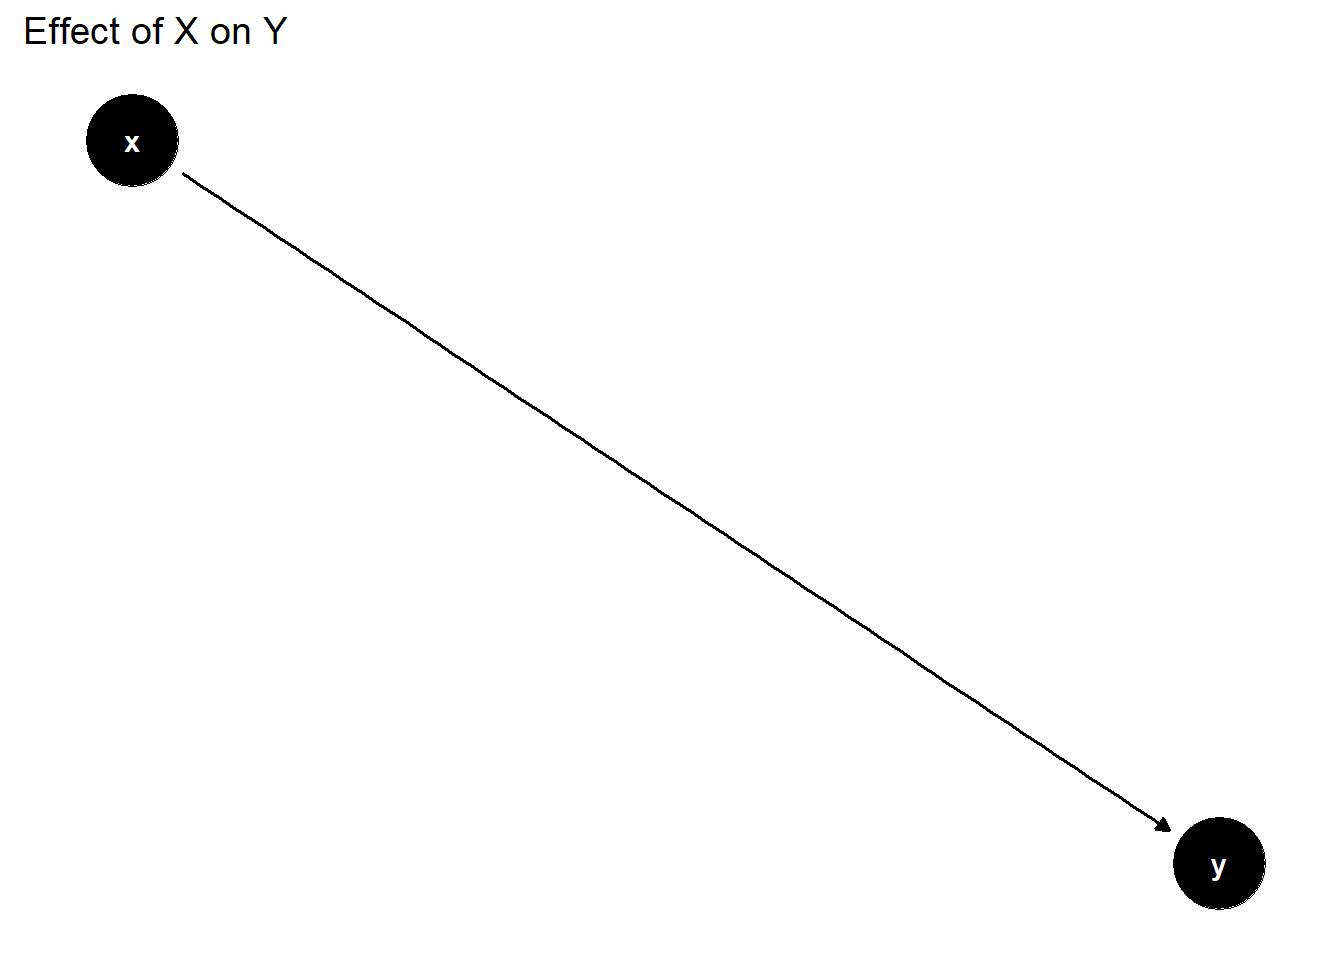
\includegraphics{DAG_files/figure-pdf/fig-dag-1.pdf}

}

\caption{\label{fig-dag}Effect of X on Y}

\end{figure}%

\chapter{Notation}\label{notation}

Unlike a normal graph DAGs go in one direction. What I mean is that we
do not get cycles or feedback loops between the different nodes. This is
a DAG:

Because DAGs are used in Graph Theory we will use the same notation and
names that they use. Each ``variable'' is a node in the graph and each
``arrow'' represents the direction of the causal relationship.In the
example above we see an arrow going from x to y a this represents a
one-way causal relationship. We can think of the graph above as x being
the interest rate and y being the cost of borrowing money.

\begin{Shaded}
\begin{Highlighting}[]
\FunctionTok{library}\NormalTok{(ggdag)}
\FunctionTok{library}\NormalTok{(dagitty)}

\CommentTok{\# Define the non{-}causal DAG}
\NormalTok{dag\_non\_causal }\OtherTok{\textless{}{-}} \FunctionTok{dagify}\NormalTok{(y }\SpecialCharTok{\textasciitilde{}}\ErrorTok{\textasciitilde{}}\NormalTok{ x)}

\CommentTok{\# Plot the non{-}causal DAG}
\FunctionTok{ggdag}\NormalTok{(dag\_non\_causal) }\SpecialCharTok{+} 
  \FunctionTok{theme\_dag}\NormalTok{() }\SpecialCharTok{+}
  \FunctionTok{ggtitle}\NormalTok{(}\StringTok{"Non{-}causal relationship between X and Y"}\NormalTok{)}
\end{Highlighting}
\end{Shaded}

\begin{figure}[H]

\centering{

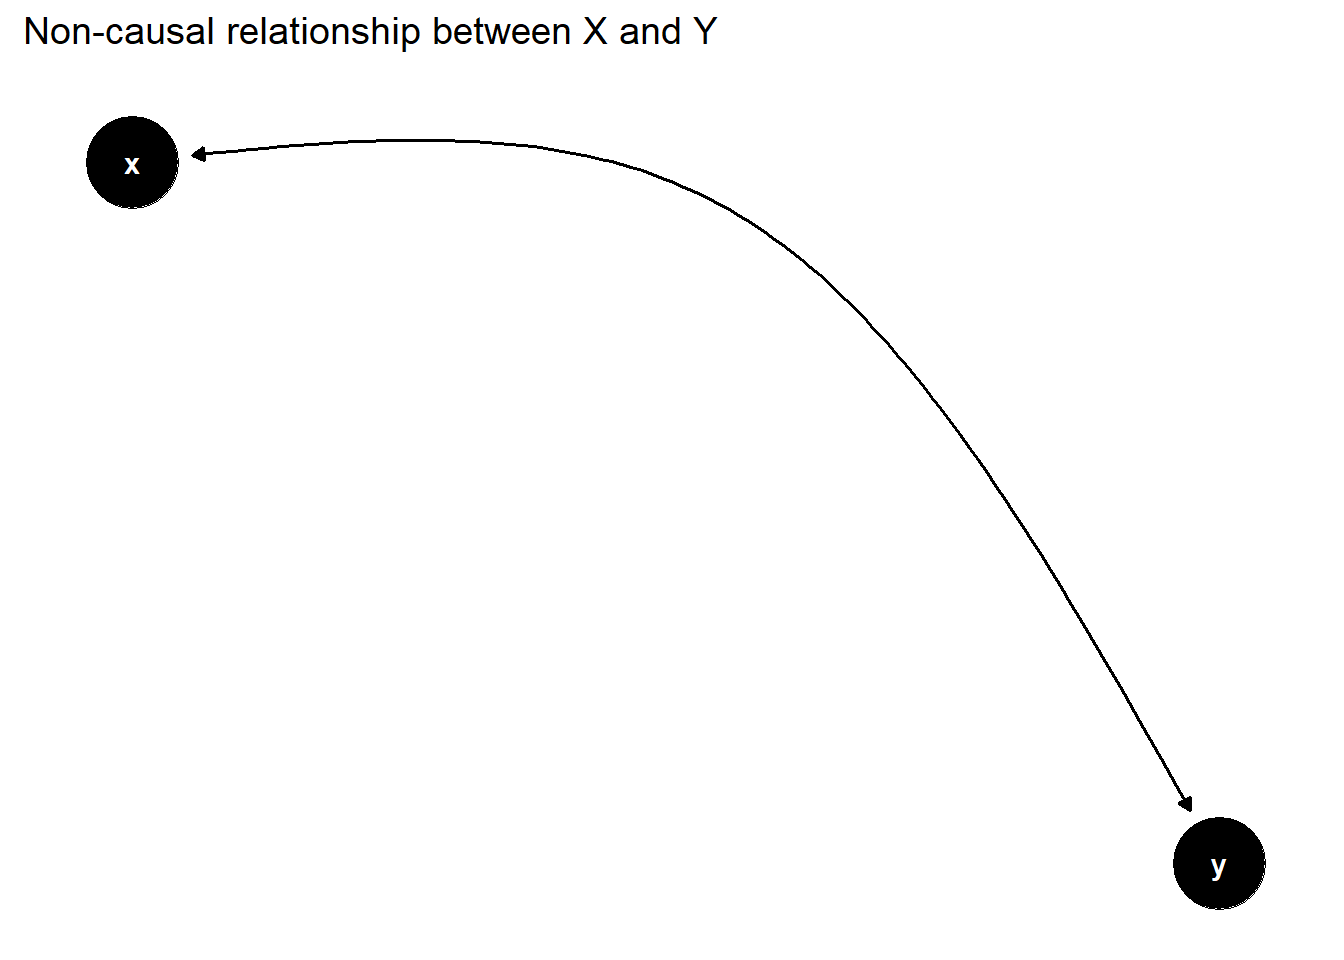
\includegraphics{DAG_files/figure-pdf/fig-non-causal-graph-1.pdf}

}

\caption{\label{fig-non-causal-graph}Non-causal relationship between X
and Y}

\end{figure}%

Here we can see a two way relationship which happens when x affects y
and y affects x. The ``arrows'' connecting the two nodes (variables) are
usually referred to as edges. When the edges are going in both
directions we usually called them bi-directed edges. However, it is
important to emphasize that this is not a DAG anymore but it represents
a feedback loop.

To drive this concept home we will look at a DAG and its corresponding
OLS regression equation. Please note that I am implicitly assuming that
I have identified the correct relationship between the variables which
is highly unlikely.

\begin{Shaded}
\begin{Highlighting}[]
\NormalTok{dag }\OtherTok{\textless{}{-}} \FunctionTok{dagify}\NormalTok{(}
\NormalTok{  Wages }\SpecialCharTok{\textasciitilde{}}\NormalTok{ Education,}
  \AttributeTok{labels =} \FunctionTok{c}\NormalTok{(}\StringTok{"Education"} \OtherTok{=} \StringTok{"Years of Schooling"}\NormalTok{, }\StringTok{"Wages"} \OtherTok{=} \StringTok{"Income"}\NormalTok{)}
\NormalTok{)}

\CommentTok{\# Plot the DAG}
\FunctionTok{ggdag}\NormalTok{(dag) }\SpecialCharTok{+} 
  \FunctionTok{theme\_dag}\NormalTok{() }\SpecialCharTok{+}
  \FunctionTok{ggtitle}\NormalTok{(}\StringTok{"DAG: Effect of Education on Wages"}\NormalTok{)}
\end{Highlighting}
\end{Shaded}

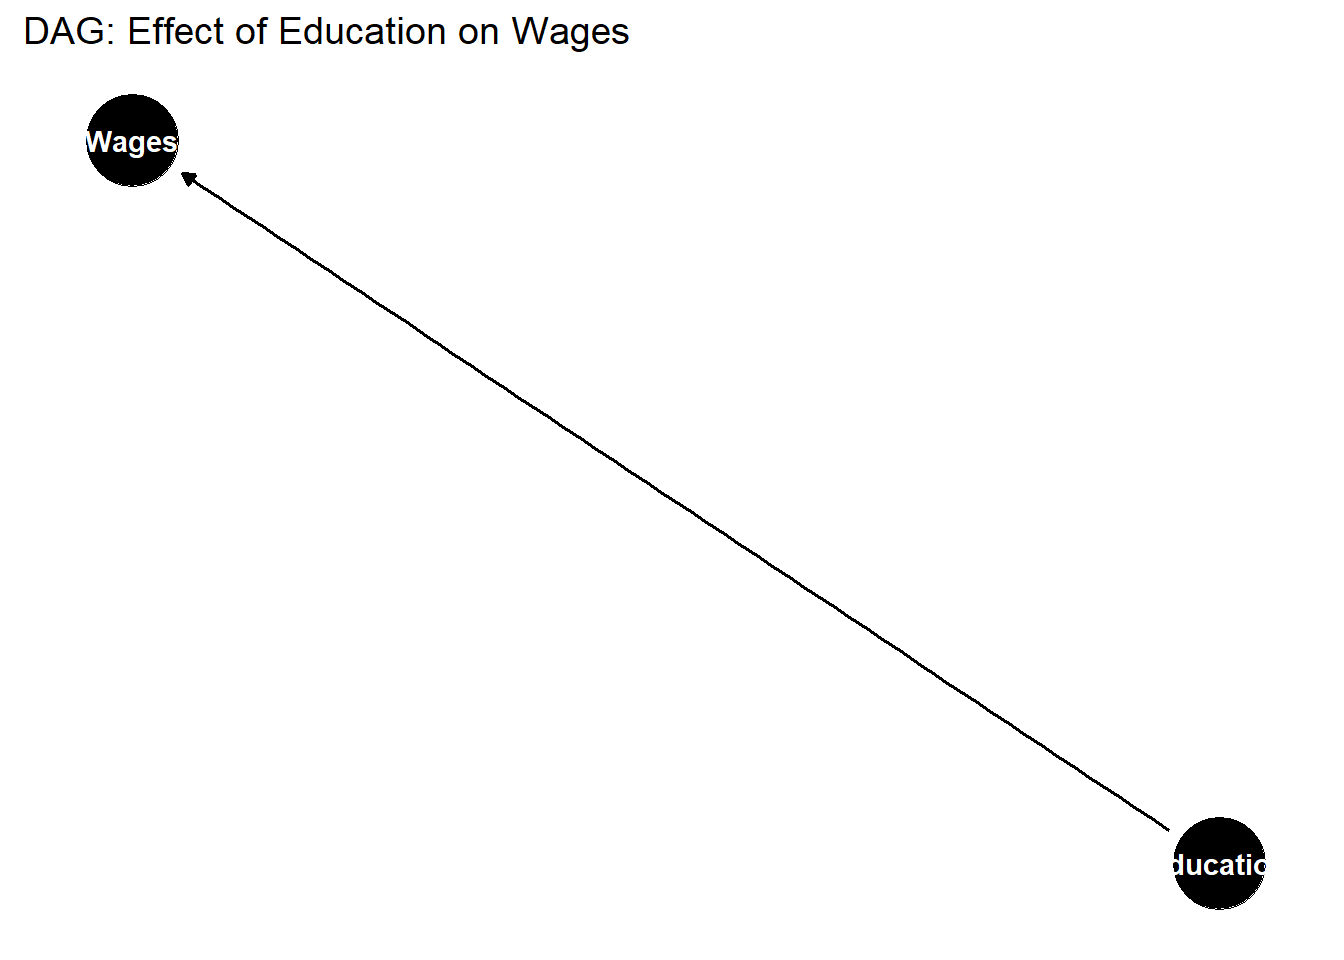
\includegraphics{DAG_files/figure-pdf/education-wage-dag-1.pdf}

This DAG represents the following OLS equation:

\[
\text{Wages} = \beta_0 + \beta_1 \text{Education} + \varepsilon
\]

Regardless of whether this is the true OLS regression from wages is
irrelevant. You'd be quick to notice that there is one thing
differentiating this OLS equation from the DAG. This key differentiating
aspect is the error term. In OLS regressions we usually assume that the
error term is white noise of mean zero. However, a DAG would take it a
step further an assume that this is the ultimate true relationship of
the data generating process and there is no room for error.

You might be asking yourself what is the point of all of this? Why are
we complicating the material with extra definitions and extra notation?

\chapter{Why are DAGs important for
Microeconometrics?}\label{why-are-dags-important-for-microeconometrics}

\section{Causality}\label{causality-1}

DAGs are useful when it comes to drawing causal relationships between
variables. If X causes Y but Y does not cause X then we can represent
this by the following graph:

\begin{Shaded}
\begin{Highlighting}[]
\NormalTok{dag1 }\OtherTok{\textless{}{-}} \FunctionTok{dagify}\NormalTok{(}
\NormalTok{  Y }\SpecialCharTok{\textasciitilde{}}\NormalTok{ X,}
  \AttributeTok{labels =} \FunctionTok{c}\NormalTok{(}\AttributeTok{X =} \StringTok{"X"}\NormalTok{, }\AttributeTok{Y =} \StringTok{"Y"}\NormalTok{)}
\NormalTok{)}

\FunctionTok{ggdag}\NormalTok{(dag1) }\SpecialCharTok{+}
  \FunctionTok{theme\_dag}\NormalTok{()}
\end{Highlighting}
\end{Shaded}

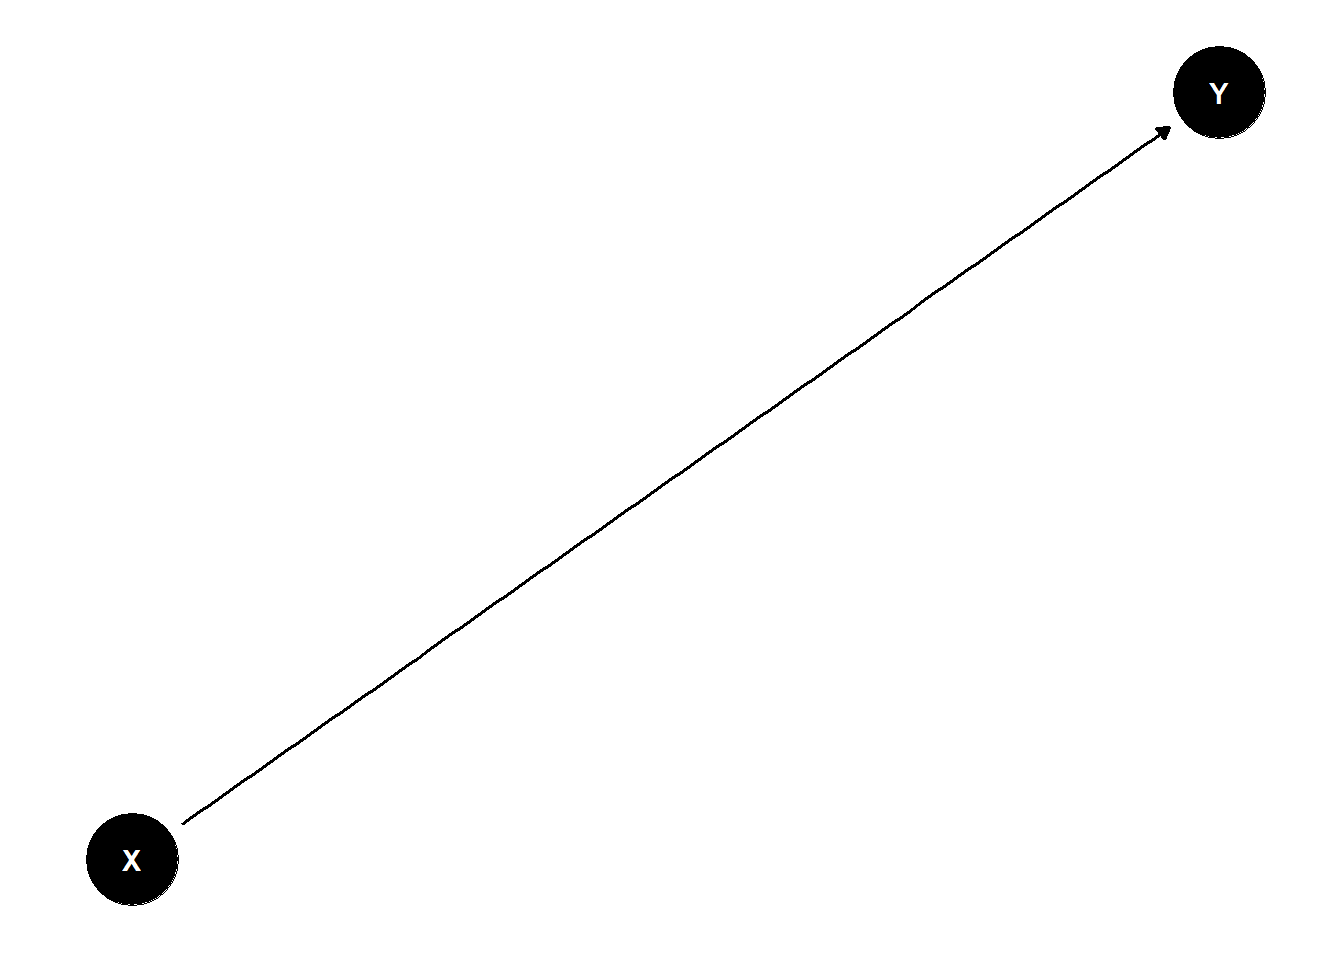
\includegraphics{DAG_files/figure-pdf/unnamed-chunk-4-1.pdf}

We can have a mediator between X and Y. So, X affects Y through Z.

\begin{Shaded}
\begin{Highlighting}[]
\NormalTok{dag2 }\OtherTok{\textless{}{-}} \FunctionTok{dagify}\NormalTok{(}
\NormalTok{  Y }\SpecialCharTok{\textasciitilde{}}\NormalTok{ Z,}
\NormalTok{  Z }\SpecialCharTok{\textasciitilde{}}\NormalTok{ X,}
  \AttributeTok{labels =} \FunctionTok{c}\NormalTok{(}\AttributeTok{X =} \StringTok{"X"}\NormalTok{, }\AttributeTok{Z =} \StringTok{"Mediator Z"}\NormalTok{, }\AttributeTok{Y =} \StringTok{"Y"}\NormalTok{)}
\NormalTok{)}

\FunctionTok{ggdag}\NormalTok{(dag2) }\SpecialCharTok{+} 
  \FunctionTok{theme\_dag}\NormalTok{() }\SpecialCharTok{+}
  \FunctionTok{ggtitle}\NormalTok{(}\StringTok{"DAG with Mediation: X affects Z, and Z affects Y"}\NormalTok{)}
\end{Highlighting}
\end{Shaded}

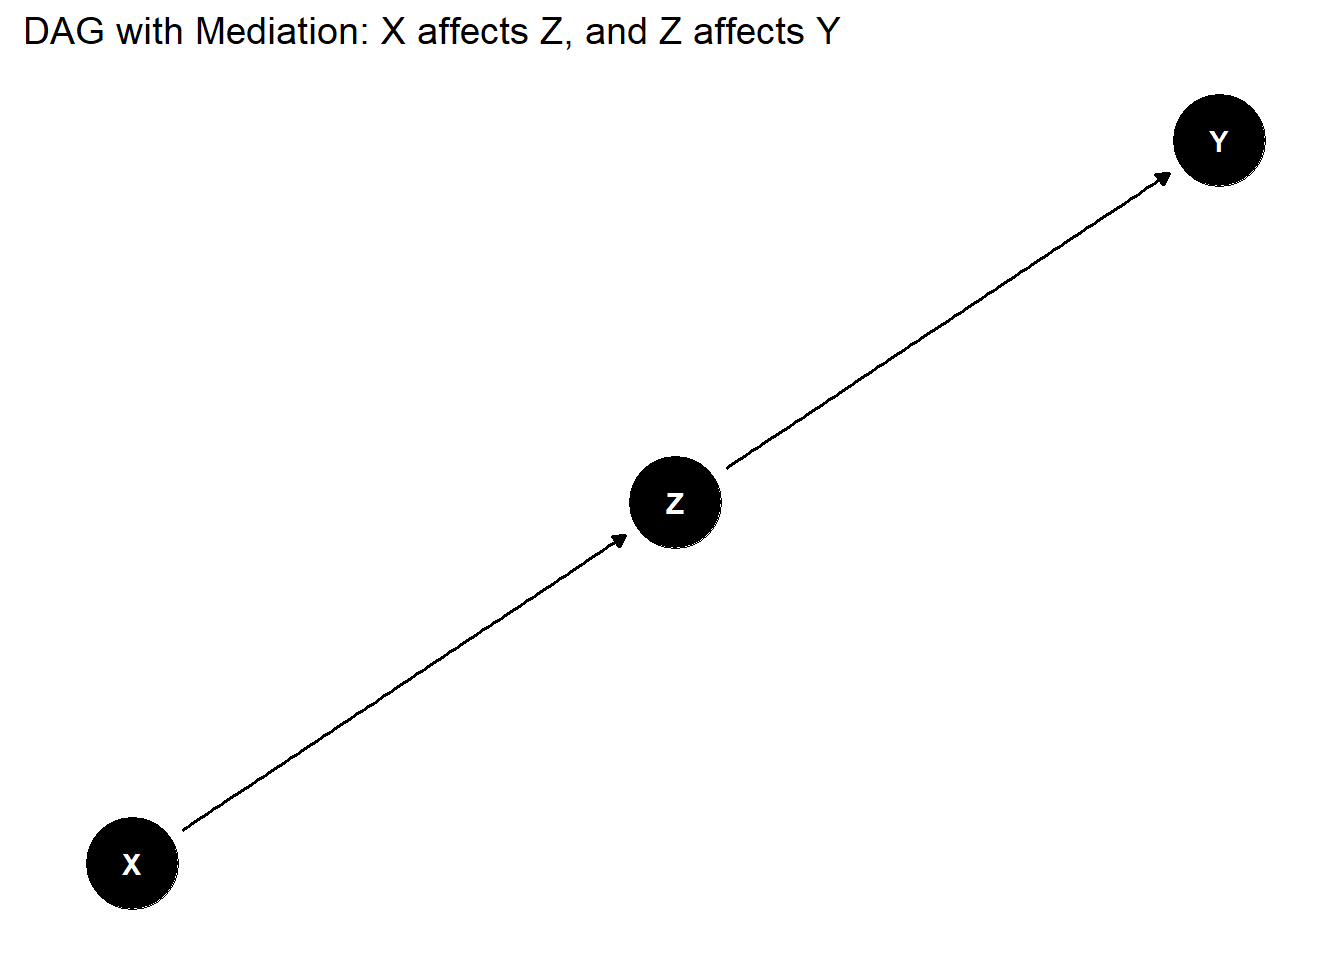
\includegraphics{DAG_files/figure-pdf/unnamed-chunk-5-1.pdf}

A real life example of this \(X\) being technological innovation, \(Z\)
being productivity and \(Y\) is Economic growth. Please note that this
is just an example and you could find evidence that does not support
this simplified version of reality.

DAGs could also help us to visualise some assumptions we as
econometricians make. We could represent confounders in DAGs.

\begin{description}
\item[Confounder]
In causal inference a confounder is a variable that influences both the
dependent variable and the independent variable causing a spurious
association
\end{description}

\begin{Shaded}
\begin{Highlighting}[]
\NormalTok{dag3 }\OtherTok{\textless{}{-}} \FunctionTok{dagify}\NormalTok{(}
\NormalTok{  Y }\SpecialCharTok{\textasciitilde{}}\NormalTok{ X }\SpecialCharTok{+}\NormalTok{ M,}
\NormalTok{  X }\SpecialCharTok{\textasciitilde{}}\NormalTok{ M,}
  \AttributeTok{labels =} \FunctionTok{c}\NormalTok{(}\AttributeTok{X =} \StringTok{"Education Intervention"}\NormalTok{, }\AttributeTok{Y =} \StringTok{"Job Performance"}\NormalTok{, }\AttributeTok{M =} \StringTok{"Motivation Level"}\NormalTok{),}
  \AttributeTok{exposure =} \StringTok{"X"}\NormalTok{,}
  \AttributeTok{outcome =} \StringTok{"Y"}
\NormalTok{)}

\FunctionTok{ggdag}\NormalTok{(dag3, }\AttributeTok{text =} \ConstantTok{TRUE}\NormalTok{) }\SpecialCharTok{+}  
  \FunctionTok{theme\_dag}\NormalTok{() }\SpecialCharTok{+}
  \FunctionTok{ggtitle}\NormalTok{(}\StringTok{"DAG: Education Intervention\textquotesingle{}s Effect on Job Performance with Motivation Level as a Confounder"}\NormalTok{)}
\end{Highlighting}
\end{Shaded}

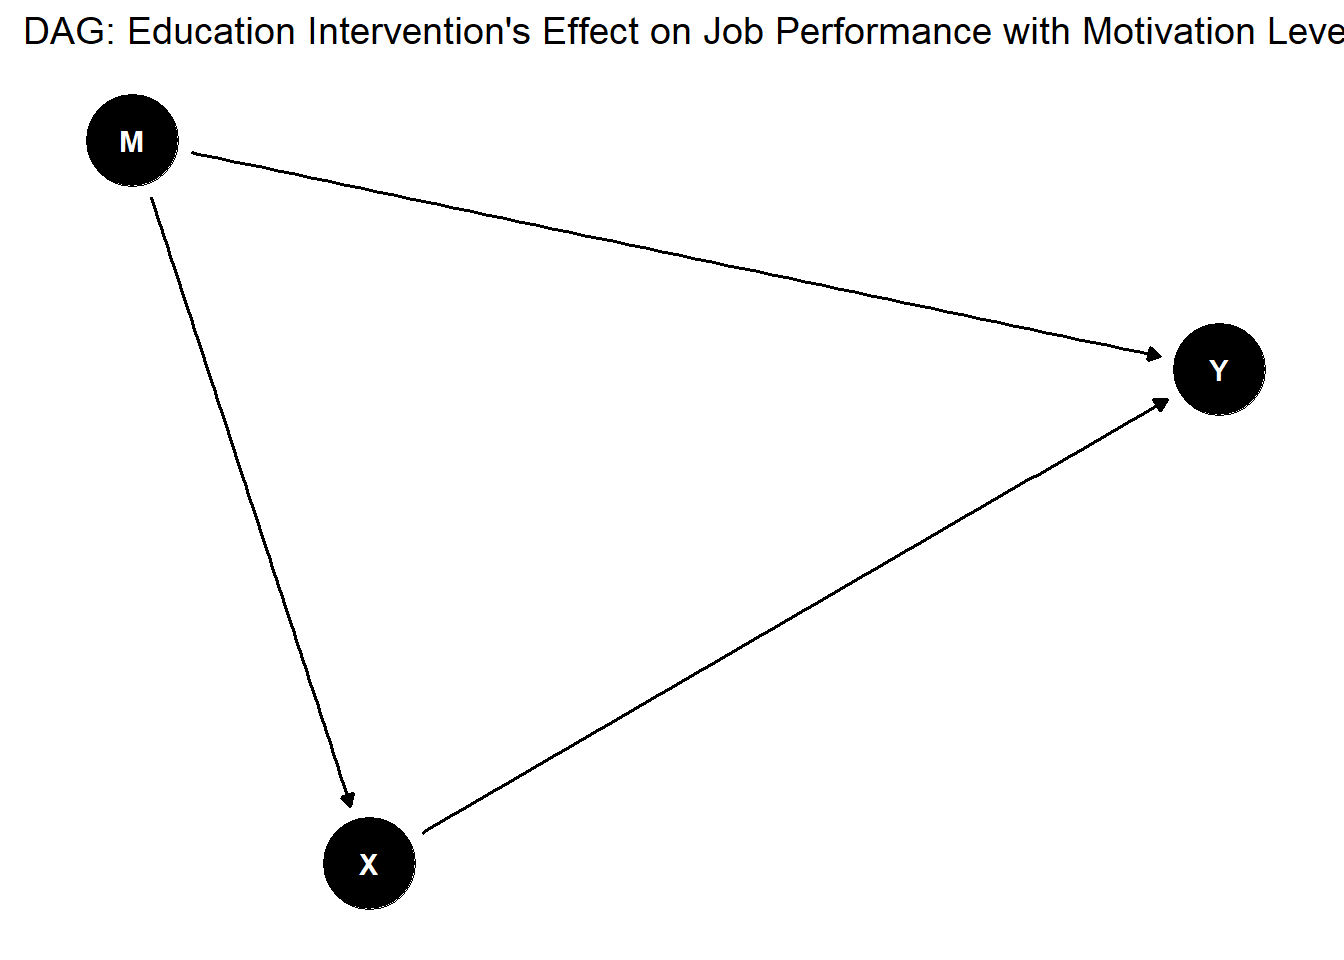
\includegraphics{DAG_files/figure-pdf/unnamed-chunk-6-1.pdf}

\begin{Shaded}
\begin{Highlighting}[]
\NormalTok{adjustedSet }\OtherTok{\textless{}{-}} \FunctionTok{adjustmentSets}\NormalTok{(dag3)}
\FunctionTok{print}\NormalTok{(adjustedSet)}
\end{Highlighting}
\end{Shaded}

\begin{verbatim}
{ M }
\end{verbatim}

\chapter{Visualising Assumptions:}\label{visualising-assumptions}

\begin{description}
\item[Exogeneity Assumption]
In simple terms, the exogeneity assumption that all the explanatory
variables are exogenous and therefore not influenced by other variables
in the model or by the dependent variable.
\end{description}

This can be illustrated quite nicely using DAGs. Imagine you are
investigating the effect of an educational program \(X\) on job
performance \(Y\), with motivation \(M\) as a mediator then if the
exogeneity assumption hold you would get something like this:

\[
X \rightarrow M \rightarrow Y
\]

\chapter{Visualising Instrumental
Variables}\label{visualising-instrumental-variables}

Instrumental variables (IV) like the name suggest are variables which
are used as instruments to control for confounding and measurement error
in observational studies.
\href{https://en.wikipedia.org/wiki/John_Snow}{John Snow}, one of the
fathers of modern epidemiology is widely recognised from his work during
the cholera outbreak in the mid-19th century. You might ask yourself,
what does epidemiology and cholera have to do with IVs? well\ldots{}
bare with me for a second.

In 19th century London cholera was a big thing and it was taking
hundreds of thousands of lives a year. People at that time thought that
cholera was caused by ``bad air'' so they basically thought that cholera
was transmitted via the air. Snow had a theory and to prove it he used
instrumental variables before the term or the formality of instrumental
variables was discovered.

To test his hypothesis that cholera was transmitted through the water
rather than through air he used the proximity to the Broad Street pump
in London as an instrument. Individuals near the pump are more likely to
use it but are not inherently more likely to contract cholera from other
reasons. For now, we will call this IV \(Z\). The treatment is drinking
water from the Broad Street Pump \(W\). The outcome variable is the
cholera infection which we will denote \(C\) and we let \(U\) denote the
unobserved confounders which could be factors such as individual health
(not great at the time) , sanitation practices, or other ways of
contracting cholera not from the pomp.

As you can already be thinking using the proximity as the IV helps
isolate the effect of the contaminated water on cholera.

\begin{Shaded}
\begin{Highlighting}[]
\NormalTok{IV}\OtherTok{\textless{}{-}}\FunctionTok{dagify}\NormalTok{(C}\SpecialCharTok{\textasciitilde{}}\NormalTok{W}\SpecialCharTok{+}\NormalTok{U,W}\SpecialCharTok{\textasciitilde{}}\NormalTok{U, W}\SpecialCharTok{\textasciitilde{}}\NormalTok{Z) }
\NormalTok{coords}\OtherTok{\textless{}{-}}\FunctionTok{list}\NormalTok{(}\AttributeTok{x=}\FunctionTok{c}\NormalTok{(}\AttributeTok{W =} \DecValTok{0}\NormalTok{, }\AttributeTok{U =} \DecValTok{1}\NormalTok{, }\AttributeTok{C =} \DecValTok{2}\NormalTok{, }\AttributeTok{Z=}\SpecialCharTok{{-}}\DecValTok{1}\NormalTok{),}
          \AttributeTok{y=}\FunctionTok{c}\NormalTok{(}\AttributeTok{W =} \DecValTok{0}\NormalTok{, }\AttributeTok{U =} \FloatTok{0.1}\NormalTok{, }\AttributeTok{C =} \DecValTok{0}\NormalTok{, }\AttributeTok{Z=}\DecValTok{0}\NormalTok{)) }
\NormalTok{coords\_df}\OtherTok{\textless{}{-}}\FunctionTok{coords2df}\NormalTok{(coords)}
\FunctionTok{coordinates}\NormalTok{(IV)}\OtherTok{\textless{}{-}}\FunctionTok{coords2list}\NormalTok{(coords\_df)}
\FunctionTok{ggdag}\NormalTok{(IV)}\SpecialCharTok{+}\FunctionTok{theme\_dag\_blank}\NormalTok{()}
\end{Highlighting}
\end{Shaded}

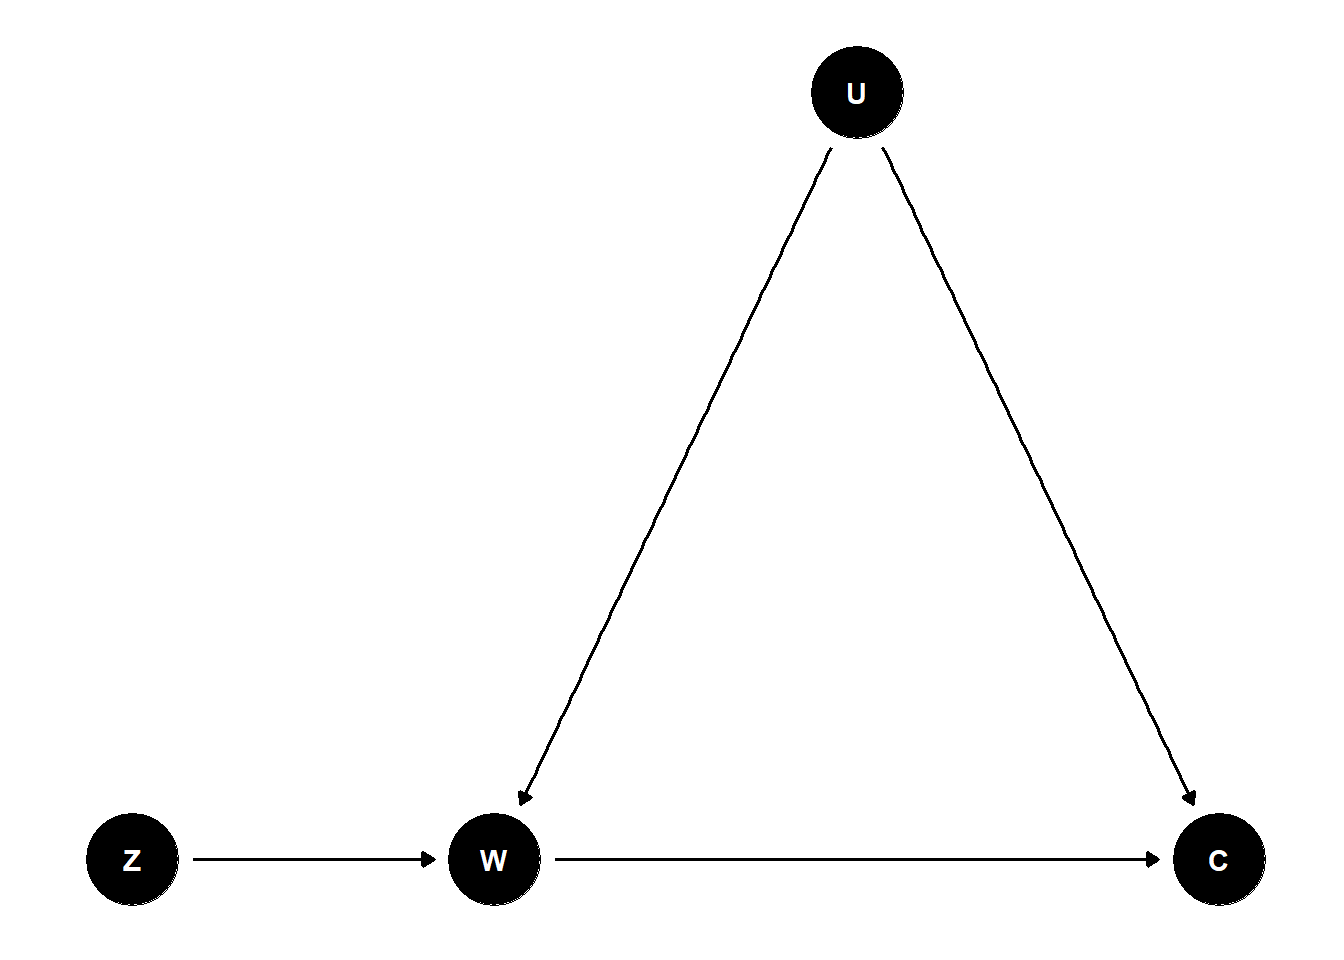
\includegraphics{DAG_files/figure-pdf/unnamed-chunk-7-1.pdf}

\begin{Shaded}
\begin{Highlighting}[]
\CommentTok{\# Code borrowed from https://donskerclass.github.io/EconometricsII/ControlandIV.html}
\end{Highlighting}
\end{Shaded}

It is important to notice that the instrument \(Z\) (proximity to the
pump) for cholera infection \(C\) satisfies both the relevance
assumption and the exogeneity assumption which makes this a valid IV.



\end{document}
